\documentclass[a4paper,12pt,twoside]{book}
\usepackage[utf8]{inputenc}
\usepackage[english]{babel}
%\usepackage{fontspec}
%\setmainfont[
%  Ligatures=TeX,
%  Extension=.otf,
%  BoldFont=cmunbx,
%  ItalicFont=cmunti,
%  BoldItalicFont=cmunbi,
%  SlantedFont=cmunsl
%]{cmunrm}

%\usepackage{polyglossia}
%\setmainlanguage{spanish}

\usepackage[c5paper]{geometry}
%\geometry{inner=2.5cm,outer=2.5cm,bmargin=3.2cm}
%\usepackage[DIV=14,BCOR=2mm,headinclude=true,footinclude=false]{typearea}

%\usepackage{ulem} %Hace que \emph sea subrayar

%\usepackage[p,osf]{scholax}
%% T1 and textcomp are loaded by package. Change that here, if you want
%% load sans and typewriter packages here, if needed

\usepackage{ebgaramond}
%\usepackage[type1]{libertine} % Linux Libertine for zweispaltige Texte
%\usepackage{textcomp}% Required to get special symbols
\usepackage[scaled=.8]{DejaVuSansMono}% FiraMono Typewriter font
\usepackage{PTSansNarrow} 
%\gilliuscondensed
%\usepackage[sfdefault]{FiraSans}
%\usepackage{bm}% Extra bold faces
%\usepackage[lf]{carlito}

\usepackage{lettrine} %Capital letters at the beginning of a chapter
\usepackage[activate={true,nocompatibility},final,tracking=true,kerning=true,spacing=true,factor=1100,stretch=10,shrink=10]{microtype}
\SetTracking{encoding={*}, shape=sc}{-20} % versalitas menos separadas
% activate={true,nocompatibility} - activate protrusion and expansion
% final - enable microtype; use "draft" to disable
% tracking=true, kerning=true, spacing=true - activate these techniques
% factor=1100 - add 10% to the protrusion amount (default is 1000)
% stretch=10, shrink=10 - reduce stretchability/shrinkability (default is 20/20)

%\usepackage{array,multirow,booktabs,colortbl,chngcntr} % El último es para counterwithout;
\usepackage[strict]{changepage}
%\usepackage{caption}
%\captionsetup{format=plain,labelsep=newline,labelfont={small,sc},
%textfont={small,it},singlelinecheck=false}
\usepackage[Bjornstrup]{fncychap} % Para cabeceras de capítulos sofisticados:     Sonny,    Lenny,    Glenn,    Conny,    Rejne,    and Bjarne.

\usepackage{graphicx,wrapfig,booktabs,multicol,tabularx} % wallpaper: poner imágenes de fondo; wrapfigure: figuras a un lado del texto
%\graphicspath{{figures/}}
\usepackage{fancyhdr}
\usepackage{emptypage,pdfpages,fancybox} % Para que las páginas en blanco no tengan encabezado;
\usepackage{enumitem} %paralist: para compactenum, enumerate sin espacios
%\setlist[itemize]{nosep} %Espacio entre items en itemize
\usepackage[hyperref]{xcolor}
\usepackage[hidelinks]{hyperref}
\usepackage{xurl}

%\usepackage{minipage}

%\usepackage{quotchap} %Encabezados de capítulos
\usepackage{syntonly,verbatim}
%\syntaxonly

\usepackage{setspace,xspace} % xspace: Da \xspace para no tener que poner {} después de los comandos; pdflscape: páginas en horizontal;

\newenvironment{quotex}{\begin{quote}\small}{\end{quote}}
\newenvironment{quotationx}{\begin{quotation}\small}{\end{quotation}}


\begin{document}

% Por alguna razón, los marginados se creaban al revés. Así los corrijo. Feo, pero eficaz:
\let\tmp\oddsidemargin
\let\oddsidemargin\evensidemargin
\let\evensidemargin\tmp
\reversemarginpar

%\setcounter{secnumdepth}{4} % Para que llegue a numerar hasta las subsubsecciones;
%\renewcommand{\heavyrulewidth}{0.14em} % Grosor de las líneas extremas de las tablas;
%\renewcommand\thempfootnote{\alpha{mpfootnote}} % Símbolo de notas dentro de minipage
%\let\oldcaptionof\captionof
%\renewcommand{\captionof}[2]{\oldcaptionof{#1}{\newline \textit{#2} }}
%\renewcommand{\tablename}{Tabla}
%\counterwithout{figure}{chapter}
%\counterwithout{table}{chapter} % Así la numeración es 1, 2, 3... y no 1.1, 1.2... y no reinicia la num. en cada capítulo;

%\providecommand{\ggl}{\guillemotleft}
%\providecommand{\ggr}{\guillemotright\xspace}
\providecommand{\flright}[1]{\begin{flushright}#1\end{flushright}}
\providecommand{\flrightit}[1]{\begin{flushright}\itshape #1\end{flushright}}
%\renewcommand\UrlFont\sffamily
\urlstyle{tt}

\pagestyle{fancy}
\renewcommand{\sectionmark}[1]{\markright{#1}}
\renewcommand{\chaptermark}[1]{\markboth{#1}{}}

%Portada:
%\includepdf{00Portada}

\frontmatter
%
%\onehalfspacing
%\pagenumbering{Roman} %gobble es como empty

%\include{preindice}

%\fancyhf{}
%\fancyhead[LE]{\small \textbf{\thepage}$\quad$ Índice general}
%\fancyhead[RO]{\small Índice general $\quad$\textbf{\thepage}}
%\clearpage
\tableofcontents

%\doublespacing
\mainmatter

\fancyhf{}
\fancyhead[LE]{\small \thepage$\quad${\scshape\chaptername{} \thechapter}: \nouppercase{\itshape\leftmark}}
\fancyhead[RO]{\small \textsc{Section }\thesection{}: \nouppercase{\itshape\rightmark} $\quad$\upshape\thepage}
%\cfoot{\bfseries\thepage}

\pagenumbering{arabic}

%\onehalfspacing

% introductorios

\chapter{Introduction}
\section{The Gift of 1000 Sages}

We, as a human race, have been blessed with a great number of Prophets, starting with Adam, Seers, Sages, Saints, Philosophers, Doctors, Poets, Worthies, and other Great Men. Most have been forgotten or known by name only. The reason to prefer the antique thinkers is because they have stood the test of time. Centuries of scholars have analyzed and commented on their works, so those who “survive” are worth our time.

\begin{wrapfigure}{ht}{.35\textwidth}
 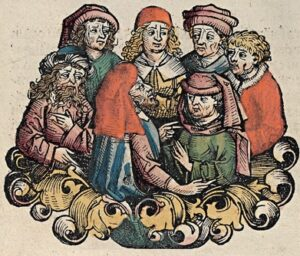
\includegraphics[scale=.5]{a20210908TheGiftof1000Sages-img001.jpg} 
\end{wrapfigure}

There may be contemporaries at their level, but that may be difficult to discern. They can be treated with caution, more especially if they claim any sort of novelty. Those who can make clear the ideas of the ancients are better guides.

I was struck at one time by Vladimir Solovyov's nonchalant comment that Christianity did not create a new metaphysic, but was instead based on historical events. That made sense of Rene Guenon's famous claim of a common metaphysics that underlie the major religious traditions. There will be incompatibilities in their exoteric teachings which are based on historical events but the metaphysical assumptions should align.

Although Guenon make progress in this area, there is still much to be said about the common metaphysics. Given the two texts I am working with: \textbf{Jacques Maritain}'s \emph{Introduction to Philosophy} and \textbf{Syed Naquid}'s \emph{Prolegomena to Islamic Metaphysics}, this thought jumped right up into consciousness:

\begin{quotex}
If I remove the Latin from Maritain's book and the Arabic from Naquid's book, the metaphysical principles are virtually indistinguishable. I could go on and on, which I shall do over time, but I'll start with this one example: both agree that regarding God, essence and existence are the same. All else follows.

\end{quotex}
This reminded me of what \textbf{C S Lewis} wrote in \emph{The Discarded Image}: There are ancient texts which are not obviously Christian or Pagan, given that their worldviews were so closely aligned with each other. In the same vein, the ideas that Lewis assumed were Christian turn out also to be Islamic. Essence, existence, substance, act, potentiality and so on have the same meanings. These will be explored in details, not as arguments but as expository.

Since the West has effectively abandoned metaphysics, it needs to be reinvigorated by a tradition that still accepts it. Here are some principles to ponder.

\paragraph{Three Worlds}
There are three worlds: the Corporeal, the Imaginal, the Spiritual, corresponding to body, soul, and spirit. They are not independent, so by the Law of Correspondence, what happens in the celestial realm is reflected in the imaginal realm, and ultimately in the corporeal world.

Therefore the world has an inside as well as an inside. Knowledge begins in the senses and we can advance to the spiritual through a process of abstraction. Things and events have a representation and meaning in the life of the soul. To reach the essence of the thing, it is necessary to abstract even from that image into pure thought.

It is one thing to understand the essence of a species like a lion, for example. It is more difficult to understand the essence of an individual, such as someone you may know and love. Religious dogmas, then, are even more difficult. If you try to visualize it, you will be mistaken. You can recite the Apostle's Creed daily, until it loses its meaning. If you are visualizing beings in Heaven as if you are some objective onlooker, you will miss the point. It is also immoral since it is an idol.

This project is an attempt to recall the collective wisdom of humankind, not as a new theory, but as an old truth.


\flrightit{Posted on 2021-09-08 by Cologero}

\begin{center}* * *\end{center}

\begin{footnotesize}\begin{sffamily}

\texttt{Tom on 2021-09-10 at 09:31 said: }

” If you are visualizing beings in Heaven as if you are some objective onlooker, you will miss the point. It is also immoral since it is an idol “.

Just wondered how to square that statement with Tomberg's statement that ” “There is not a shadow of doubt for anyone who takes the spiritual life of mankind seriously, even if he is short of authentic spiritual experience, that the Blessed Virgin is not an ideal only, nor a mental image only, nor an archetype of the unconscious (of depth-psychology), nor, lastly, an occultistic egregore, but rather a concrete and living individuality – like you or I – who loves, suffers, and rejoices. “?\newline
Tomberg's quote is from this site :

\url{https://corjesusacratissimum.org/2012/07/on-degeneration-disaster-and-war-valentin-tomberg-and-the-lady-of-all-nations/}

In general I think the question is how to reconcile ” metaphysical ” formlessness as ontologically superior to form with the statements like this or the fact that Jesus is described in the Gospels as “sitting at the right hand of the Father “. Or that personality is higher than individuality. In other word aren't there bodies in heaven “” Even Dante suggests as much .


\hfill

\texttt{Cologero on 2021-09-10 at 10:09 said: }

There is nothing to reconcile. E.g., she is not a “mental image”. I would change “individuality” to “personality”, but she is as real as “you or I”. It is necessary to understood what it means to be a person, an “I”.

The explanation of the “Person” is on the schedule for a near future post, but it needs a build up. I think it will clarify a lot.


\hfill

\texttt{Cologero on 2021-09-10 at 11:44 said: }

Let me add come further clarifications, although these topics have appeared over and over again as posts.

The soul after death does not exist solely in the Intellectual or Celestial Realm, but also in the Imaginal Realm. So there will be appearances of bodies, but glorified spiritual bodies with the properties of impassibility, agility, clarity, and subtlety.

The physical realm is pure potentiality and thus part of Non-Being, so it is an error to assume that every experience is somehow physical.

Also, with metaphysical realization, i.e. awareness of being a Person, the Person exists in all his states of being simultaneously. Of course, the extent of this depends on the ability and nobility of the person.


\hfill

\texttt{Tom on 2021-09-10 at 12:17 said: }

Thank you for the extra clarification.


\hfill

\end{sffamily}\end{footnotesize}

%Sugiere un índice: Tomismo, no-ser+infinito+no-dualidad vedantotaoista, naturaleza tripartita del hombre, todo esto en la tradición hermética, y todo esto en práctica espiritual
\section{Guenon, Maritain, Thomism}

\emph{Prolegomena to any future Western metaphysics.}

\paragraph{Meeting of the Minds}
In 1921, the great Thomist philosopher Jacques Maritain criticized Rene Guenon for participating in the rebirth of gnosis, the “mother of heresies”. Guenon responded, “It would make as much sense to speak of Catholicism as the father of Protestantism. In fact, you are simply confusing gnosis with Gnosticism.”

“If you take the word `gnosis' in its true sense, that of pure knowledge, as I always do when I happen to use it … Gnosis so understood — and I refuse to understand it otherwise — cannot be called the mother of heresies. That would be the same as saying that the truth is the mother of errors.”

To be clear, by `gnosis' or `wisdom' as Evola usually called it, Guenon is referring to a state of being, not to a science or a set of doctrines to learn. At that point in his career, Guenon was involved in studying eastern doctrines on the one hand, and Christian symbolism on the other.

On May 25, 1925, Guenon participated in a round table discussion that included Maritain, where Guenon defended Hindu metaphysics. Guenon denied that it was either pantheist or idealist, contrary to academic consensus. Rather, it is connected more closely to the Aristotelian tradition, including the scholastic philosophy of the Middle Ages as exemplified by Thomas Aquinas.

Maritain objected because, from his point of view, this alliance between eastern and Catholic metaphysics is “an inadmissible subordination and the ruin of the distinction between the natural and supernatural order, between nature and grace.” For Maritain, metaphysics is not beyond theology, the “supreme science”. Although Maritain had an authentic intellectual respect for Guenon, he eventually forced Guenon out of contributing to Catholic journals, and an opportunity was lost to further develop Thomism more fully and completely.

\paragraph{Maritain's Misunderstanding}
First of all Maritain fails to grasp Guenon's distinction between philosophy and metaphysics, so he thinks from the perspective of the former. Since metaphysics is by definition the study of supernature (“beyond physics”), the distinction between the natural and the supernatural order is preserved. Maritain simply asserts that the supernatural order can be grasped only by faith and not by any sort of gnosis; this is remarkable, since as Guenon reminds us, for “Aristotle and his Scholastic successors … the intellect was in fact that faculty which possessed a direct knowledge of principles.” In other words, Thomism does indeed admit a gnosis, though its full consequences have not been incorporated into theological thinking insofar as it may present a threat to the primacy of faith.

\paragraph{Further background}
Evola also accepts Guenon's judgment about Thomism, which he sees as part of the process of “rectification”. Interestingly enough, John Woodroffe, although he does not explicitly refer to the Aristotelian tradition (as far as I can recall), similarly denies that Tantrism is “idealist”, but is likewise “realist”. In his \emph{Introduction to the Study of Hindu Doctrines}, Guenon develops this topic more fully. Although at one point he claims that the only Western metaphysics is that of Aristotle and the Scholastics, he clarifies: 

\begin{quotex}
We do not include the Alexandrians, however, upon whom Oriental influences came to be exercised in a direct manner. 

\end{quotex}
The Alexandrians would include St Anthony the Great\footnote{\url{https://www.gornahoor.net/?p=1224}} and what we call the Hermetists\footnote{\url{https://www.gornahoor.net/?p=1256}}.

\paragraph{Future Directions}
Where Thomism falls short is that it is a metaphysic of Being. It needs to be enhanced with an understanding of non-being as described in the \textbf{Multiple States of Being}. Catholic theology is hampered somewhat by the Eighth Ecumenical Council which denied the tripartite nature of man as spirit, soul, and body. (The Eastern churches don't accept this council.) This needs to be overcome, so elements from the \textbf{Great Triad} and \textbf{Man and his Becoming according to the Vendanta} can be incorporated.

In summary: to recreate a Western metaphysic for our time one would:

\begin{enumerate}
\item Begin with Thomism 
\item Incorporate an understanding of non-being, infinity, and non-duality from the Vedanta and Taoism 
\item Develop more fully the understanding of tripartite nature of man 
\item Integrate it with the ancient Hermetic tradition 
\item Integrate this with a spiritual practice so it arises from a true gnosis and does not devolve into yet another intellectualizing philosophy or theology 
\end{enumerate}
The young man who will take up this task may already have been born.


\hfill

Reference: \emph{Rene Guenon: Le philosophe invisible} by Jean-Luc Maxence. All translations from the French are mine.

\flrightit{Posted on 2010-12-15 by Cologero}

\begin{center}* * *\end{center}

\begin{footnotesize}\begin{sffamily}
\texttt{James O'Meara on 2010-12-15 at 23:27 said: }

Oddly enough, that 5 step program reminds me of Alan Watts' intellectual journey [see his Beyond Theology or In My Own Way] although he may have gone a bit astray on the last step…


\hfill

\texttt{Cologero on 2010-12-16 at 00:31 said: }

Perhaps I was just recalling ideas hidden in the unconscious from when I read those books many years ago.

I know someone who, as a young man, managed to get to San Francisco from Chicago in order to meet Mr. Watts. On his arrival, he looked up Watts in the phone book and called. His wife answered. There were noisy children in the background and the wife made some disparaging remarks about why Watts wasn't home … in particular referring to his drinking. Disillusioned, the young man left San Francisco, not having met Watts.


\hfill

\texttt{GF on 2010-12-17 at 12:11 said: }

Why not begin with Dionysius the Areopagite? He already has fully developed arguments on Non-Being and gnosis, and at least an implied understanding of tripartite nature. Do you include him among the Alexandrians? 

Which makes me think: If the finished doctrine is supposed to combine (Alexandrian) Hermetism with Thomism, as an admittedly superior leaven, isn't it truer to say that one should begin with the Alexandrians? As in fact Gornahoor has been doing?

But I see you say “for our time”: and I understand why *appearing* to begin with the Alexandrians would be impolitic in our time, at least among Catholics.


\hfill

\texttt{James O'Meara on 2010-12-17 at 12:14 said: }

How Watts went astray: searching and `finding' analogies btw esotericism and what would become the New Age, he confused the Taoist Sage with the stoned hippie or hot-tub psychologist:

“…SERIOUS PLAY [a very Wattsian idea] contains at the same time a serious warning: there is Play and play, there is the Magician and the magician; this is why anyone who confuses lack of concentration with concentration without effort…will necessarily become a CHARLATAN.” — Meditations on the Tarot


\hfill

\texttt{GF on 2010-12-17 at 12:17 said: }

Dionysius also has a conception of esoterism. So my `counter-proposal' is this:

\begin{enumerate}
\item Begin with Dionysius

\item Integrate with Thomism

\item Integrate with spiritual practise
\end{enumerate}

Your steps 2 and 3 are basically eliminated, and the represented order is more accurate (Thomism, being lesser, comes later).


\hfill

\texttt{James O'Meara on 2010-12-17 at 12:29 said: }

Again, oddly like Watts, who indeed began with Dionysius, published a translation of the Theologica Mystica whilst in the seminary in 1944 [!] and later republished it in his full hippie period, saying something like “Here had been the opportunity for Western theologians to close up shop and become schools of contemplation of the nameless, but instead they just kept chattering.” From 1 to 3, skipping 2?


\hfill

\texttt{GF on 2010-12-17 at 13:04 said: }

Yes, I suppose it comes down to that. St. Bernard himself, whose praises Guenon sung, had only contempt for the verbiage of philosophers and theologians. Though if a theological `ornamention' must be added, St. Thomas would be valuable.


\hfill

\texttt{Cologero on 2010-12-17 at 14:11 said: }

I might never have heard of Guenon were it not for Watts. He follows a familiar path … try to reform one's own “tradition”, get frustrated and turn East. And then fall into the confusion that Tomberg describes.


\hfill

\texttt{GF on 2010-12-17 at 14:12 said: }

One of the very interesting things about Dionysius is that he claims his written work is informed only by the `Oracles’ (Old and New Testaments) – and yet how different it is than sola scriptura Protestantism. So much depends on the atmosphere in which one lives. – In case you didn't know, James, Dionysius was Bishop of *Athens*.


\hfill

\texttt{Cologero on 2010-12-17 at 14:22 said: }

Yes, Dionysus, whom Aquinas quotes some 1200 times, is among the Alexandrians. I would regard the Aristotelean and Platonic perspectives as two \emph{darshanas}, or perspectives. We are well past the time for worrying about being “impolitic” about issues related to these topics since the era of persecution, at least in this area, is over. There is no need to convince anyone. This writer was driven from a self-described traditional Catholic forum for promoting Dionysius, so I wouldn't waste time in a futile debate.

What is required is a group effort to define and implement the task.


\hfill

\texttt{Cologero on 2010-12-17 at 14:38 said: }

In his commentary on Vatican II — an event which was pretty much pointless — Evola proposes his own program to reform the Catholic religion. I'll have to make time to translate it soon. Suffice it to say that I read Tomberg in that light, in particular the way he understands Bible stories. Evola concedes that St Clement of Alexandria's distinction between the gnostics (knowers) and believers was behind his own conception of “those who know and those who believe”.

Guido de Giorgio is a figure, close to both Guenon and Evola, who unfortunately remains unknown. While Guenon was turning East and Evola remained staunchly in the West, di Giorgio developed a synthesis of both. Like Gornahoor, he sees a continuity, not a break, from the ancient world through the Medieval period.


\hfill

\texttt{GF on 2010-12-17 at 15:25 said: }

“What is required is a group effort to define and implement the task.”

This is exactly why I ask you about Catholicism. If I'm reading you right, the outline of your plan would be the development of an order, which, like the Fransiscans and the Jesuits Tomberg cites, would replenish the Church from the outside. I gather that ultimately you are indifferent to the Church: if it can be bent to Traditional ends, use it; if not, forget it. So much for the Church: what of Christ Himself? 

I'm looking forward to the new translations.


\hfill

\texttt{Cologero on 2010-12-24 at 16:04 said: }

For those interested in the current state of Hinduism in India, this article may be of some interest: Rush Hour for the Gods.

\begin{quotex}
While the West often likes to imagine the religions of the East as deep wells of ancient, unchanging wisdom, in reality, much of India's religious identity is closely tied to specific social groups, caste practices and father-to-son lineages, all of which are coming under threat as Indian society transforms beyond recognition.

\end{quotex}

\hfill

\texttt{Cologero on 2010-12-24 at 16:19 said: }

Some points:

\begin{itemize}
\item Thomism takes non-being into account in the distinction between \textbf{potency} (non-being) and \textbf{act} (being). 
\item Hinduism in itself is no gold standard. The Vedanta is just one of six orthodox schools and affects very few. 
\item Westerners, in their arrogance, assume they can just jump into Advaita Vedanta without undertaking all the ritual requirements of a Brahmin. 
\item Westerners simply assume they would be Brahmins in a “traditional” culture. 
\item If Westerners cannot even recognize their own traditional elements, it would strain credulity that they could recognize them in another culture. I recommend these comments by Ananda Coomaraswamy: Vedanta and Western Tradition. 
\end{itemize}

\hfill

\texttt{Brother Otto on 2020-12-08 at 22:23 said: }

To my knowledge, Guenon and his followers have never presented a real argument for why Thomism is inadequate. They simply privilege a negation (non-being, which Guenon reminds us, is not nothing!) and beg the question. Multiple States of Being is one of Guenon's worst books, where he repeats points he made better (albeit still part charlatan) elsewhere.

Thomism is not incomplete, and it certainly does not need crypto-Buddhist advaita vedanta. Catholics don't need moksha.

\hfill

\texttt{Cologero on 2020-12-19 at 21:58 said: }

Catholics don’t need Saint John of the Cross, either.

\end{sffamily}\end{footnotesize}

\section{The Garden of Metaphysics}

If I were to tell you about my garden, I would mention the two banana trees, one with a small hand just starting. There are the two tomato vines, and pots for basil and Italian parsley. I could mention the several palm trees, the bromeliads, and the bird of paradise just beginning to flower. There are several other flowering plants as well as ground cover.

\paragraph{Seeing Principles}
The one thing I would not do is to debate the issue. I would not try to prove the existence of the bananas nor give an intellectual justification for why I believe in their existence. If you have any doubts, I would simply ask you to visit and see for yourself.

Discovering metaphysical principles uses a similar process. The garden is part of the physical world and is experienced directly through sensory intuition. Metaphysics is about what is beyond the physical and is experienced directly through an intellectual intuition. There is nothing to debate nor is there a need to convince someone, at least as long as we are in the metaphysical realm. Nevertheless, some men may see things more deeply or are more careful observers; this is the source of disputes.

For example, when we talk about the soul and its layers or envelops, that is not a philosophical theory among others, and even less so, is it a problem for psychology. The proper approach is to begin a process of self-observation of one's inner states. In this way, the forces of the parts of the soul —such as eros, thymos, desire, attraction, and so on— can be carefully observed over time. A man can learn to align these forces in their proper order, that is, under the domination of the intellect. He will observe the resistance of the lower forces to such domination. This is his experience of cosmic law, the forces of chaos, and the necessity of participating in the greater battle of logos over chaos.

Those men who have never troubled themselves to such a practice will most likely think this all to be nonsense. They will deny the necessity of the greater battle and will typically embrace the lower forces as somehow “life affirming”. We can imagine a Viking of a thousand years ago, who never left the North land and how incredulous he would be about my description of a banana.

With his self-knowledge, our metaphysician is in a position to understand other men. He may note that there are some fundamental differences in the way men relate to their possibilities; these he categorizes in what are commonly called castes. These are not psychological states and cannot be verified by empirical methods.

He notes that, unlike beasts and inanimate objects, men do not follow the cosmic law, or dharma, by necessity, but freely. Hence, the greater battle interiorly becomes the lesser battle exteriorly. Since men of certain casts of mind do not understand this, they require a spiritual authority as a teacher and maintainer of traditions. The temporal power maintains structures within bounds, offering protection from chaos and formlessness whether arising from without or within.

\paragraph{Applying Principles}
These principles are fundamental to a Traditional world view and are the keys to understand events in the world process, both synchronically and diachronically. While the principles themselves are beyond debate, their application to a given situation is open to discussion. Here is the general approach to take.



Note who or what is the spiritual authority at any moment, or how it has changed over time. The spiritual authority is whatever cannot be publicly doubted or challenged. This is the legitimate task of a lawful spiritual authority, whose job is to maintain spiritual unity of the whole. However, an illegitimate spiritual authority will be enforcing palpabe untruths for the benefit of a subgroup. As \textbf{Guido de Giorgio} pointed out, the true light of God is faceted into a multiplicity through a hierarchy of spiritual beings. Each nation is under the guardianship of certain beings. However, in a state of disorder, an alien spirit may be (mis)guiding a nation. This requires keen discernment. Note that by nation, here, we mean fundamentally a group that is spiritually united before any other considerations, as we have described in the several posts on the Ancient City. These nations can be related vertically in a hierarchal way without destroying their individual characteristics.

Another point to note is who has the temporal power. In a Traditionally organized society, there is a caste devoted to that task, identified through their loyalty, fidelity, courage, and virility. Opposed to that, power is held by lower castes, such as the bourgeoisie or money powers, or else by the proletarian mentality. The latter is easily seen in terms of popular culture, styles of dress, values, religious beliefs, and so on. These can be compared to the greatest exemplars of art, poetry, traditional science, and so on. The complete degradation occurs when outcastes gain some measure of power. In a Traditional society, outcastes would have had no role at all. \textbf{Fustel de Coulanges} documents the role this played in the deterioration of the Greek Ancient City as well as in Rome.

Readers who find themselves interested in and of a mind to participate in contemporary political and cultural movements, have the conceptual tools from Tradition to do so. In looking over the landscape of self-identified conservatives or rightists of whatever stripe, learn to apply these principles. Discern how they view spiritual authority, do they even recognize higher principles, do they understand them. Ask how they view temporal power. Who will hold it? Are these movements composed of men with the right moral fiber? Are they manly in essence or just in outward appearance? Before supporting any such group morally, intellectually, or financially, learn to judge truly. Don't be deceived by a superficial agreement of goals that hide the lack of a common mind. Be wise as serpents.



\flrightit{Posted on 2012-04-01 by Cologero }

\section{Vedanta and Western Tradition}

\label{sec:VedantaWesternTradition}

\begin{quotex}
Lacking nothing, contemplative, immortal, self-originated, sufficed with a quintessence: he who knows that constant, ageless, and ever-youthful Spirit, knows himself and does not fear death.

\flright{\textsc{Shankara}}

\end{quotex}
In his important but little read essay, \emph{The Vedanta and Western Tradition}, \textbf{Ananda Coomaraswamy} points the way for Europeans to come to an understanding of the metaphysics of the Vedanta. He begins with this advice:

\begin{quotex}
The educated man of today is completely out of touch with those European modes of thought and those intellectual aspects of the Christian doctrine which are nearest those of the Vedic traditions. \emph{A knowledge of modern Christianity will be of little use because the fundamental sentimentality of our times has diminished what was once an intellectual doctrine to a mere morality that can hardly be distinguished from a pragmatic humanism}. A European can hardly be said to be adequately prepared for the study of the Vedanta unless he has acquired some knowledge and understanding of at least

\begin{itemize}
\item Plato 
\item Philo 
\item Hermes Trismegistus 
\item Plotinus 
\item Gospel of John 
\item Dionysius the Areopagite 
\item Meister Eckhart 
\item Dante 
\end{itemize}
Eckhart, with the possible exception of Dante, can be regarded from an Indian point of view as the greatest of all Europeans. 

\end{quotex}
Here are some of the major highlights:

\begin{itemize}
\item Metaphysics is not a system, but a consistent doctrine 
\item It is concerned not only with conditioned and quantitative experience, but also with universal possibility 
\item There are things which are beyond the reach of discursive thought and which cannot be understood except by denying things of them 
\item The immanent Spirit within you is the only knower, agent, and transmigrant 
\item Ultimate reality is a Supreme Identity in which the opposition of all contraries, even of being and not-being, is resolved 
\item Its ``worlds" and ``gods" are levels of reference and symbolic entities which are neither places nor individuals but states of being realizable within you 
\item For the metaphysician, it suffices to show that a false doctrine involves a contradiction of first principles 
\item The quest is achieved only when he himself has become the object of his search 
\item The Vedanta can be known only to the extent that it has been lived 
\item Man is unaware of this hidden treasure within himself because he has inherited an ignorance that inheres in the very nature of the psycho-physical vehicle which he mistakenly identifies with himself 
\item What is called ``creation" in religion, is called ``manifestation" in metaphysics 
\item Only when we are convinced that nothing happens by chance that the idea of Providence becomes intelligible 
\item Each human life has run its course when all its possibilities have been exhausted 
\item Whatever has been an eternal reason or idea or name of an individual manifestation can never cease to be such; the content of eternity cannot be changed 
\item All the states of being are within you, awaiting recognition 
\end{itemize}


\flrightit{Posted on 2010-06-24 by Cologero }

\begin{center}* * *\end{center}

\begin{footnotesize}\begin{sffamily}



\texttt{Dai Leon on 2010-06-25 at 02:07 said: }

Coomaraswamy's insights continue to be widely unmatched except by the founders and key saints of the Great Tradition.

However, `chance' becomes a first principle when understood as contingency which is invariably synchronistic. Thus, ``Only when we are convinced that nothing happens by chance that the idea of Providence becomes intelligible" does not sufficiently penetrate the reality of Hierarchical Emergence and Fate on one side and Holistic Causality and Death on the other.


\hfill

\texttt{Cologero on 2010-06-25 at 08:33 said: }

Are you denying the Principle of Sufficient Reason?

By ``chance", I think he means an event that is unrelated to anything else, either empirically or transcendentally. Hence, I would regard ``synchronicity", as that relationship. I don't think you would see ``synchronicity" as something purely arbitrary and subjective. On the contrary, in this sense, synchronicity is an even stronger indication of Providence.

In a larger context, I don't see Coomaraswamy as advocating determinism as the opposite of ``chance", if that is what you are objecting to.


\hfill

\texttt{Will on 2010-06-27 at 11:04 said: }

Link to the full text:

\url{http://religioperennis.org/documents/acoomaraswamy/vedanta.pdf}


\hfill

\texttt{Dai on 2022-06-25 at 17:07 said: }

Just now revisiting this conversation…I wholly agree with your observations Cologero. Just adding some clarification to what has scientifically become an overriding and limited scientific dogma of `random chance' made from limited observations, projections and consciousness


\end{sffamily}\end{footnotesize}


\chapter{A primer on metaphysics}
\section{Sacred Science 101: Introduction}

Our online discussions for 2022 begins with an extended commentary on \emph{Man and his Becoming} by \textbf{Rene Guenon}. This is based on our new translation, which will be published by the end of the year. This translation will use contemporary English style, punctuation, and production layout. Sanskrit words will be rendered in today's common usage with diacritics removed.

However, the goal of this series is to reframe the metaphysics based on Adi Shankara's explanation of the Vedanta, in Western terms. Guenon provides several examples of how that might be done, based primarily on Hermetic and Scholastic metaphysics. This will require a new vocabulary; this poses its own problems because there is no consistent terminology that we can rely on.

Our approach is not merely intellectual, but also phenomenological, i.e., the inner experiences associated with the doctrines will be described insofar as it is possible. Hence, it will be tied into practical exercises to develop awareness and understanding. Without that, many of the concepts described will be difficult to understand. The ultimate goal is to maintain Tradition in the West, the best we can.

What follows are highlights from previously published posts. Each topic will be treated in more detail as time goes on.

\paragraph{The Descent of the Absolute}
In \emph{Man and his Becoming}, \textbf{Rene Guenon} describes the manifestation of the Self into the human state according to the Vedanta. The West has its own Traditional understanding. It is not different, but it is worth the trouble to redo the same project in more Western terms. This post can provide the barest outline.

By the Absolute, we mean generally what is called Brahman, that is, whatever is beyond being. The Self (Atman) is the principle of the individual. As such, the Self transcends all manifestation. The descent through the degrees of being begins with formless manifestation, then to formal manifestation in the subtle state and ultimately to the gross state, i.e., the corporeal body. This is not a process that occurs in time. Nor does the Self descend through these stages, since it is their principle.

The human state is said to be rare, in the sense that it is just one possible state out of many. The situation of the being in the human state allows the being to act in a way to acquire knowledge, unlike other states that are passive. Thus, it is special and should not be squandered.

These are the primary degrees although each one can be further divided, potentially indefinitely, into subdegrees. The Self becomes conscious of the world of sensible manifestation through:

\begin{itemize}
\item Thought 
\item Inward senses or wits 
\item Individual consciousness 
\item Five senses 
\item Five organs of action 
\item Life force 
\end{itemize}

\paragraph{Buddhi}
The buddhi, Universal Spirit, or Higher Intellect, belongs to the realm of formless manifestation. As such it is the first degree of the manifestation of the Self. The possibilities of manifestation become ideas or essences in the Higher Intellect.

It is the principle of the formal manifestation of the Self and thus is the unifying principle. Rene Guenon calls it the “Spiritual Sun which shines at the center of the entire being.” Put another way, it is the “spark of divinity,” even if only virtually.

Thought is the faculty which gives form to ideas and associates them to each other. Intuition is how we experience the Higher Intellect, which is beyond discursive thought.

However, in the Higher Intellect, it is not yet individualized consciousness.

\paragraph{Manas}
The characteristics of the Manas, or Universal Soul, relate to faculties of the formal order.

Mental faculty or inward sense. Individual thought, memory, imagination

\textbf{Five elements}: Ether, air, fire, water, earth

\textbf{Five Senses}: hearing, touch, sight, taste, smell

\textbf{Five Wits}: memory, estimation, fantasy, imagination, and common sense

\textbf{Five actions}: Ingestion, excretion, reproduction, locomotion, grasping

From the esoteric perspective, the senses are prior in the ontological sense. Moderns believe that somehow matter is creating sensations in the brain, although the mind is already prepared to have sense experiences. The same for the other features. The desire for locomotion and grasping, for example, direct evolution. They are not the serendipitous results of a random evolutionary process.

\flrightit{Posted on 2022-09-18 by Cologero}
\section{Sacred Science 102: The Self and the Ego}

\begin{quotex}
Among those who receive the same teaching, each one understands and assimilates it more or less completely, more or less deeply, according to the extent of his own intellectual possibilities. … There are some who, in a certain sense, penetrate esotericism, while others stick to exotericism because their intellectual horizon is more limited. 
\flright{\textsc{Rene Guenon}}

\end{quotex}

A common and serious error is to assume that metaphysical teachings are akin to philosophy, in the secular sense of the word. That is why some treat the teachings as a philosophical system that is open to debate and discussion. Such people misunderstand the distinction between immediate intellectual intuition and discursive thinking. The former is more like “seeing”. Hence, the teachings must be directly intuited rather than proved through argument.

\paragraph{The Self}
The chapter on the Self and the Ego, from \emph{Man and his Becoming}, lays the foundation for what is to come. This if the first distinction:

\begin{itemize}
\item \textbf{Self}: The transcendent and permanent principle of the being. 
\item \textbf{Ego}: The individual being, the transitory and contingent modification of the Self. 
\end{itemize}
The Self is also called the personality\footnote{\url{https://www.newadvent.org/cathen/11727b.htm}}, particularly in Medieval metaphysics. This is the traditional definition:

\begin{quotex}
[The] personality is that of which he has cognizance under the concept of “Self”. It is that substantial, permanent, unitary entity, which is the subject of all the states and acts that constitute his complete life. An appeal to self-consciousness shows us that there is such a subject, of which thought, will, and feeling are modifications. It is substantial, i.e., not one or all of the changing states but the reality underlying them. 
\flright{\textit{Catholic Encyclopedia}}

\end{quotex}
The ego, then, is the individuality\footnote{\url{https://www.newadvent.org/cathen/07762a.htm}}, defined as:

\begin{quotex}
An individual being is undivided in itself but separated from other beings. It implies therefore unity and separateness or distinctness. Individuality in general may be defined or described as the property or collection of properties by which the individual possesses this unity and is separated off from other beings. \flright{\textit{Catholic Encyclopedia}}

\end{quotex}
The human being is therefore the individuality, not the personality. Confusion arises because the meaning of the word Person has been altered. The original meaning is that the Person is unchanging and is never manifested. It is definitely not the thinking entity that experiences the world, and has emotions, thoughts, and a will. That is properly speaking the individuality. This must be kept firmly in mind.

Most especially, when God is referred to as a person, it is the above definition which must be kept in mind.

The Self is called the Atman in Sanskrit.

\paragraph{Aspects of Manifestation}
At the risk of oversimplification, we can describe how the states of manifestation are experienced.

\begin{itemize}
\item \textbf{Formal manifestation}. This includes what can be experienced, either through the senses for the gross or corporeal states, or the inner wits — such as sensations, emotions, images, thoughts — for the subtle states. 
\item \textbf{Formless manifestation}. This is still part of experience, but not as an object like formal manifestation. It is grasped through intuition. 
\item \textbf{Nonmanifestation}: this includes what is beyond being. 
\end{itemize}
In secular terms, formless manifestation is like the noumenal, provided that is not understand as a philosophical conclusion, while formal manifestation is phenomenal, provided that includes experience of the subtle states.

Guenon provides a diagram to illustrate the process of manifestation. Each part will be explained in turn.

\begin{figure}[t]
\centering
 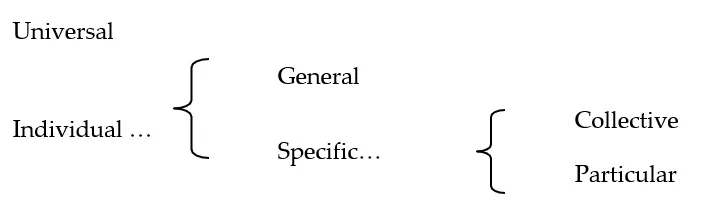
\includegraphics[scale=0.25]{a20220922SacredScience102TheSelfandtheEgo-img001.png} 
\end{figure}

\paragraph{Universals}
This is the medieval understanding of universals:

\begin{quotex}
Universals are those ideas which, while excluding whatever constitutes the difference of things of the same genus or species, represent that which is necessary to their constitution, is essential, and is therefore common to all, remaining fixed in all vicissitudes. Universals are thus merely an expression of those Divine ideas which are concerned with the universal. Universal ideas are opposed to sense impressions, which represent that which is merely individual and contingent in a concrete phenomenon …

\end{quotex}
The highest knowledge is knowledge of the universals. Guenon explains:

\begin{quotex}
metaphysics is essentially the knowledge of the Universal, and such knowledge cannot be enclosed in any formula, however comprehensive it may be.

\end{quotex}
The Universal includes the unmanifested as well as formless manifestation. They are the principles of formal manifestation. Formless manifestation has Being but not individual Existence. The Individual states are all part of formal manifestation.

\begin{wrapfigure}{rt}{0.5\textwidth}
\centering
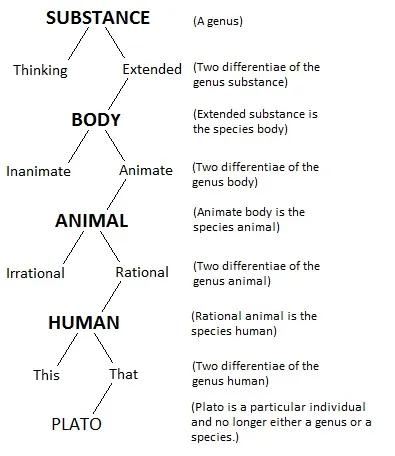
\includegraphics[scale=0.5]{a20220922SacredScience102TheSelfandtheEgo-img002.png}
\caption{The tree of Porphyry}
\end{wrapfigure}

The \textit{unmanifested state} comprises all the possibilities which are not susceptible of any manifestation, as well as the possibilities of manifestation themselves in principial mode. Formless manifestation is not part of multiplicity.

\paragraph{Individual, General, Specific, Categories}

The individual is a state of the Self, of which it is a reflection. It is related to the Universal through a series of genera and species, or the General and the Specific. The individual can only be a species, not a genus. This is illustrated by the Tree of Porphyry.

The unique individual is still not completely defined by the genus and species. There are conditions that makes the individual unique. Aristotle’s categories are genera that characterize the individual precisely. Among these conditions are time, place, qualities, and relations.

Guenon warns about those philosophers who consider the categories as universals. Thus, they will take a quality, such as a color, and try to make it universals. E.g., they will talk about the “idea of redness”, etc.

The being that manifests is necessarily what it is, through its principal manifestation. It is not a matter of chance or fortune.

\paragraph{States of the being}
Another way to look at it, is from the perspective of the states of the being as shown in the diagram in the Fig.~\ref{fig:SacredScience102c}.

\begin{figure}[t]
\centering
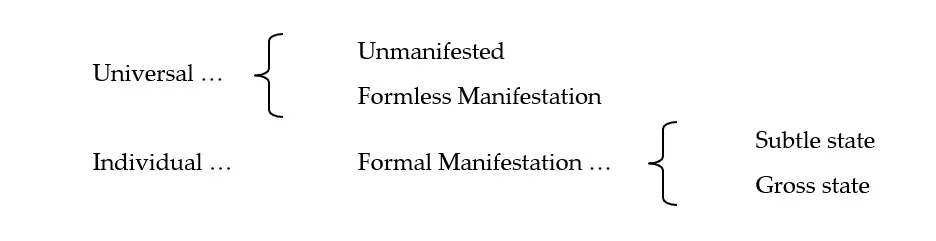
\includegraphics[scale=0.25]{a20220922SacredScience102TheSelfandtheEgo-img003.png} 
\caption{States of being.}
\label{fig:SacredScience102c}
\end{figure}

For the human being, there are two states that comprise it.

\begin{itemize}
\item \textbf{Gross state}: corporeal existence itself, to which human individuality belongs only through one of its modalities. 
\item \textbf{Subtle state}: the extra-corporeal modalities of the human being 
\end{itemize}
Guenon elaborates:

\begin{quotex}
the human being, considered in its entirety, comprises a certain set of possibilities which constitute its corporeal or gross modality, plus a multitude of other possibilities which, extending in various senses beyond this one, constitute its subtle modalities.

\end{quotex}
The modern mind tends to regard the corporeal state as comprising the entire human being, with the subtle states just epiphenomena or otherwise reducible to the gross state.

However, even including the subtle state is inadequate. From the perspective of the Person, the human state is just one state among an indefinite number of other states. That is why the goal of metaphysics is to learn to transcend the human state. Liberation is achieved when all the limiting conditions are overcome.

\flrightit{Posted on 2022-09-22 by Cologero}

\begin{center}* * *\end{center}

\begin{footnotesize}\begin{sffamily}

\texttt{.chris on 2022-09-26 at 18:24 said: }

Is there, if I may humbly require so, canonical yet reasonably concise and systematic literature — regarding the immediate experiential distinction or cumulation of and inner-sense sharpening towards gross and subtle states and sensations and their proper attribution to origin, decoding mere intuition — which earns approval and commendation?

Apart from usually flat and rather ubiquitous reflections of corpo-catalytic alchemical ventures, e.g. tantrik initiate SK Ugranand described — in blog format — in lively, colourful yet clear-cut fashion the phenomenology of amplified subtle and divergent states of being-sensation: waves of energy or unadultered emotion, rhythm-patterned landscapes of feeling and cold cognition, literally analogized consistencies of thought, thought-machines dimensionated and autonomous, layered chronoconsciousness, fed-back archeprimal onomatopoiesis and verging out-towards neuromuscular fine-tuning and proprioceptive decalibration \& on \& on…

Of narrower interest in my regard are aspects of transpersonal commonality, communion and directed/directional empathy and systematic, objectivity-geared lexicalities to wrap and stick around those; since we live in the future of some purported darker past, eager meditations on neurologic hard code elucidated and mirrored by high technology and abetted by — co-emergent? –hypersensitive, hyperassociative deep learning AI are warranted, too… [[yet beware the machinic predator living in cracks of cracked reality microcode — its chronoplasticity beyond bliss, pain and hypnosis is the devils drumming itself]]

Besides, Mr Salvo, please accept my plain gratitude for your work in this rare blog. In certainty, inbetween puzzling my head and easing my soul, the former is the lesser task.

\end{sffamily}\end{footnotesize}

\section{Sacred Science 103: The Vital Center}

\begin{figure}[t]
\centering
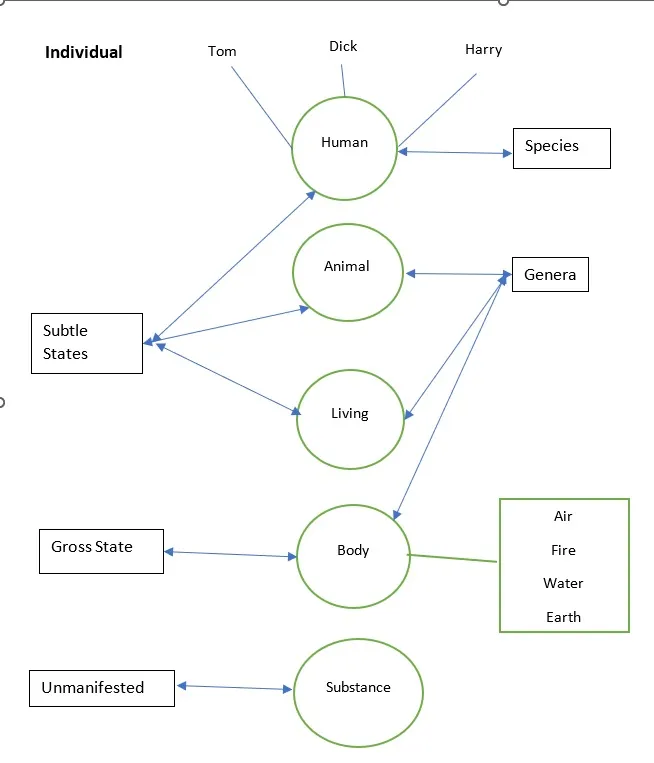
\includegraphics[scale=0.25]{a20220928SacredScience103TheVitalCenter-img001.png}
\caption{The manifestation of the Individuality}
\label{fig:SacredScience103_1}
\end{figure}
 
The diagram in Fig.~\ref{fig:SacredScience103_1} combines the two diagrams from the chapter, \emph{Self and Ego}, that illustrate the manifestation of the individuality. The unmanifested Primordial Substance potentially contains all the possibilities of manifestation. The gross state and the two subtle states are genera, and the human is the species. Particular individuals are manifestations of the species, although with special conditions that make each one unique.

The individual is not yet the Self or Atman, but as jivatman (living soul), it is the particular manifestation of the Self in life. The Atman is identical to Brahman. That identity is called the Supreme Identity, which must be realized (i.e., made real) through the intimate and essential union of the being with the Divine Principle.

\begin{wrapfigure}{rt}{0.3\textwidth}
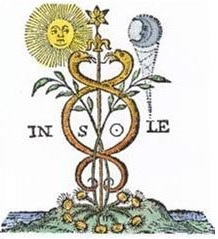
\includegraphics[scale=0.65]{a20220928SacredScience103TheVitalCenter-img002.jpg} 
\end{wrapfigure}
 
Nevertheless, Brahmin, or the Divine Spark, resides in the vital center of every human being, not just for the one who is united or liberated. The heart is the center of life and esoterically refers to the seat of intelligence and not of sentiment. The brain is only the instrument of the mental, i.e., of thought in a reflective and discursive mode. Symbolically, the heart corresponds to the sun and the brain to the moon.

The jivatman is like the image of the Atman, hence it is illusory in relationship to the Atman. The Self is only potentially in the individual, as long as the Union is not realized. However, the Self is not affected in any way by the realization.

\paragraph{Possibility and Potential}
Potential means the aptitude for a certain development and it supposes a possible actualization. It can be applied only in regard to becoming or manifestation. That is because the Self is complete in itself and has no unactualized potential.

But for the individual, all the possibilities that surpass him appear as potential as if he had his own being from himself. What he can attain is actually only a reflection, and not the possibilities themselves. Although this is only an illusion, one can say that these always remain potential for the individual, since he cannot attain them as an individual. As soon as all the possibilities are realized, there is truly no more individuality.


\bigskip

\flrightit{Posted on 2022-09-28 by Cologero}

\begin{center}* * *\end{center}

\begin{footnotesize}\begin{sffamily}

\texttt{Balder on 2022-10-05 at 09:14 said: }

“The two birds that reside in the same tree”, as the Mandokyua Upanishad puts it. I have lately thought about Odinn's ravens Hugin and Munin or the Eagle and the Hawk that reside in Yggdrasil; they might perform the same function of the Self and ego than in the Upanishadic Hindu tradition.

Although I personally see Hugin and Munin representing the left and the right hemispheres of the brain, who's to say they wouldn't have another function as well according to the traditional symbolism and the apparent duality of reason and logic \& imagination (“I Mage Nation”) and emotion. It is also integral to realize that in our bodily functions the left hemisphere guides the right hand and the right hemisphere the left hand.

It is not long ago that I read again Guénon's Man and His Becoming According to the Vedanta and Introduction to the Study of the Hindu Tradition, and there was a lot to ponder concerningthe Atma and jivatma and other correspondences. As I have been delving into the Nordic Traditions for the past 12 years, I have become to see Odinn and Wäinämöinen representing the Self and Loki and Joukahainen the ego, in hindu terms Odinn and Wäinämöinen is the Atman, Atma-Budhi, Christos etc. while other figures of mythology represent the different planetary powers (Thor / Jupiter, Odinn / Mercury, Freya / Venus, Tyr / Mars, Balder / Sun etc). Loki and Joukahainen are as the Norse equivalent of the male polarity of Lucifer or Satan, respectively.

\end{sffamily}\end{footnotesize}
\section{Sacred Science 104: Essence and Substance}

Purusha and prakriti are the two poles of all manifestation.

\textbf{Purusha} is the active principle, represented as masculine.

\textbf{Prakriti} is the undifferentiated primordial substance. It is the passive principle, represented as feminine. It is purely potential and passive, capable of any determination while actually possessing none. Prakriti therefore cannot be a cause by itself (i.e., efficient cause), apart from the action or rather the influence of the essential principle, which is Purusha, and which is the determinant of manifestation.

Universal Being is one, and is polarized. All manifested things are produced by Prakriti, of which they are modifications or determinations. But without the presence of Purusha, these productions would be devoid of all reality. In other words, the productions would be nothing in particular, but rather random variations of the Purusha.

\begin{wrapfigure}{ht}{0.35\textwidth}
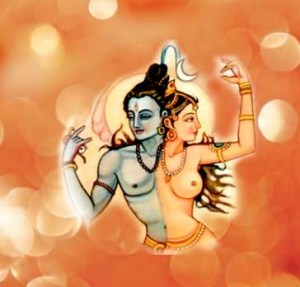
\includegraphics[scale=.4]{a20221006SacredScience104EssenceandSubstance-img001.jpg} 
\end{wrapfigure}

In the West, this teaching is called hylomorphism and has gone by names like “form and matter” or, in Greek, eidos and hyle. Guenon prefers the terms “essence” and “substance”, because if taken in their broadest sense, they provide the most exact idea of the conception in Western languages.

\paragraph{Productions of Prakriti}
Purusha is neither productive nor a production. Nevertheless, Its action essentially determines everything that is substantial production in Prakriti. However, this action is “nonacting activity”.

Prakriti is also not a production, but it is productive. There are seven principles, or productions of Prakriti that give rise to manifestation. These are:

\begin{enumerate}
\item \textbf{Buddhi}. This is the Higher Intellect, which is formless manifestation. Thus, Intelligence is at the beginning of manifestation, so it does not arise randomly from something lower. 
\item \textbf{Ahankara}. This is the ego or individual consciousness brought about by thought. It is the reflection of Buddhi in subtle manifestation. 
\item \textbf{Tanmatras}. These are the essential determinations of things, which are incorporeal and outwardly imperceptible as they are part of subtle manifestation. These include the senses of hearing, touch, sight, taste, and smell. Hence, the possibilities of sensual awareness is prior 
\item \textbf{Manas}. The Mind includes mental functions related to thinking, such as memory, imagination, and common sense. 
\item \textbf{Buddhindriyas}. These are the faculties of sensation associated with the respective tanmatra. As such, they bridge the subtle and gross states. The ear, skin, eyes, tongue, and nose are produced in order to experience the tanmatras. 
\item \textbf{Karmendriyas}. These are the faculties of action such as locomotion, manipulation, reproduction, elimination, and speech. The need for such faculties forms the body. 
\item \textbf{Bhutas}. These are the five substantial and sensible elements which form gross manifestation 
\end{enumerate}
\paragraph{The Three Forces}
Purusha is the ordering principle for Prakriti. There are three forces, called gunas, in Prakriti which are in perfect balance in its primordial state. However, beings, in their various states, relate to these forces in different degrees. These are the three gunas, along with their names in the Western tradition.

\begin{itemize}
\item \textbf{Sattva or Neutralizing Force}: conformity to the pure essence of Being (Sat), which is identified with intelligible Light or Knowledge, and represented as an ascending tendency. 
\item \textbf{Rajas or Positive Force}: the expansive impulse, according to which the being develops in a certain state and, in some way, at a determined level of existence. 
\item \textbf{Tamas or Negative Force}: darkness, equated with ignorance, and represented as a downward tendency. 
\end{itemize}
Beings must strive to keep these forces in balance.

\paragraph{The Human State}
When it comes to the corporeal body in the human state, then matter is, in some way, analogous to Prakriti. We certainly don't count on science to prove anything, but it is appropriate to point out that science is consistent with metaphysics. Here are two major points.

\textbf{Matter is indeterminate}. According to quantum theory, matter is fundamentally indeterminate, being nothing more than probability waves. A thing comes into existence through a collapse of the wave function; how that happens is unknown and is called the “measurement problem”. The Traditional teaching is that a higher intelligence, through non-acting acting, instigates the Purusha to produce forms.

\textbf{Matter has no qualities}. Science advanced when it removed all qualia from its observations. Hence, qualia like color, taste, odor, and sound have no place in science and are not part of any equation. Traditional teaching agrees with this; i.e., the sense arise in consciousness, not in matter. Human consciousness, therefore, participates in the creation of the world by adding sense and intelligibility to it.

Biology today assumes that the organs of sense and action arose accidently through random variations. But why would sense organs arise, and what survival value can they provide, if matter is devoid of qualities? Why would analogous organs of action arise randomly? Traditional teaching is opposite to that, since it teaches that these organs are the result of will. In this extract, Valentin Tomberg summarizes those teachings; those of you on the fence can decide which version sounds more plausible.

\begin{quotationx}
Tentacles, paws, arms, wings — are they not simply diverse forms manifesting a common prototype or principle? They are in so far as they express the desire to bear the sense of touch further, to be able to touch things more removed than those in the immediate neighborhood of the surface of the body. They are active extensions of the passive and receptive sense of touch which is spread out over the surface of the organism. In making use of them, the sense of touch makes “excursions” from its usual orbit circumscribed by the skin which covers the body.

The organs of action are simply crystallized will. I walk not because I have legs but rather, I have legs because I have the will to move about. I touch, I take and I give not because I have arms, but I have arms because I have the will to touch, to take and to give. The “what” of the will engenders the “how” of the action (the organ), and not inversely. The arms are therefore the expression of the will to bear touch further than the surface of one's own body. They are the manifestation of extended touch, due to the will to touch things at a distance. It is similar with wings. They are also an exteriorised will — a will become organ.

\end{quotationx}

\textit{Image courtesy of Hindu website\footnote{\url{https://www.hinduwebsite.com/symbolism/purusha-prakriti-symbolism.asp}}}

\flrightit{Posted on 2022-10-06 by Cologero}
\section{Sacred Science 105: Individual Manifestation}

The \emph{Bhagavad Gita} mentions three Purushas.

\begin{enumerate}
\item \textbf{Jivatman}. This is human Individuality and is destructible. 
\item \textbf{Atman}. The indestructible Self or the Personality. 
\item \textbf{Paramatman}. Spiritually identical to the absolute and ultimate reality 
\end{enumerate}
\paragraph{Vertical Causation}
Purusha is the essential (or efficient) cause and Prakriti, the substantial (material) cause of all manifestation. Prakriti contains in potential all the possibilities of manifestation while Purusha determines the development of the possibilities of Purusha thought their passage from potency to act.

In the West, Prakriti is analogous to Prime Matter, at least insofar as it concerns the human state. Hylomorphism is the process by which prime matter (potency) is individualized by an immaterial essence (act).

Of course, matter, as physicists think they understand it, is not what is intended by Prime Matter. Nevertheless, when physicists reach the foundation of matter, they don’t discover things but rather probability distributions described by a wave function, i.e., potency without act. How things come into existence is an inexplicable mystery; that is the so-called “measurement problem”. But physicists have no understanding of Purusha or Prakriti because, as unmanifested, they cannot be measured no observed. Hence, that mystery will never be solved.

\paragraph{Jivatman}
Ahankara is the ego or individual consciousness brought about by thought. Hence, Descartes could explain, “I think, therefore I am!”

The ego is the reflection of Buddhi — part of formless manifestation — into subtle manifestation. The ego is the reflection of the Atman on the soul, like the way sunlight is reflected onto water. Hence, it appears identical to the Atman which gives it birth. The quality of the image depends on the stillness of the water; hence, the freer the soul is from perturbations and undulations, the better will be the reflection of the Atman.

\paragraph{Microcosm and Macrocosm}
If Paramatman represents the Macrocosm, then jivatman is the microcosm. The ego may seem to be one, but careful self-observation reveals it to be multiple. One day, you make a resolution and break it the next day. One day you are happy and then anxious. These represent little I’s that contend for a small part of conscious life.

This is seen more clearly in the dream state. In a dream, or even lively fantasies, jivatman is creating all the characters while believing that they each have a life of their own.

Just as Atman develops all the possibilities of manifestation, the jivatman develops all the possibilities of the individual human state.


\textit{This is tied to Chapters 5 \emph{Purusha Unaffected by Individual Modifications} and 6 \emph{Degrees of Individual Manifestation} from \emph{Man and his Becoming}.}

\flrightit{Posted on 2022-10-13 by Cologero}
\section{Sacred Science 106: Origin of Mind}

Being is One, yet it contains within itself multiplicity, since it produces it by the deployment of its possibilities alone. Purusha (Essence) and Prakriti (Substance) are the two poles that bring these possibilities into manifestation.

Prakriti contains all possibilities of manifestation as known by Purusha, so it is the first principle of manifestation. Prakriti is passive and purely potential so that it cannot be a cause in itself. That means that intelligence comes prior to any sort of manifestation.

\begin{figure}[t]
\centering
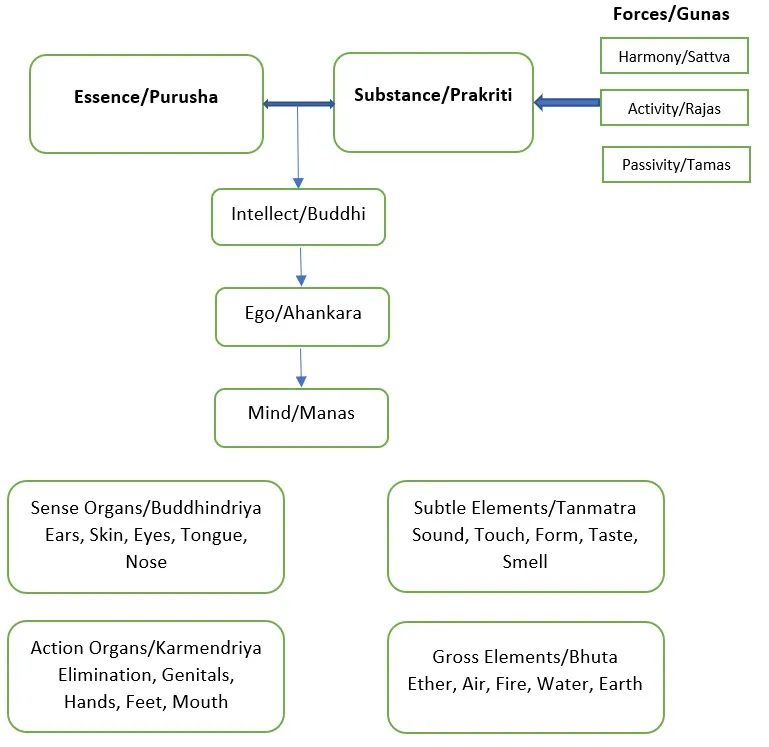
\includegraphics[scale=.35]{SamkhyaChart.png}
\caption{Samkhya Chart}
\end{figure} 

In Western terms, Purusha is Essence and Prakriti is Substance. The union of Essence and Substance is called hylomorphism. This is not dualistic in the Cartesian sense. Rather it recognizes that there is both an inside and an outside to the world, the former as the subtle state and the latter as the gross state. The understanding of the multiple states of the being avoids philosophical conundrums like explaining the relationship between consciousness and matter, or how they interact.

\paragraph{Intellect}
The first production of Purusha and second principal is the Intellect (Buddhi). Although manifested, it is formless.

Thus, there cannot be any direct experience of it. The Intellect is of a transcendent order and has the knowledge of universal principles as its proper object. This knowledge, which is not discursive, is obtained directly and immediately by intellectual intuition.

There are stories about direct intuition of the Intellect. For example, mystics, composers, poets, philosophers, visionaries, etc., have often reported that their greatest works just “came to them”, as if from the outside. The mathematician, Ramanujan, claimed that a goddess revealed all his mathematical discoveries to him. Their task, then, was just to write down their inspirations.

Perhaps, you’ve had a similar experience on a smaller scale. Often that is called the “aha experience”. Suppose you have been working on a mathematical problem without understanding, but then suddenly you just “get it”.

\paragraph{Ego}
The Intellect is the intermediary between personality and individuality. The formless Intellect produces the individual consciousness, or the Ego. As the essences in the Intellect give rise to thought, evoking the notion of the Ego or “I am”.

The Ego becomes concerned with external and internal objects, which are respectively the objects of perception and of contemplation, or in other words, the subtle states and the gross state.

\paragraph{Mind}
Mind, or Manas, is related to individual thought, including reason as well as memory and imagination. In the West, this includes the Five Wits: memory, estimation, fantasy, imagination, and common sense.

The Mind is part of the subtle realm, yet it is the intermediary between the organs of sensation and action. The lowest part of the mind is involved with the senses and the organs of action.

\paragraph{Organs}
These organs allow the human being to both sense and act upon the world.

The Sense Organs or Buddhindriyas are produced in order to experience the subtle states. For the human being, these are the Ears, Skin, Eyes, Tongue, and Nose. They correspond to the senses.

The organs of action are the Karmendriyas. These are the faculties of action such as execratory organs, reproduction, manipulation, locomotion, and speech or ingestion. These are general conditions of life and are found in almost all forms of animal life. For the human being, they are the anus, the genitals, arms, legs, and mouth.

\paragraph{Subtle Elements}
The subtle elements, or Tanmatras, are Sound, Touch, Form, Taste, and Smell. Together they form the inner experience of the world.

Although these are not experienced outwardly, that does not indicate that they are merely subjective experiences. They are as much a part of the world as are the gross elements.

\paragraph{Gross Elements}
The gross elements, or bhutas, are ether, air, fire, water, and earth which correspond to the subtle experiences: auditory, tangible, visible, sapid, and olfactory.

Note that the gross elements are the very last productions of prakriti. Together, they form what is called “matter” by science and in common usage. The material world, in itself, does not have any sensible qualities. Galileo made it explicit: secondary qualities (such as sense experience) are not part of science. For example, all the theories and equations of science do not require the notion of color, nor any other subtle element.

For science, matter is characterized by number, extension, solidity or mass, and motion. The subtle elements are the principle of the gross elements, but matter is the principle of multiplicity. In matter, there can be multiple instances of the same essence.

Ether can also be understood as space, so matter has extension in space as well as shape.

Earth represents mass and fire the energy associated with motion. Air and water round out the other states of experienceable matter.

Since matter is closest to Prakriti, it takes on some of its characteristics. For example, matter includes three forces, usually expressed by the terms positive, negative, and neutral.

Prime matter, similar to Prakriti, is passive and malleable. Quantum indeterminacy is analogous to the receptivity of Prakriti. Vertical causation, i.e., the influence of Purusha on Prakriti ends indeterminacy so that individual things are formed.

Profane science believes that the matter of the gross state is fundamental and so that all the productions are caused by matter. This includes the senses, the mind, thoughts, the Ego, and Intelligence. Random evolution brings the organs of sense and activity into existence. But if matter has no secondary qualities, what is the purpose of the evolution of the eye to “see” something that simply isn’t there?

The scientific view implies that all the possibilities of manifestation are hidden in matter somewhere. There is certainly no compelling reason to believe that and no physical theory can explain it.

Some claim that “emergent evolution” offers an explanation, but that just means that there must be something higher than matter, in order for new qualities to arise.

\flrightit{Posted on 2022-10-27 by Cologero}

\begin{center}* * *\end{center}

\begin{footnotesize}\begin{sffamily}

\texttt{Rui Artur on 2022-10-28 at 10:03 said: }

It might be useful to note in the text – for those who wish to go forth and link this to the Western Tradition – that in texts from the Latin part of the world one will encounter the idea of Purusha coming from the Greek ousia but translated as ‘substance’ (rather than ‘essence’). This can cause some confusion if one is not reading carefully or just beginning his study, even though ‘essence’ is etymologically correct and substance is not (which is why I think Guenon used it).

\hfill

\texttt{Balder on 2022-10-30 at 09:57 said: }

I have related the Nordic conception of Ginnun-Ga-Gap as the Absolute (greek Khaos) and Fire representing Essence/Purusha and Ice Substance/Prakriti. There is a fine thread uniting Hindu metaphysics, indo-European Cultural connexion and Norse / Finno-Ugric / European Pagan metaphysics.

\hfill

\texttt{Balder on 2022-10-30 at 10:03 said: }

In the Finno-Ugric tradition the same concepts are Lintukoto (The Birdlands) and Pohjola (The Northlands).

In the Norse tradition the trinity Odin-Vili-Ve represent the threefold structure of buddhi-ahamkara-manas.They are the “first creator Gods” to emerge from the primordial chaos and they slay Ymir, who is here Purusha personified. Essence is “slayed” or crucified into the Cross of matter.

\hfill

\texttt{Cologero on 2022-10-31 at 17:14 said: }

This is a work in progress, and some things, particularly terminology, will have to be reviewed.

\hfill

\end{sffamily}\end{footnotesize}
\section{Sacred Science 107: The Heart of the Matter}

Three physicists walk into a bar … I mean, they participate in a panel discussion about the existence of the multiverse. There was one for it, and two against, with three different perspectives

\textbf{Michio Kaku} has become a science popularizer and is on the physics fringe with string theory, belief in alien visitations, and outlandish claims about the benefits of quantum computing. He claims that the multiverse explains quantum theory, but offered no way to test it in a scientific way. But hyperbolic predictions make for engaging pop science.

The human being, in Kaku's perspective, is just an assemblage of matter. A copy of a human being — with all its memories, hopes, dreams, plans — can be instantly created, just from matter, and just because an electron somewhere was “measured”. It is analogous to a human version of mitosis.

\textbf{Sabine Hossenfelder} has also become a popularizer with an often useful youtube channel. She is a materialist and believes in something called superdeterminism, i.e., everything that happens is predetermined. She suspects that there are hidden variables that would overturn the apparent randomness of quantum events. They are still hidden.

Presumably, those variables, hidden away since the Big Bang, can account for all the motions and activities of a typical day in New York City.

\textbf{Roger Penrose}, who is actually a mathematician, is a Platonist. He is convinced that there is a fundamental flaw in quantum theory. I vote for the Platonist. Obviously, if a physical theory gives rise to several incompatible “interpretations”, then it is at best incomplete.

So what to do when three eminent physicists find themselves in a Mexican standoff\footnote{\url{https://en.wikipedia.org/wiki/Mexican_standoff}}? A clue came from the astute question about the efficacy of physics: why is the world intelligible at all? They were taken aback by the question, with one claiming that it is just a “given”. Well, then who or what “gave” it?

\begin{wrapfigure}{rt}{.4\textwidth}
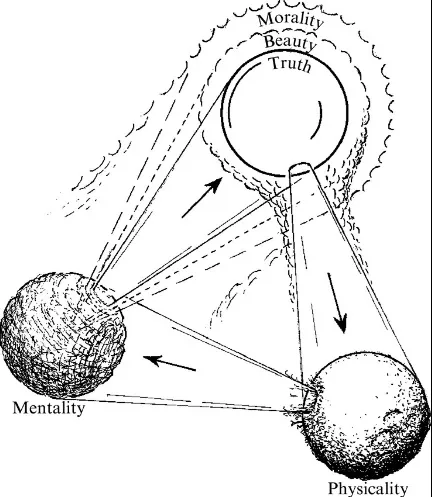
\includegraphics[scale=.35]{a20221106SacredScience107TheHeartoftheMatter-img001.png} 
\caption{Road to Reality}
\end{wrapfigure}

Penrose, in his book \emph{The Road to Reality}, came to the conclusion that there are three worlds, only one of which is amenable to physics. In his earlier works, the diagram that illustrates the Platonic realm of Truth, Beauty, and Morality only included Mathematics. From the Platonic perspective, Mathematics is in between the realm of ideas and the physical world. In his diagram, only Truth is related to the physical world. Penrose has enough self-awareness to recognize that any discussion of beauty or morality has no physical explanation; they make sense only in the mental world.

As for the mental world, he recognizes that any universe that can be observed requires the existence of conscious observers. This requirement places many constraints on the physical world in order for conscious beings to exist at all. This is a version of the Anthropic principle even if no one currently knows all the constraints.

\paragraph{Gross manifestation}

\begin{figure}[t]
\centering
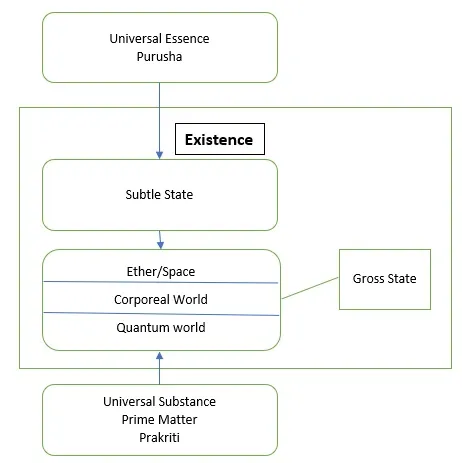
\includegraphics[scale=.5]{a20221106SacredScience107TheHeartoftheMatter-img002.png} 
\caption{World of Things}
\end{figure}

This segues into traditional metaphysics. In this diagram, existence consists of the subtle state and the gross state, which Penrose calls mentality and physicality. In the next installment, the subtle state will be further broken down, but at this point, only the gross state is being described.

\paragraph{Corporeal World}
The Corporeal World is that of our everyday experience, symbolically represented by the elements of Air, Fire, Water, and Earth. This is the world studied by science. Ever since Galileo, at least, science eliminates the sensible experiences of sound, sight, touch, smell, and taste. They belong to the subtle state, or mentality. No fundamental theory of science requires mentality.

As purely physical entities, the science of the corporeal world deals with count, shape or extension, mass, and motion or energy.

\paragraph{Space}
The element Ether is also called Space. It is the bridge between gross and subtle manifestation, since space does not exist in the subtle realm. Although you can pick up a rock, or drink water, you cannot find a piece of space. Nevertheless, space is part of gross manifestation because it is actually formed by matter. In other words, things don't exist in space, but their very existence is space. General relativity demonstrates that a massive distorts the local space around it.

\paragraph{Quantum World}
Physics was motivated to find the smallest unit of matter, which was called the Atom. At first, it seemed successful when the basic elements were organized into the Periodic Table. But as physics kept probing, even more elementary particles were discovered. Ultimately, with quantum theory, there was nothing in particular, just potentiality as described by Schrödinger's Equation. The corporeal world arises when something is measured; what that entails is still not clear to physics. Thus, various interpretations of quantum theory have been proposed to account for it.

Wolfgang Smith has asserted that, with the quantum world, physics has discovered a plane of existence between the traditional Prime Matter and the Corporeal World. That is plausible, since it has characteristics of Prime Matter, yet is physically observable.

\paragraph{Possibilities of manifestation}
If, as physicalists believe, everything that exists arises from the measurement problem, then the existence of things, life, consciousness, and thought must somehow be hidden in Schrödinger's Equation. To date, no one has offered any plausible physical explanation for consciousness or rationality. Yet they are as observable as anything else; actually, the physicist himself illustrates it.

The alternative is to believe in emergent evolution, which is the theory that entirely new properties can arise over the course of time. Obviously, that theory has its own problems, such as explaining the origin of such properties.

In traditional metaphysics, Universal Substance or Prakriti is pure potentiality. All the possibilities of manifestation reside in it. The quantum world is the bridge, then, between Prime Matter and the Corporeal World.

In particular, there is absolutely no physical explanation of the human being. A human being loses and gains matter at every moment, yet the being persists across time. Personal experience demonstrates it. This rules out any multiverse theory. There cannot be a counterpart of a human being in another universe. There is clearly no personal continuity.

\paragraph{Intelligibility}
Now we return to the question of the intelligibility of the world. This requires something that transcends the physical world as Penrose noted. The Essence or Idea of things resides in Purusha. Things are known because the idea of the thing is known. Otherwise, the thing is a mere assemblage of atoms, with the same lack of inherent intelligibility as a mound of windblown sand on the beach.

For those who are time constrained, just listen to the three minute introductions of the three panelists in this video: 

\url{https://youtu.be/W39kfrxOSHg}.

\flrightit{Posted on 2022-11-06 by Cologero}

\begin{center}* * *\end{center}

\begin{footnotesize}\begin{sffamily}

\texttt{veritycacciatrice on 2022-11-07 at 10:10 said: }

“The alternative is to believe in emergent evolution, which is the theory that entirely new properties can arise over the course of time. Obviously, that theory has its own problems, such as explaining the origin of such properties.”

Surely the same properties are always here, appropriate to this world, but the knowledge becomes lost or misinterpreted through time. Humanity cyclically falls like a sack of spuds.

But some mythologists- in describing things that *do* happen- knew eventually civilisation would get back to a certain state of consciousness and technological competence, as it always will, at which time things steeped in dim and boring obscurity, like say… oh I don’t know, the bible for example, suddenly becomes an extraordinarily lucid metaphysic-consciousness handbook almost overnight.

`It’s not just the Big Bang and general relativity that is in trouble, but the foundation of them all.

Gravity is an exhausted and bankrupt concept. A higher, more comprehensive concept is needed. The technologies of gravity have lifted us to a viewpoint that is bigger than gravity.

We need new ideas and new tools such as the Electric Universe model to make sense of the new plasma vistas.’

-Mel Acheson, author of this $>$10min. post from Thunderbolts Project;
\url{https://www.youtube.com/watch?v=dBBJyXwFjWQ}

Note: it is a model, that is, it can be modelled from the lab to cosmic dimensions. Not a theory. 

And on the special bonus plan; `What is Light?’

\url{https://www.youtube.com/watch?v=SZ5ZWbVWMBU}

The question at the end is, what moves? It can only be the consciousness of the observer, which is about as `quantum' as it needs to be.

As an aside, `quantum' is `how much' in Latin.

It’s as if they’re asking us, `How much theory' can you people take until it all blows apart and reality kicks back in.


\hfill

\texttt{Balder on 2022-11-08 at 14:22 said: }

The taichitu explains in a perfectly simple Manner how in manifestation there can never be substance without essence and vice versa.

\hfill

\texttt{Ignatius on 2022-12-26 at 17:06 said: }

It is to be recalled the notion of the `reversal of space and time' as a sign of the times acknowledged in Guénons `Reign of Quantity' and one might notice the apparent significance of the notion of the `event horizon' that has arisen within contemporary mathematical frameworks: as the separation between the environments within and outside an event horizon is marked precisely by the reversal of spatial and temporal components of any trajectory that crosses both environments. As `space' changes into `time', the `event horizon' becomes the trajectory’s `past' and thus cannot be crossed; time changes into space making the `event horizon' a spatial symbol for the separation of `past' and `future' of our perspective. 

The `Reign of Quantity' thus manifests itself in two ways: The discovery (or rather `descent into') a chaotic interim realm between `materia prima' and the corporeal world on the one hand, and the obscure abode of Janus that is the `event horizon' on the other hand; it is to be considered thus not only a spatial symbol of the `end times', but also of `initiation'; a correspondence which should hardly be surprising if one understands the principles underlying the cycle of manifestation.

The truth of this observation is independent of the question whether the mathematical `modes' by which these realities are formulated have any merit whatsoever; the symbolic correspondence is comprehensible inasmuch as they appear in the universal descriptions of the people in this age.

\end{sffamily}\end{footnotesize}
\section{Sacred Science 108: The Subtle State}

The Self or Atman, manifests itself as a soul (jivatman) in the living form of the individual human being. It is covered in a series of successive sheaths, or koshas, representing phases of its manifestation.

I am associating the koshas with names of bodies, even thought, apart from the physical or gross body, are not really bodies. Moreover, the names are for convenience and are not tied to any particular school or organization.

Note that one sheath is associated with the spirit or pneuma, and one with the body or soma. There are three associated with the soul or psyche.

\begin{enumerate}
\item \textbf{Anandamayakosha or causal body}: This is the set of all the possibilities of manifestation that Atman contains in itself. It is unconditioned and formless. In relation to the formal manifestation, it is the causal form through which the human being will be manifested and actualized. 
\item \textbf{Mananayakosha or Mental Body}: This sheath is formed by the intelligible Light of universal Knowledge. It consists in joining the superior intellect (Buddhi) to the tanmatras. 
\item \textbf{Manomayakosha or Astral Body}: This includes the mind (manas) and all its activities. 
\item \textbf{Pranamayakosha or etheric body}: This includes the vital breath (prana) and is modalities (vayus). It also includes the faculties of sensation (Buddhindriyas) and of action (karmendriyas). 
\item \textbf{Annamayakosha or gross body}: This is the physical body. It assimilates food to keep the body operational. 
\end{enumerate}

\paragraph{Laws}
At each level, the human being is subjected to increasingly strict laws.

\begin{itemize}
\item \textbf{Causal body}. Since this is unconditioned, it is liberated from all laws and conditions. 
\item \textbf{Mental body}. It is subject to all the laws of thought including logical and mathematical laws. 
\item \textbf{Astral body}. The human being is subject to psychological laws. 
\item \textbf{Etheric body}. The human being is subject to all the biological laws of the system. 
\item \textbf{Gross body}. The physical body is subject to physical and chemical laws. 
\end{itemize}

\paragraph{Subtle State}

Since we already described the gross state in Sacred Science 107: The Heart of the Matter, and will deal with the unconditioned state at a later time, this section will deal with the subtle state.

This requires a more refined description of the three sheaths. There are two factors that need to be considered:

\begin{wrapfigure}{rt}{.35\textwidth}
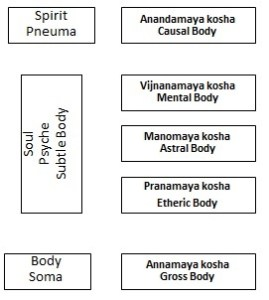
\includegraphics[scale=.5]{a20221113SacredScience108TheSubtleState-img001.jpg}
\caption{The Koshas/Sheaths}
\end{wrapfigure}

\begin{itemize}
\item Like all manifestation, the sheaths are subject to the gunas. Therefore, each sheath has a negative part, a positive part, and a neutralized correlate. 
\item The sheaths are not entirely independent because of the unity of the being. Therefore, the divisions are not sharp, so they blend into each other. These are represented by sectors within the center. 
\end{itemize}
Instead of sheaths, we can regard them as centers within the being. These are the intellectual, emotional, and motor centers, corresponding to the second, third, and fourth sheath respectively.

Note that each center is divided into a positive and negative part (above and below the line).

Because of the interaction of the centers, thoughts, feelings, and actions are seldom pure. Everything is mixed and even entangled. For example, we may not think honestly because our emotions cloud our judgment. Or false intellectual ideas can affect the emotions, causing pleasant emotions from bad ideas.

\paragraph{Intellectual Center}
This center is the focus of discursive thought. It analyzes, calculates, and so on. There is the ability to understand mathematics and logic. The gnomic will, which deliberates alternative courses of action, is also part of this center.

Creative ideas arise from the positive part of the intellectual center, while criticisms come from the negative part. When they are in balance, the creative idea will improve from a critique. But often the negative part will thwart the idea. Irrational and illogical thoughts can also arise from the negative part.

\begin{wrapfigure}{rt}{.35\textwidth}
 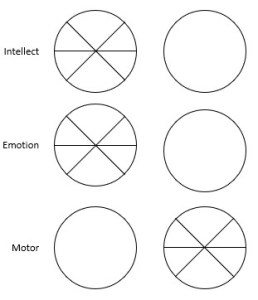
\includegraphics[scale=.5]{a20221113SacredScience108TheSubtleState-img002.jpg} 
 \caption{Centers of Subtle Body}
\end{wrapfigure}

Mechanical thoughts come from the motor sector of the intellectual center. They arise spontaneously. People will just repeat the same comment, often absorbed through propaganda, whether pertinent or not. It is impossible to have an intelligent conversation with someone who thinks mechanically.

The emotional sector will distort thoughts. A strong emotion will usually lead to thinking that justifies the emotional reaction, without any basis in fact.

If one succeeds in neutralizing or reconciling the thinking center, the higher thinking center can arise. That is represented by the circle without a positive and negative part, and without sectors.

\paragraph{Emotional Center}

The is the center of feelings, refined sensations, passions. The stream of consciousness of thoughts and images arise here. If the negative part of this center is in harmony, it completes the positive part. For example, positive emotions are associated with agreeable things and negative emotions with the disagreeable.

But too often, negative emotions like anxiety, depression, anger, fear, and so on come to dominate. This distorts the entire life of the human being. This is verified end by secular standards. That is why esoteric training emphasizes the emotions so much. Again, there is a higher emotional center that can arise by reconciling the positive and negative parts.


\paragraph{Motor Center}
The senses comprise the positive part of the motor center and the negative part includes the faculties of action. Being mostly subconscious, the motor center is the best functioning center in most human beings. It is important to keep it as healthy as possible.

The sexual center is represented by the undivided circle. However, the purification of the sexual center is a discussion for another time.

\flrightit{Posted on 2022-11-13 by Cologero}

\begin{center}* * *\end{center}

\begin{footnotesize}\begin{sffamily}

\hfill

\texttt{Logres on 2022-11-19 at 18:55 said: }

This elucidates with precision and insight. In particular, the statement that balancing the negative and positive parts of a center leads to the arising of the pure center, was creatively well put, and sheds more and more light. This connects practical experience of purification with the somewhat more abstract and mysterious teachings in Mouravieff's work, about higher centers, and ties it into the Gunas. I'm constantly amazed at the connections you make, and find myself more than several steps behind. God speed all your endeavors.


\hfill

\texttt{Dimitri on 2022-11-20 at 18:31 said: }

Both yourself and Cologero have done a great service to us all, Logres. I truly appreciate both of your insights, your posts are always a pleasure to read. This site is full of so many gems, there's no other site out there like Gornahoor.

\end{sffamily}\end{footnotesize}
\section{The Descent of the Absolute}

In \emph{Man and his Becoming}, \textbf{Rene Guenon} describes the manifestation of the Self into the human state according to the Vedanta. The West has its own Traditional understanding. It is not different, but it is worth the trouble to redo the same project in more Western terms. This post can be the barest outline, and specific topics will be developed in future posts.

By the Absolute, we mean generally what is called Brahman, that is, whatever is beyond being. The Self (Atma) is the principle of the individual. As such, the Self is beyond all manifestation and time. The descent through the degrees of being begins with formless manifestation, then to formal manifestation in the subtle state and ultimately to the gross state. This is not a process that occurs in time. Nor does the Self descend through these stages, since it is their principle.

\begin{wrapfigure}{rt}{.35\textwidth}
 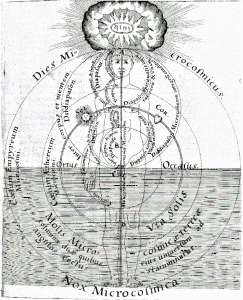
\includegraphics[scale=.5]{a20210307TheDescentoftheAbsolute-img001.png} 
\end{wrapfigure}

A difficult notion to accept is that “time”, as we know it, is a feature of the human state. Once understood, however, many fruitless philosophical and theological conundrums are resolved.

The human state is said to be “rare”, in the sense that it is just one possible state out of many. The situation of the being in the human state allows the being to act in a way to acquire knowledge, unlike other states that are passive. Thus, it is special and should not be squandered.

These are the primary degrees although each one can be further divided, potentially indefinitively, into subdegrees. The Self becomes conscious of the world of sensible manifestation through:

\begin{itemize}
\item Thought 
\item Inward senses or wits 
\item Individual consciousness 
\item Five senses 
\item Five organs of action 
\item Life force 
\end{itemize}
\subsection*{Buddhi}
The buddhi, Universal Spirit, or Higher Intellect belongs to the realm of formless manifestation. As such it is the first degree of the manifestation of the Self. The possibilities of manifestation become ideas or essences in the Higher Intellect.

It is the principle of the formal manifestation of the Self and thus is the unifying principle. Rene Guenon calls it the “Spiritual Sun which shines at the center of the entire being.” Put another way, it is the “spark of divinity,” even if only virtually.

Thought is the faculty which gives form to ideas and associates them to each other; thought is how we experience the Higher Intellect.

However, in the Higher Intellect, it is not yet individual consciousness.

\subsection*{Manas}
The characteristics of the Manas, or Universal Soul, relate to faculties of the formal order.

Mental faculty or inward sense. Individual thought, memory, imagination

\begin{itemize}
\item\textbf{Five elements}: Ether, air, fire, water, earth
\item\textbf{Five Senses}: sight, hearing, smell, taste, touch
\item\textbf{Five Wits}: memory, estimation, fantasy, imagination, and common sense
\item\textbf{Five actions}: Ingestion, excretion, reproduction, locomotion, grasping
\end{itemize}

From the esoteric perspective, the senses are prior in the ontological sense. Moderns believe that somehow matter is creating sensations in the brain. The same for the other features. The desire for locomotion and grasping, for example, direct evolution. They are not the serendipitous results of a random evolutionary process.

Also, the ideas of the elements determine gross manifestation, not the other way around.

\subsection*{Causal Body}
The causal body is the dividing line between pure Being and the individual being. As such, it is the essence of the human being, that is, what he is born with. Boris Mouravieff explains it as analogous to the unfolding of a movie film:

\begin{quotex}
Each human being, then, is born with his own particular film [destiny]. This represents the field of action in which man is called to apply his conscious efforts. 

\end{quotex}
The causal body is still in the formless order. Rene Guenon describes it as

\begin{quotex}
the totality of the possibilities of manifestation which Atma comprises within itself, in its permanent actuality in the principial and undifferentiated state. [It] enjoys the plenitude of its own being, and it is in no way really distinct from the ‘Self’; it is superior to conditioned existence, which presupposes it, and it is situated at the level of pure Being. 

\end{quotex}
But when viewed in relation to formal manifestation,

\begin{quotex}
it can be said to represent principial or causal form, that by which form will be manifested and actualized in the succeeding stages. 

\end{quotex}
Hence, it is the

\begin{quotex}
principle and cause of all manifestation and the source from which manifestation is developed in the multiplicity of its different states and more particularly, as concerns the human being, in its subtle and gross states. 

\end{quotex}
The principles and causes are described below.

\paragraph{Non-dual awareness}
At the level of Being, the causal state is non-dual awareness, beyond the subject-object distinction. As such it creates the sensible world through the three forces:

\begin{enumerate}
\item \textbf{Active force}: The idea or essential cause. This makes the world intelligible. 
\item \textbf{Passive force}: Matter or substantial cause. Matter is the principle of multiplicity. It is pure quantity without any qualities. 
\item \textbf{Neutralizing force}: Consciousness. 
\end{enumerate}
When the horizontal substantial cause meets the vertical essential cause, the thing arises. Yet it is not real unless and until there is consciousness. In the causal state, the virtual senses of the manas are actualized so that the world of the senses — or corporeal world — arises.

Yet there is no separation between subject and object, Self and the world. The self is said to participate in the world because there is no distinction.

\paragraph{Categories}
The categories of being are the most general of all genera and determine the essence of the human being at birth. One's essence is unalterable. The tendency today is to regard these categories as arbitrary, inessential, and even unjust. However, they make the being unique and distinct from other beings. Aristotle's categories are helpful to understand this. Here are some examples.

\textbf{Substance}: Obviously, in this case, the substance is to be a human being.

\textbf{Time and place}: The human being is born at a particular time and place.

\textbf{Qualities}: The human being is born with certain qualities. These include the following, although it is unnecessary to specify precise details, which the reader can easily do.

\begin{itemize}
\item Habits and Dispositions 
\item Natural Capabilities and Incapabilities 
\item Affective Qualities and Affections 
\item Shape 
\end{itemize}
\textbf{Relations}: this includes all the relationships that the being is born into. Among them are parents, family, nation, race, religion, and so on.

\textbf{Sex}: Sex is not a substance because both male and females are fully human, and not different species of the genus “human”. Nor does sex fit into a category of being, as the difference is above a category. Nevertheless, sex is not conventional, nor simply biological. Nevertheless, sex is “constitutive for the person” not an “attribute of the person”.

\paragraph{Messengers of Gods}
In the Divine Comedy, Dante describes the ascent through the planetary spheres and the hierarchy of angels. In the descent of the being, the angels and celestial objects play a role in the progressive manifestation of the being.

The angels mediate the stages of manifestation. In a moral world, there needs to be an adversary, which makes evil a possibility of manifestation. Hence, there are fallen angels that distort the process.

\paragraph{Macrocosm}
The Microcosm is the Macrocosm is a truism in Hermetism. This must, however, be understood in its interiority, not as material forces and objects. This is the true astrology: the Spheres of Heaven correspond to aspects of our soul. Thus, there is the Moon of the being, Venus of the being, and so on. The effects of Mercury, Venus, Mars, Jupiter, and Saturn, understood in their interiority, on our lives need not belabored here.

\paragraph{Archetypes}
Besides the archetypes which manifest from above, there are also

\begin{quotex}
the archetypes which manifest themselves endlessly in history and in each individual biography — they are mythological symbols pertaining to the domain of time. (Valentin Tomberg) 

\end{quotex}
For examples, the prophets can be understood that way: there is the Adam of the being, Noah of the being, Abraham of the being, and so on. Here only Adam concerns us, for the others are part of the re-ascent.

Adam is the father of all humankind. Due to that, we are born in a condition of ignorance, malice, concupiscence. This separates the human microcosm from the purity of the macrocosm. These conditions are not part of the being's essence, because they can be altered and overcome in life. Hence, any attribute or quality that is sinful cannot be an essential part of the human being.

\subsection*{Ego}
Thinking separates the nondual awareness of the causal state into subject and object. At this stage individuality is realized. Thought creates the idea of the Ego experiencing objects “out there, right now”. So Rene Descartes’ quip, “I think, therefore I am,” is exact, presuming that it refers to the Ego of the human state, not the Real Self. The Ego in the individual state forgets its true identity.

\subsection*{Subtle Body}
The human being manifests as a subtle body and a gross, or physical, body. These correspond respectively to two of the conditions of manifestation: psyche (or life) and matter. So in addition to the features of the human being acquired from the vertical direction, he is also subject to the psychical and material currents active in the time and place of his birth.

The subtle body is further subdivided in three: the intellectual, animal (or emotional), and vegetable souls. The soul divisions are porous, so there are no hard divisions between them. Features of each can appear in the others. That is why animals can display intelligence or why a human can feel pleasure in intellectual attainment. More often, the mixture is deleterious. Mouravieff makes that clear:

\begin{quotex}
In fact, we have neither a pure thought nor a pure feeling: nor are our actions pure. Everything in us is mixed and even entangled, often by all sorts of considerations which either come from the intellectual centre, tarnishing the purity of our feelings by its calculations, or from the emotional centre, which clouds the calculations of the intellectual centre. 

\end{quotex}
Since this topic has been covered numerous times, we just need a cursory mention here. A full explanation would require a book.

\begin{itemize}
\item\textbf{Mental Body:}
Intellectual soul Activities related to thinking. The lower part includes opinons and discursive thinking. The higher part is intuitive thinking.

\item\textbf{Astral Body:}
The Sensitive soul or animal soul is the center of the lower mental functions, emotions, feelings as well as refined sensations and passions;

\item\textbf{Etheric body:}
Also known as vegetable soul or life body. This is the center of the faculties of action and sensation, which relate to the corresponding features of the Manas.
\end{itemize}

It also directs unconscious processes like nutrition, growth, secretion, and reproduction.

The motor centre governs instinctive life as well as movement and all mental activity: its action is thus distributed throughout the physical body.

\subsection*{Gross Body}
Matter is not productive of anything. It is only alive when animated by the etheric body. When that latter separates from the gross body, the body dies and decays.

Even the gross body has levels: first, it is subject to the laws of physics, then those of chemistry, and finally biology.

Nevertheless, The qualities of the human being are determined ontologically prior to biological processes. Hence, biology does not create the human being, but rather the other way around.

Nevertheless, the gross body is the medium through which one's destiny is played out. The physical world is the unconscious of the Self.

\subsection*{Level of Being}
A fundamental principle is that what is ontologically prior comes after in time. Hence, at the level of the gross body, it appears that life (etheric body) follows matter, then consciousness, and eventually thought. In the temporal sense, the world appears to “evolve” from the lower to the higher.

However, ontologically there is no absolute standard of time, so the states are, from the viewpoint of the Self, simultaneous. Where the Self “is” in the states of the being is determined by where the Self is focusing consciousness.

\subsection*{Sources}

\textsc{Barfield, Owen}: \emph{Saving the Appearances}

\textsc{Dante}: \emph{Divine Comedy}

\textsc{Guenon, Rene}: \emph{Man and his Becoming according to the Vedanta}

\textsc{Lewis, C. S.}: \emph{The Discarded Image}

\textsc{Shankara}: \emph{Tattva Bodhah}, Commentary by Swami Tejomayananda

\textsc{Shankara}: \emph{Vivekacudama\d ni}, Commentary by Swami Dayananda Saraswati

\textsc{Mouravieff, Boris}: \emph{Gnosis}

\textsc{Aristotle}: \emph{Categories}

\flrightit{Posted on 2021-03-07 by Cologero}

\chapter{Elements of metaphysics}
%Otra lista: tomismo, consecuencias más allá del tomismo, incorporarlo en un todo más grande tradicional (genon, evola, lagrange...), leerlos en perspectiva esotérica (como estados de conciencia), y entenderlo como algo por vivir, no por debatir.
% Otro: esencia/existencia, forma/materia, acto/potencia, privacion, ser humano, creacion activa
%Otras
\section{Outline of Perennial Philosophy: Being}

After Why, there is the How. First, it is necessary to develop a Traditional mind. In Traditional societies, that perspective was taken as a given. In our time, however, it is not a given. We are exposed to and taught a much different point of view due to the influence of positivism, rationalism, empiricism, and materialism. It is nearly impossible for someone trapped in those worldviews to regard the spiritual as primary and to understand organic life as arising from an inner necessity rather than from external causality.

Therefore, an intellectual conversion is required; this involves a radical change in the way we understand the world. In particular, we need to consciously reject naive realism. This requires the first trial\footnote{\url{https://www.gornahoor.net/?p=1902}}, which is to become aware of those “belief systems” described by \textbf{John Lilly}\footnote{\url{https://www.gornahoor.net/?p=7512}} and how they affect our worldview. This is the method to being that process.

\begin{itemize}[nosep]
\item Start with 24 Thomistic theses\footnote{\url{http://www.catholicapologetics.info/catholicteaching/philosophy/thomast.htm}}, which represent the Perennial Philosophy 
\item Bring out logical consequences of these theses 
\item Incorporate into a larger whole of Tradition. In particular, we will rely on the following works to supplement the theses 

\begin{itemize}[nosep]
\item \emph{Multiple States of Being}, \textbf{Rene Guenon} 
\item \emph{The Individual and the Becoming of the World}, \textbf{Julius Evola} 
\item \emph{Reality}, \textbf{Reginald Garrigou-Lagrange, OP} 
\end{itemize}
\item Read them from the esoteric perspective rather than exoteric, i.e., as states of consciousness rather than things experienced. (“Truth lies in interiority,” \textit{St. Augustine}) 
\item Understand them as metaphysical doctrines that must be lived and intuited, rather than as debating points for philosophers. 
\end{itemize}

\paragraph{Essence and Existence}
Being has two poles: essence and existence. The Existence, or manifestation, of something expresses “that it is”. Its Essence is “what it is.”

Essences, or ideas, have their being in the Divine Mind. Hence, they are real. We'll use the word “subsist” to describe the Being as idea and “exist” to refer to its manifestation.

Ideas are hierarchical. The higher ideas encompass more and more of reality, so a grasp of them gives a greater understanding of the whole.

Essences may or may not be possibilities of manifestation. Meinong's golden mountain\footnote{\url{http://plato.stanford.edu/entries/meinong/}} and other nonexistent objects\footnote{\url{http://plato.stanford.edu/entries/nonexistent-objects/}} are not possibilities of manifestation. Possibilities of manifestation may exist or not at any moment. Possibilities existing simultaneously are said to be compossible.

\paragraph{Form and Matter}
Matter is pure potentiality and has no existence in itself. Essence informs matter, giving it existence. Matter can be experienced through the senses, but it is unintelligible in itself. Only ideas or essences are intelligible.

Ontologically, form is prior to existence.

Another way to put it is that the “subtle rules the dense.”

Or, “ideas create facts, not vice versa.”

\begin{quotex}
The higher a form is, the less it is immersed in matter, the more likewise does it dominate matter, and the higher does its operation rise above materiality. \flright{\textsc{St Thomas Aquinas}}

\end{quotex}
\paragraph{Act and Potency}
\begin{quotex}
Every organism is a set of possibilities within a certain framework, and its life is the process of actualization of these possibilities. \flright{\textsc{Ulick Varange}} 

\end{quotex}
A Being is a mix of Act and Potency. Act is what has been actualized, or manifests, i.e., it exists. Potency refers to those qualities of the idea that have not been actualized, yet have the possibility to exist.

Existing things are subject to external forces that do not emanate from its essence; these are called accidents.

Qualities of a thing that arise from its essence are called essential.

\paragraph{Privation}
Since a Being does not actualize all its potency, there is a gap between its essence and its existence. This is called privation.

Existence is a good, so the will is attracted to it. Privation, then, is bad. Privation is indicative of the will's lack of power.

\begin{quotex}
Everything I cannot act on, everything that resists my will, is only a privation of this very will, something negative, not a being, but a non-being. \flright{\textsc{Julius Evola}} 

\end{quotex}
\paragraph{Human Being}
\begin{quotex}
A person is an individual substance of a rational nature. \textsc{Boethius}

Man is a rational animal. \textsc{Aristotle} 

\end{quotex}
As a substance, he subsists in the Divine Mind. As individual, he exists in the material world.

Since a being is a unity, the unifying force is the I or Self.

As rational, he has intelligence and will, or an rational soul. That is his essence. As animal, he has vegetative and sensitive souls and a physical body. The rational soul is therefore the form of the lower souls and the body, which together form a unity.

Hence, the human body is formed from the rational soul. Therefore, characteristics like sex or race are essential and spiritual qualities, and not accidental or biological. The soul incarnates when the material circumstances are disposed to receive it; i.e., its manifestation is compossible with the environment and historical situation in which it manifests.

\paragraph{Human Perfection and Privation}
The human person is his essence, or primordial state, is “good”. That is, he possesses a Real I, Consciousness, and a True Will.

The Real I is the unity of the human being. The Real I is intelligent and grasps knowledge intuitively and directly. The Real I has two transcendent faculties: Intellect, or Consciousness, and Will

The Intellect can grasp the inward raison d’être of a thing as well as necessary and universal principles. The more it knows, the more conscious it is.

The True Will follows the Intellect. It will manifest the Real I according to intelligence.

Obviously, in our present circumstances, man experiences privation rather than the primordial state.

Unity is lacking, since the Real I is forgotten and the human being as existing is subjected to the whims of various sub-personalities.

Consciousness, or knowledge, is unreliable, since the human being is not conscious of his own self or what he is doing. His essential characteristics are opaque to him and considered as the not-I. He attributes them to external forces.

His Will lacks the power to manifest the primordial state. It no longer follows the Intellect, but becomes enthralled by various external thoughts and opinions. Since the I is not unified, neither is the will. It will be driven by the emotions rather than the intellect.

Why this privation occurred and the way back to the primordial state are not considered here.

\paragraph{Active Creation}
Exoteric religion treats man from a passive point of view. Creation

Esoteric: active, emanation. Not in conflict. God is outside time, so He doesn't poke around in the world every now and then. The person subsists in the divine mind, since God is absolute, simple and without parts.

Hence it is just as correct to say that the human being chooses his incarnation.

By analogy, the Real I is the Christ, hence there is no distinction.

The True Will is aligned with the will of God, so again there is not distinction between what I will and what God wills.

Man creates his life and the more being he has, the more of his life's potentialities are actualized.

\paragraph{Summary}
Although this outline can be clarified, corrected, and expanded, its points are not intended for a philosophical style debate. If you think about it, you will see that it is true. Much becomes clear when seen in this light. Absorbing these principles interiorly will lead to that “aha” moment of intellectual conversion.

The next outline will concern Knowledge.

\flrightit{Posted on 2014-09-18 by Cologero}

% Después debería venir algo del conocimiento
\section{The Possible and the Real}

In an exchange of letters, \textbf{Rene Guenon} points out that \textbf{Julius Evola} misunderstood the metaphysical meaning of the “possible” and the “real”. It would be one thing had Evola understood Guenon and then attempted to refute him, but that was not the case. Instead, Evola resorted to accusations of “Guenonian scholasticism” or even “rationalism”. Unfortunately, this lack of understanding of a fundament thesis of metaphysics colors—or better said—discolors Evola's works. First, we will review what Guenon says about the topic in Chapter 2 of \textit{The Multiple States of Being}; in subsequent posts, we will show how this affects Evola's viewpoint.

To start, Guenon shows that the Infinite is identical to the Absolute, and by Infinite he means universal Possibility. Without being too misleading, it may be easier to regards possibilities as ideas, or even essences. By Infinite, in the metaphysical sense, Guenon means that Possibility is unlimited. Possibles are of two types:

\begin{itemize}[nosep]
\item Possibilities of non-manifestation 
\item Possibilities of manifestation 
\end{itemize}
Here are some preliminary definitions:

\begin{itemize}[nosep]
\item\textbf{Existence:} possibilities that are manifested 

\item\textbf{Compossibles:} Possibilities that are mutually consistent 

\item\textbf{World:} the entire domain formed by a certain ensemble of compossibles realized in manifestation 

\end{itemize}
Thus a world is characterized by the totality of possibles that satisfy certain conditions, and a world is just one degree, or level, of Existence. Hence, the other possibles which are incompatible with a given (our) world are nevertheless realizable in a different world. This means that

\begin{quotex}
every possibility that is a possibility of manifestation must necessarily be manifested by that very fact, and that, inversely, any possibility that is not to be manifested is a possibility of non-manifestation.

\end{quotex}
Simply put, everything that can happen, will happen. Grasping this with full understanding will alter how you look at the world, not that it is necessarily trivial to determine which possibilities are compatible with each other at any moment in a given world.

The domain of manifestation is limited in that it is a totality of worlds, i.e., conditioned states, and there are an indefinite number of such worlds. By \emph{indefinite}, Guenon means what mathematicians call countably infinite. Hence, the possibilities of manifestations, as thus conditioned, are countably infinite.

However, remember that all Possibility is unlimited and not conditioned by anything, specifically in this case, it is not conditioned by manifestation. Therefore, there are necessarily possibilities of non-manifestation, and, obviously from what has been said, their number is uncountably infinite.

Guenon points out that the possibilities of manifestation are not “superior” in any sense to those of non-manifestation. That is, it is not the result of a “moral” choice, or the “best of all possible worlds”. In this regard, Evola agrees to some extent, but it is equally clear not this does not equate to being amoral. From all this, Guenon concludes:

\begin{quotex}
The distinction between the possible and the real, upon which many philosophers have placed so much emphasis, thus has no metaphysical validity, for every possible is real in its way, according to the mode befitting its own nature; if it were otherwise, there would be possibles that were nothing, and to say that a possible is nothing is a contradiction. … the impossible alone is a pure nothing. 

\end{quotex}
The application of this notion to the conditions of material existence or to post-mortem states will be discussed in subsequent posts. However, in the meantime, I will point out and example from the chapters “Spirit and Intellect” and “The Eternal Ideas” from Guenon's Miscellanea.

Guenon brings up the common misunderstanding that there is a distinction between the possible and the real, by regarding the unmanifested possibilities as merely virtual. Guenon makes clear,

\begin{quotex}
There can be nothing virtual within the Principle but, on the contrary, only the permanent actuality of all things in an ‘Eternal Now', and it is this very actuality that constitutes the sole foundation of all existence.

\end{quotex}
This is obviously equivalent to the Western Tradition's understanding of God, who is all actual and nothing virtual, and is the one and only timeless foundation of existence.

As another example, Guenon says that \emph{Atman}, that is, the Self or the “I”,

\begin{quotex}
always remains unmanifest, not being affected or modified by any contingency. 

\end{quotex}
Clearly, Guenon intends by \emph{Atman} the most real, although not manifested, certainly more real that the conditioned manifested states of the being. We conclude by emphasizing once again, that the understanding of these metaphysical principles does not come from the sort of logical and rational argument we have been making. Ultimately, it can only be truly known through a change in consciousness. Guenon writes:

\begin{quotex}
From the moment one recognizes that the existence of manifested beings in all their positive reality can only be a participation in principial Being, there cannot be the slightest doubt about this matter. … What is virtual is not our reality within the Principle, but only the awareness we may have of it as manifested beings, which is obviously something quite different; and \emph{it is only through metaphysical realization that this awareness of our true being, which is beyond and above all becoming can become effective}, that is actualized in the awareness … an awareness of that which we really are principially and eternally, and \emph{this is in the most absolutely real sense possible}. 

\end{quotex}

This important topic is well worth discussing, perhaps clarifying Guenon's ideas, pointing out flaws in my exposition, drawing out consequences, whether it really is important, etc. However, specificity is mandatory.

\flrightit{Posted on 2012-08-08 by Cologero} %leer. Tira muchos futuros hilos

%102Self, Ego, Manifestation

\section{Ideas and Hidden History}

One of the problems philosophers have long debated concerns the ontological status of the Platonic world of ideas. Aristotle proposed a solution that is fruitful as far as it goes, although it does not go far enough. His solution was that the idea is immanent in the object, a doctrine called hylomorphism. That is, the object is not material (hyle) only, but is also informed by the idea (morphe). Hence, when we see a material object, we know it by grasping its form.

Metaphysical insights from \textbf{Benedict Spinoza} and \textbf{Vladimir Solovyov} may show a way to rethink the problem. For Spinoza, ultimate reality is Substance, beyond space and time. Although infinite and beyond direct experience, Substance is known by two of its modes: \textbf{Extension} and \textbf{Thought}. These modes are appearances. Ultimately, the \textbf{Logos} is the source of ideas.

\paragraph{Extension}
Extension refers to things in Space and Time. Hylomorphism, therefore, accounts for our knowledge of ideas in Space and Time. So, when I look at a banana tree, I experience its material aspects through the senses, while judging it to be a banana tree through the Intellect. Discussions of this sort usually stop at the spatial aspect. However, a deeper seeing will unveil the temporal aspects. I then understand the banana tree to be a living being, unfolding in time. I can see the processes of germination, growth, and fruition. A real seer, or rishi, will see even deeper into the interiority of the plant, its nutritive soul.

\paragraph{Thought}


Since thought is temporal, but not spatial, we can grasp ideas in the mind apart from any objects in space. The ideas form higher and higher interconnected systems. Hence, grasping an idea in isolation falls short of understanding its full reality. We need to see the idea in its relationship to other ideas horizontally and also vertically in its relationship to higher and more general ideas. These ideas do not exist on their own only in some ethereal realm. An idea becomes manifested in a person.

\paragraph{Logos}
The Logos is beyond space and time, i.e., it is part of formless manifestation. Relating this back to \textbf{Rene Guenon}, we would say the possibilities [ideas] of manifestation become manifest in the modes of Extension or Thought. The possibilities of non-manifestation, or non-being, are ideas in the mind of God, since the Logos is the Thought of the Father.

\paragraph{Hidden History}
So now we have a clue to the hidden aspects of history. In the material world of Extension, we need to see beyond Space into Time. This brings us into Thought. From the ideas arising from sense experience, we need to dig deeper and understand it in both in its broader and more general aspects. In this way, we move beyond outward appearances to understand seemingly contingent and unrelated events as manifestations of a larger system. Ultimately, it must relate back to the Logos itself.

Solovyov insists that Ideas are forces, so Action follows Thought. Hence, by understanding Thought, we will understand the world. Nothing happens by accident, but rather as the result of a deliberate act. The primary causal agent is always an idea become person, with a will that pursues determinate ends.

Traditional teachings considers the agent to be the work of angels or devas, since so-called natural forces have personalities. As an aside, we should point out that \textbf{Valentin Tomberg} asserts the same thing, If nothing else, this leads credence to Solovyov's claim that Hermetic philosophy is the foundation of Christian theology.



\flrightit{Posted on 2011-11-23 by Cologero }

\begin{center}* * *\end{center}

\begin{footnotesize}\begin{sffamily}



\texttt{charlotte on 2011-11-24 at 07:37 said: }

I like Origen's theory of universal salvation, which instinctively seems true to me and ties in with Buddhist and Islamic ideas as well. BUt I heard Origen became a self-imposed Eunuch because the sexual demons were too great for him to muster. I wonder how much of a problem this is for other people with spiritual callings….


\hfill

\texttt{charlotte on 2011-11-24 at 07:38 said: }

master not muster, Freudian slip [D83D?][DE42?]


\hfill

\texttt{Perennial on 2011-12-02 at 02:35 said: }

Good question, Charlotte. I note St. Anthony of Egypt and St Augustine as being among those who had a long struggle with sexual demons. It seems to crop up in the lives of certain types of saints.


\end{sffamily}\end{footnotesize}



\section{Principial Origin and Final Destiny}

\begin{quotex}
While relative freedom belongs to every being under any condition, absolute freedom can belong only to the being freed from the conditions of manifested existence, whether individual or even supra-individual, and has become absolutely “one”, to the degree of the pure Being, or “without duality” if its realization surpasses Being. It is then, but only then, that one can speak of the being “who is in himself his own law”, because that being is fully identical with his sufficient reason, \textbf{which is both his principial origin and final destiny}. \flright{\textsc{Rene Guenon}, \emph{Multiple States of the Being}}

\end{quotex}
In the final chapter of the third book of his metaphysical trilogy — \emph{Multiple States of the Being}, Chapter 18: The Metaphysical Notion of Freedom — Rene Guenon provides a metaphysical proof for free will, properly understood. The proof has two stages:

\begin{enumerate}[nosep]
\item Demonstrate the possibility of Freedom from Nonbeing 
\item Demonstrate the actuality of Freedom from Being 
\end{enumerate}

\paragraph{Freedom}
First of all, let's be clear about what freedom is. Guenon provides this definition:

\begin{quotex}
Freedom is the absence of constraint, a definition negative in form but fundamentally positive, for it is constraint that is a limitation, that is to say a veritable negation.

\end{quotex}
The absence of constraint means that the being acts in accordance with its own nature.

\paragraph{Nonduality}
First of all, Guenon points out that it is sufficient to establish that free will is a \emph{possibility}, since the possible and the real are metaphysically identical. Universal Possibility is beyond Being, i.e., it is part of Nonbeing. Since Nonbeing is metaphysical Zero, the idea of unity is not applicable, so the term nonduality is more appropriate. Because there is no duality, there are necessarily no constraints. This proves that freedom is a possibility insofar as it results immediately from `nonduality’, which is obviously exempt from every contradiction.

Since Nonbeing can neither be determined nor determine itself, the absence of constraint can only result in “non-action”, called wu wei in the Tao Te Ching. This is the “freedom of indifference”, i.e., the sense of detachment, paradoxically, acting without acting. There is no “doer” to do something.

\paragraph{Unity}
Now that metaphysical freedom has been established as an abstract possibility, the next step is to establish it as a living reality. Any alleged scientific or philosophical proofs against free will are therefore necessarily flawed and are tantamount to squaring the circle or building a perpetual motion machine.

Being is One, i.e., metaphysical Unity, the first determination from the Zero of Nonbeing. As One, it is obviously not subject to constraint by anything else. The absence of constraint is what is meant by “freedom”. Hence, freedom exists in the domain of Being or manifestation. To say it another way:

\begin{quotex}
unity presents itself in a way as a specification of the principial ‘nonduality' of Nonbeing.

\end{quotex}
Freedom is therefore a possibility of being, that is, a possibility of manifestation. Since manifestation is the principle of multiplicity, each being is limited by the others; this limitation is a restriction on the freedom of each being. But to the extent that a being is unfree in any degree, it is not fully itself. A totally unfree being does not even have its raison d’être within itself, which is equivalent to saying that it is not even a real being.

On the other hand, the Unity of Being is the principle of freedom, so a particular being is free to the extent that it participates in this unity. In other words, it is freer the more unified it is in itself. Thus, even Buridan's donkey has some degree of freedom so it does not starve itself.

Universal Being cannot be determined, but determines itself. Hence, in manifestation, freedom necessarily operates in differentiated activity, unlike the wu wei of nonduality. In the human state, particularly, this is “action” in the conventional use of the word. The human being is conscious and creative, manifesting his possibilities. He is One, a Whole, insofar as he has a stable Self which is his principal of unity.

In our world, the human being is encumbered with constraints, both physical and subtle. As a body, he is subject to physical laws, and also to the needs of the vegetable and animal souls. As these constraints demand psychic energy, his inner life becomes multiple. It takes self-knowledge and efforts of self-purification, to maintain these inner demands in balance.

The final, and most difficult constraint to overcome, is ignorance. As a rational animal, there is ultimately one choice, the most important choice: the choice between good and evil. Since freedom is to act in accordance to one's true nature as rational, only choosing the “good” is a free choice. Choosing evil is unfree, since its foundation is ignorance.

\paragraph{Summary}
Once metaphysics is understood, all the popular arguments for and against “free will” turn out to be pseudo-problems. The naïve view is that free will means the ability to choose between two options. As we just demonstrated, freedom means the power to act from one's own essential nature, unconstrained. As such, some choices are free, others are not. Since the Self is transcendent to the physical world, the so-called laws of physics do not apply.

To become One, to be made whole, is to be totally free. We are born potentially free, but to be actually free is not so simple. It requires training. You may stumble upon a solution yourself, but usually you will need help along the way. This is the goal of initiation.

\flrightit{Posted on 2021-12-04 by Cologero}

%104 Essence and substance
\section{The Traditional Notion of Causation}

As a reminder to old readers, and a notice to the new, let us repeat Gornahoor's purpose. We claim that there was a \textbf{Primordial Tradition} of the Indo-European peoples, which manifested in the Vedic civilization, Ancient Greece, and Medieval Europe, \emph{inter alia}. We are not here to teach \textbf{Aristotle}'s four causes, which anyone can find on the Internet, but rather to demonstrate the intrinsic commonality of worldviews between the Middle Age and Antiquity, and ultimately ancient India. Specifically, the Medieval Tradition is closer to Pagan Antiquity than is any current form of neo-paganism.

First of all, all three worldviews held to some version of hylomorphism, as shown is these two sets of related terms:

\begin{enumerate}
\item Form, essence, idea, Purusha, potency 
\item Matter, substance, hyle, Prakriti, act 
\end{enumerate}

A cause is a principle on which something else depends for its being. Thus the cause has priority over the effect, not just temporally, but in the wider sense that we give it. Aquinas and Aristotle name four types of causes in two classifications, as shown in Table~\ref{tab:causation}:

\begin{table}[ht]
\centering
\begin{tabular}{cc}
\toprule
Intrinsic Causes &
Extrinsic Causes\\\midrule
Material &
Efficient\\\midrule
Formal &
Final\\\bottomrule
\end{tabular}
\label{tab:causation}
\caption{Classes of causation}
\end{table}

The extrinsic causes are exterior to the being, while the intrinsic causes are what make it what it is.

\begin{itemize}
\item\textsc{Efficient cause:} That by which the effect is produced. 

\item\textsc{Final cause:} That for which the effect is produced. 

\item\textsc{Material cause:} That out of which the effect is produced. 

\item\textsc{Formal cause:} That which makes the effect to be of a particular kind. 

\end{itemize}

In Man and his Becoming, Guenon associates \textbf{Purusha} with essence of form and \textbf{Prakriti} with matter or substance. He writes:

\begin{quotex}
The meaning of the word \emph{hyle}, in Aristotle, is exactly that of substance in all its universality, and \emph{eidos} corresponds no less precisely to essence regarded as the correlative of substance. Indeed, these terms, Essence and Substance, taken in their widest sense, are perhaps those which give the most exact idea in Western languages of the conceptions we are discussing [Purusha and Prakriti]. 

\end{quotex}
Again, we see the perfect correspondence between the Sankhya Hindu school and the metaphysics of Aristotle and Aquinas. In discussing the notion of cause, Guenon continues:

\begin{quotex}
The unmanifested state … is identified with \emph{Mula-Prakriti}, Primordial Nature: but in reality it is Purusha as well as Prakriti containing them both in its own undifferentiation, for is it cause in the complete sense of the word, that is to say both at one and the same time efficient cause and material, to use the ordinary terminology, to which however, we much prefer the expressions essential and substantial cause, since these two complementary aspects of causality do in fact relate respectively to essence and to substance in the sense we have previously given to those words. 

\end{quotex}
This is clearly a slip of the pen by Guenon and it reads the same in French. I'm sure he means “formal cause” where he wrote “efficient cause”, otherwise, the whole conception makes no sense. So, let us recap his renaming of the causes:

\begin{itemize}
\item Material Cause $\Rightarrow $ Substantial Cause
\item Formal Cause $\Rightarrow $ Essential Cause
\end{itemize}

Now we can recap the notion of causation, in the hope that readers will learn to experience and understand the world in this way.

The unmanifested is polarized (the Tao becomes two), the Purusha (essence) and Prakriti (primordial matter). These are the intrinsic causes of a thing: the formal or essential cause from Purusha and the material or substantial cause from Prakriti. Since no thing can create itself, there must be a connecting link, or extrinsic cause, between the idea and the thing, or potency and act. The Idea is, as Guenon points out, a possibility of being. There must be a Will, or efficient cause, to actualize the potential of the Idea. Since Will follows intelligence, there must be a reason, of final cause, for it to act.

\flrightit{Posted on 2012-01-26 by Cologero}

\begin{center}* * *\end{center}

\begin{footnotesize}\begin{sffamily}

\texttt{Charlotte Cowell on 2012-01-27 at 10:47 said: }

This may be tangential to your main point here, but it's in my head as I had a yoga class this afternoon. I often read comments by western esotericists warning of the dangers of the eastern physical training. I understand the grave dangers of trying to forge an indestructible `godlike' diamond body, but beyond that I have to say that I find yoga to be one of the most beneficial mind, body, soul practices it's possible to do, it is very balancing for the energy. I do not, however, tend to focus overly on the breathing, which is where I believe a lot of the contention comes from – at one stage I got to the point where I was regularly forgetting to breath during meditation, which got quite frightening at times – is this what people mean by the dangers? Also I heard of the unregulated kundalini awakening but I'm not sure it's possible to do this unless one has undergone extensive training/practice and is therefore `ready', what are you thoughts on this? I am not disagreeing, by the way, the most natural `tradition' for me has always incoporated the respective wisdoms of India and the western mysteries


\hfill

\texttt{Caleb Cooper on 2012-01-27 at 11:29 said: }

The cases you've heard of typically occur when someone takes up the energetic practices like Kudalinia Yoga or QiJong. They're often practicing recklessly on their own rather than under the supervision of an experienced practitioner, and through too much forceful will end up opening their third eye before they're ready. As long as you stay in flow rather than forcing things with the ego's will you shouldn't unleash anything it's not time to handle.


\hfill

\texttt{Charlotte Cowell on 2012-01-27 at 13:51 said: }

I see, thank you for drilling it down a bit! Kundalini yoga practice is quite specific, I have done it once, it's intensive, but superb from a meditative point of view and also agony on the stomach muscles! I went with a friend who had a classic yoga moment, asking me afterwards `I saw the light, did you see the light?!'. I had not seen it in the way she described (third eye), but funnily enough, despite being in a huge but jam-packed studio, with scores of people in there like sardines, literally just an inch apart, for the whole two hours I felt myself to be a personal circle of light several metres across, wtih loads of space inside. I didn't feel the need to keep going back or keep trying the serpent movements but I can see why and how it `works'.

\hfill

\end{sffamily}\end{footnotesize}


\section{Unity, Uniformity, Harmony}

In lieu of an essay today, we shall instead list some definitions and ideas adapted from various works of Rene Guenon. Once understood, the point of the inexistent essay will become immediately apparent. Note that some of the terms are not used by Guenon (although the concepts themselves are); this is to ensure consistency moving forward.

\begin{quotex}
As long as the world endures, there will always be irreducible differences. \flright{\textsc{R. Guenon}}

\end{quotex}
\begin{description}
\item[Whole ]

The Whole is logically anterior and independent of its parts. The Whole is a real principle of unity superior to the multiplicity of its parts. 

\item[Heap ]

A whole conceived as logically posterior to its parts is a whole whose existence depends on the condition of being thought of as such. 

\item[Convention ]

Any thought that does not express a reality, but is instead the result of mutual agreement. A Whole is real. A heap is conventional. Stopping at a red light rather than green is a matter of convention, although the concept of controlling traffic flow is real. The inability to distinguish the conventional from the real is the cause of most disputes today. 

\item[Multiplicity ]

Multiplicity is situated beneath the level of manifested existence, and represents the extreme opposite of principial unity. Manifested existences become progressively less qualitative and more quantitative as they gradually move away from principial unity. 

\item[Synchronic ]

Simultaneous manifested existences are related to each other hierarchically as they move away from principial unity. 

\item[Diachronic ]

Manifested existences are related to each other over the course of time as they move away from principial unity. 

\item[Uniformity ]

The attempt to create an artificial, or conventional, unity in manifestation. 

\item[Harmony ]

The reflection of principial unity in manifestation. 

\end{description}
\textbf{Some reflections.} Manifestation is on two levels: gross and subtle. Gross manifestation is further from principial unity than is subtle. Thus, for the individual, the Spirit (or Atman) is his principial unity. The proper hierarchical relationship, then, is spirit → subtle (soul) → gross (body). Then the being is in harmony.

Attempts to create a unity based on physical characteristics alone will necessarily fail. Examples are attempts to create a unity from genetic racial types. The next step is to create unity based on thought alone, such as liberal states based on mutual contracts or mutually agreed “propositions.” But these are necessarily conventional, not real. Only spiritual unity is a real unity. Thus we try to see how the Spirit manifests synchronically and diachronically.



\flrightit{Posted on 2011-02-21 by Cologero }

\section{Multiplicity and Unity}

When we make a judgment about what something is, we are actually intuiting its essence. For example, the squirrel we see is the manifestation of the idea of a squirrel. We experience its existence through the senses, but know its essence through intuition. We have the conviction that it is a squirrel.

When it comes to the most fundamental ideas, we need to develop that same inner conviction. It is instructive to relate \textbf{Vladimir Solovyov}'s understanding of manifestation with \textbf{Rene Guenon}'s.

\paragraph{The Three Moments}
The two agree that God, as Absolute, is One, and as All-possibility, is Infinite. With this in mind, we can re-express Solovyov's discussion of the three moments, or positings, from Chapter 6 of Divine Humanity.

\begin{enumerate}
\item God is One and contains all possibilities in the Divine Mind. Everything is contained in it. Multiplicity is a possibility of manifestation, which cannot be excluded from the One. Furthermore, this multiplicity cannot disrupt the One. This primal unity is immediate and undifferentiated. 
\item The second moment is the manifestation or actualization of this content. This objectification of the possibilities is projected as a separation from the One. Tomberg relates this moment to the teaching of the tsimtsum in the Kabballah. This is no different from the idea of the Void, which is not a possibility of manifestation, for obvious reasons. Since it cannot be manifested, it is the space out of which this objectification occurs. 
\item In the third moment, the Divine Unity is reasserted, but not as Absolute, but as Infinite. Unlike the first moment, Unity is now experienced as mediated and differentiated. 
\end{enumerate}
Analogously, we see this in the microcosm of our own mind. Our spirit manifests itself in a multiplicity of feelings, thoughts, and desires, while remaining one. This does not mean, however, that there is always an awareness of the unity of the spirit. On the contrary, usually a course of spiritual development is necessary to bring about this awareness of the I as subject of the multiplicity of experiences. This I is prior to its manifestations.

\paragraph{Mystical Absorption}
This description seems different from the three moments as described in Oriental religions. As explained to me by some Hindus, it is more like this:

\begin{enumerate}
\item Brahman is the one, absolute reality. 
\item For some reason, perhaps divine play or Lila, the one divides itself into multiplicity. This multiplicity is not real, but is an illusion of the finite mind which has forgotten its true source. 
\item In the third moment, the multiplicity is reabsorbed into the One, like a drop of water returning to the ocean. 
\end{enumerate}
There is a definite difference in understanding between the two. In the first conception, the empirical ego is remains. Drawing on sources similar to Solovyov's, \textbf{Giovanni Gentile} in the \textit{Theory of Mind as Pure Act} makes this clear:

\begin{quotex}
The particular individual is not lost in the being of the I which is absolute and truly real. For this absolute I unifies but does not destroy. It is the one which unifies in itself every particular and empirical ego. The reality of the transcendental ego even implies the reality of the empirical ego. It is only when it is cut off from its immanent relation with the transcendental ego that the empirical ego is falsely conceived.

\end{quotex}
Here again, we see that the empirical ego is a necessary manifestation of the transcendental ego. Illusion, in this conception, arises from the false belief of the empirical ego that it is absolute. In that sense, the Eastern and Western teachings converge.

\paragraph{Karma and Personality}
Although not part of the primeval, originary teaching, karma and reincarnation seem to have become integral parts of Hindu teaching. Karma tries to account for the diversity of individual circumstances as the result of one's past actions, even in previous lives. When pressed, the goal is not actually achieved. If you assume that everyone was equally knowledgeable and competent in some golden age, then the subsequent divergences make no sense.

On the contrary, Solovyov says that the diversity of people is the essential aspect of each person and cannot be reduced to something external. The person is not the differentiated acts of its psychic life. This is proved by the deep sleep state; the differentiated consciousness disappears, yet the person is not destroyed. Solovyov writes:

\begin{quotex}
We first have our primordial, indivisible, and integral subject. In a sense, this subject already contains the whole proper content of our spirit, our essence or idea, and this in turn determines our individual character. … Of course, it is contained there only substantially, in immediate unity with that subject as its inner idea, an idea as yet unrevealed and unembodied.

\end{quotex}
Here we see yet again a Guenonian teaching. The task of the spirit is to manifest those possibilities, which are salvation and liberation. Salvation, then, cannot simply lie in the amelioration of the external circumstances of our life.

Otherwise, human diversity would be unjust and the karmic teaching would make some sense as the ultimate source of justice. Rather, salvation comes as the awareness that the empirical self is not the real self.

\paragraph{The Idea of the Good}
Solovyov discusses the Idea of the Good, another fundamental idea also found in Plato, in the Justification of the Good. The task of higher rationality is to develop a deeper understanding of the Idea of the Good. The result of such understanding will lead to the desire to conform one's own conduct to that idea. This conformity must be freely chosen and cannot be mechanical. That is, there can be no pill or medication to coerce someone to behave morally.

If creation, or manifestation, is good, then it is good to manifest one's possibilities.



\flrightit{Posted on 2014-05-09 by Cologero }


\section{Existence}

\paragraph{The Concept of Existence}
\begin{quotex}
In the eyes of an ordinary man representing the common-sense view of things, the phenomena are the visible and manifest while the Absolute is the hidden. But in the unconditioned consciousness of a real mystic-philosopher, it is always and everywhere the Absolute that is manifest while the phenomena remain in the background. \flright{\textsc{Toshihiko Izutsu}, \emph{The Concept and Reality of Existence}\footnote{\url{https://www.gornahoor.net/library/Concept_and_Reality_of_Existence.pdf}}}

\end{quotex}
The foundation of esoteric teaching is the “unity of existence”. This is presumed in \textbf{Rene Guenon}'s \emph{Symbolism of the Cross}.

\begin{quotex}
Existence is one and indivisible in its inner nature, just as Being is one in itself; indeed this unity of Existence derives directly from the oneness of Being, since universal Existence is nothing but the total manifestation of Being, or, to be more exact, the realization, in manifested mode, of all the possibilities that Being implies and contains principially in its very oneness.

\end{quotex}
What follows is a simplification, but not a misleading, explanation, so it may clarify things for those just starting out and orient them toward the full teaching.

The common opinion is that existence consists of multiplicity rather than unity. That is, for the person at this stage, all the things in the phenomenal world, taken together, form existence; this approach fails to perceive the unity of existence. This common sense view is that objects have properties. For example, the table is brown, the grass is green, the crow is black. This assumes that the table, grass, and the crow exist before they can have properties. A conundrum then arises when you say, “the table exists.” This assumes that existing is a property of the table, but how can it exist before it exists?

As a thought experiment, try reversing things. Then assume that the table is a property of existence, as is the grass and the crow. Then existence is one, but it manifests, to all appearance, as a table, grass, or a crow; phenomena, thus, are just modes or attributes of existence. Otherwise, the experience of the multiplicity of things forms a veil which obstructs the sight of the unity of existence.

This applies, a fortiori, to the understanding of God (Absolute). 

\begin{quotex}
When the Pharoah asks Moses the trick question, “What is the Lord of the Worlds” (Quran 26:23), he is expecting an “essence” that exists. For example, the simple-minded answer is to answer something like, “God is the most perfect being” or “God is an omnipotent Spirit”, etc. These responses presume that the essence precedes existence. So Moses avoids the trap and answers, “The Lord of the heavens and the earth, and everything between them, if you are aware.” \flright{\textsc{Ibn Arabi}, \emph{The Wisdom of Sublimity in the Word of Moses}}
\end{quotex}

That means metaphysically that God's essence is His existence. That is Sufi teaching and it is also Catholic teaching. In the medieval period, while war was going on among the exoterists, esoteric teachings were being shared.

When this is understood, then the things in their multiplicity are seen as revelations of the Absolute, or as a theophany. The first stage, then, is to understand this as the concept of reality, something that can be reached through human reason.

That is Knowledge of the Head.

The next stage of metaphysical realization is to transform the concept into the reality of existence in one's own consciousness.


\paragraph{The Reality of Existence}
\begin{quotex}
In [the] major philosophies of the East, metaphysics or ontology is inseparably connected with the subjective state of man, so that the selfsame Reality is said to be perceived differently in accordance with the different degrees of consciousness. \flright{\textsc{Toshihiko Izutsu} }

\end{quotex}
When the being understands the concept of existence as concept, he still doesn't know the reality of existence. That is because he remains in the human state. He still experiences the multiplicity of beings and the unity of existence remains hidden. To attain the realization of the unity of existence, he needs to transcend the human state. In \emph{Symbolism of the Cross}, \textbf{Rene Guenon} hints at the process:

\begin{quotex}
This station, or degree of the being's effective realization, is attained by al-fana, i.e., by the annihilation of the ego in the return to the primordial state; such annihilation is not without analogy to the Nirvana of the Buddhist doctrine. 

\end{quotex}
As he emphasizes in \emph{Man and his Becoming}, the fundamental distinction between the Self and the ego must be grasped. As long as the being identifies with the ego, the higher states are obscured, much like the way a constant cloud cover hides the sun, the moon, and the stars. Such as we are, the ego is drawn to the world. Ego consciousness is dominated by desires arising from lower states; it is moved by the negative emotions of fear, anxiety, worry, depression, and so on. The mind entertains extended fantasies of base desires. Thoughts are feeble, confused, and illogical.

The annihilation of the ego requires the undoing of all those tendencies. It is better to have a guide who can explain the process and give feedback. Through concentration exercises, one develops self-knowledge, including both the good and bad qualities of the soul. Through a process of purification, ego consciousness diminishes and the Self reveals higher states of being.

Knowledge of the higher states cannot be attained by rational reasoning, but only by a higher type of intellect called “intuition”, which is a direct experience or reality unmediated by verbal descriptions. At this stage, there is no longer a distinction between the knower and the known. Rational thinking always assumes a subject and an object, so it never knows existence which is never an object. But at the intuitive stage, existence is not known as an object from the outside, but rather by the knower being inseparably existence itself. At this stage, existence is made manifest and the multiplicity of things are hidden in the bright light of Existence. They have become indiscernible from each other.

This is Knowledge of the Heart.

\paragraph{The Unity of Existence}
\begin{quotex}
Beyond \emph{fana}, there is still \emph{fana al-fana}, the annihilation of the annihilation, which similarly corresponds to Parinirvana. In a certain sense, the passage from one of these degrees to the other is related to the identification of the centre of a state of the being with that of the total being. \flright{\textsc{Rene Guenon}, \emph{Symbolism of the Cross}}

\end{quotex}
The intuition of the unity of existence is often accompanied by blissful experiences. In many cases, there is a strong desire to re-experience that bliss. Oftentimes, people will stumble accidentally onto the intuition of the unity of existence. They may assume their experience is unique and they will talk about the “being one with everyone” and the like.

Like cargo cultists, they will repeat rituals like chanting, dancing, drumming, breathing exercises, extreme ascetical practices, psychedelic drugs, etc., in order to recreate the experience. What all these practices have in common is the attempt to annihilate the ego artificially by tiring it out or bypassing it, rather than through self-purification. In the worst cases, they might resort to sexual practices because the bliss of physical pleasure is thought to imitate the bliss of the higher states.

Megalomania, immorality, and heresy are the fruits of such practices. An esoteric school will guide seekers to avoid such excesses and the exoteric teaching will prevent immorality and heresy. So the next stage requires the annihilation of the annihilation, the disappearance of the consciousness of the ego annihilation. The consciousness of the experience is still not consciousness of absolute Reality.

Although the annihilation is a human experience, the subject is no longer the human state, but the Self revelation of absolute Reality. At the early stage, Reality was concealed and revealed itself only in the things and events of the phenomenal world. At this stage, however, Reality reveals itself as Absolute, i.e., it is unveiled and the manifest world is empty. Guenon describes it this way:

\begin{quotex}
The emptiness is complete detachment from all manifested, transitory and contingent things

\end{quotex}
Nevertheless, the Being regains his experience of the world, now understood both in its Unity and Multiplicity. Toshihiko Izutsu explains it like this:

\begin{quotex}
He regains his normal, daily consciousness and accordingly the normal, daily, phenomenal world of multiplicity again begins to spread itself out before his eyes. The world of multiplicity appears again with all its infinitely rich colors. Since, however, he has already cast off his own determination, the world of multiplicity he perceives is also beyond all determinations.

\end{quotex}

\hfill

\paragraph{The Experience of Existence}
Tradition is not an intellectual system, because it cannot be fully understood without having undergone a change in one's being. This is \textbf{Rene Guenon}'s description of the process of bringing that about, from \emph{Symbolism of the Cross}.

\paragraph{The Greater Holy War}
\begin{quotex}
The “greater holy war” is man's struggle against the enemies he carries within himself, that is, against the elements in him that are opposed to order and unity. There is however no question of annihilating these elements, which, like everything that exists, have their reason for existence and their place in the whole; what is aimed at is to “transform” them, by bringing them back and as it were reabsorbing them into unity. Above all else, man must constantly strive to realize unity in himself, in all that constitutes him, through all the modalities of his human manifestation:

\end{quotex}
\begin{itemize}
\item unity of thought 
\item unity of action 
\item and also, which is perhaps hardest, unity between thought and action 
\end{itemize}
\paragraph{The Will of God}
He then addresses what life is like after the realization of the unity of Existence.

\begin{quotex}
For whoever has achieved the perfect realization of unity in himself, all opposition has ceased and with it the state of war, for from the standpoint of totality, which lies beyond all particular standpoints, nothing remains but absolute order. Nothing can thereafter harm such a being, since for him there are no longer any enemies, either within him or without.

\end{quotex}
His actions become aligned with the Will of God. Guenon continues:

\begin{quotex}
Permanently established at the centre of all things, he “is unto himself his own law” because his will is one with the universal Will. He has obtained the Great Peace, which is none other than the \textbf{Divine Presence}; being identified, by his own unification, with the principial unity itself, he sees unity in all things and all things in unity, in the absolute simultaneity of the \textbf{Eternal Now}.

To return to one's root, is to enter into the state of repose. By it the being escapes from the vicissitudes of the “stream of forms”, from the alternation of the states of life and death, or of condensation and dissipation, and passes from the circumference of the cosmic wheel to its centre, itself described as “the void (the unmanifest) which unites the spokes and makes them into a wheel”.

\end{quotex}
\paragraph{Detachment and Impassibility}
\begin{quotex}
The ideal is the indifference (\textbf{detachment}) of the transcendent man, who lets the cosmic wheel tum. This absolute detachment renders him the master of all things, because, having passed beyond all oppositions inherent in multiplicity, he can no longer be affected by anything: He has attained perfect \textbf{impassibility}; life and death are equally indifferent to him, the collapse of the (manifested) universe would cause him no emotion. By dint of search, he has reached the immutable truth, the unique universal Principle. He lets all beings evolve according to their destinies, and he stands at the motionless centre of all destinies.

\end{quotex}
\paragraph{Imperturbability}
\begin{quotex}
The outward sign of this inner state is \textbf{imperturbability}: not that of the hero who hurls himself alone, for love of glory, against an army in line of battle, but that of the spirit which, higher than heaven, Earth, and all beings, dwells in a body to which it is indifferent, taking no account of what its senses convey to it, and knowing all by global knowledge in its motionless unity.

\end{quotex}


\flrightit{Posted on 2022-01-11 by Cologero }

\begin{center}* * *\end{center}

\begin{footnotesize}\begin{sffamily}

\texttt{Mike M on 2022-01-17 at 23:10 said: }

The emphasis on not becoming attached to anything is one of the positives of the Zen tradition, it is no coincidence it came out of the East in a time after many “esoteric” traditions came into the world. I think there is potential for taking the practice's essence into other exoteric forms even if it is just a starting point, as one may suggest from Toshihiko Izutsu's life and some of my own experiences.

For those familiar, the Guenon quote is also in exact correspondence with Dogen's journey where Mind and Body dropped away as well as dropping Mind and Body: To study the Way is to study the Self. To study the Self is to forget the self. To forget the self is to be enlightened by all things of the universe. To be enlightened by all things of the universe is to cast off the body and mind of the self as well as those of others. Even the traces of enlightenment are wiped out, and life with traceless enlightenment goes on forever and ever.

\end{sffamily}\end{footnotesize}

%Otros
\section{The Infinite}

This is the dictionary definition of Infinite:

\begin{enumerate}
\item Having no boundaries or limits. 
\item Immeasurably great or large; boundless: infinite patience; a discovery of infinite importance. 
\item Mathematics. 

\begin{enumerate}
\item Existing beyond or being greater than any arbitrarily large value. 
\item Unlimited in spatial extent: a line of infinite length. 
\item Of or relating to a set capable of being put into one-to-one correspondence with a proper subset of itself. 
\end{enumerate}
\end{enumerate}
In metaphysics, we are interested only in the first definition. The second is only a figurative use of the word and is of absolutely no interest. Mathematicians use the word only in a specialized and technical sense; in comparing it to the first definition, it is obvious that the mathematical infinity is not the metaphysical infinity, so care must be taken never to confuse the two. Rene Guenon uses the word “indefinite” to designate mathematical infinity.

From this definition we note that the Infinite is necessarily one, indivisible, eternal, and unchanging.

\paragraph{One}
There cannot be two infinities because Infinity A would limit or set a boundary to Infinity B. Therefore, the Infinite is One.

\paragraph{Indivisible}
If the Infinite were divisible, it could either be divided into two finite parts, which is impossible, or it could be divided into two equally infinite parts, which is also impossible. Thus, the infinite is indivisible. Another word used to express this quality is \textbf{Simplicity}.

\paragraph{Eternal}
It is eternal, otherwise it would be limited or bounded by time.

\paragraph{Unchanging}
Suppose the Infinite could change from state A to state B. That means that the Infinite as B would limit the Infinite as A. By definition this cannot be, therefore the Infinite is unchanging. Thus any system of thought that claim the Infinite is “evolving” is necessarily false.

\paragraph{Hermetic Symbolism}
The circle is the symbol of unity.

The lemniscate is the symbol of infinity. Valentin Tomberg's explanation follows:

\begin{quotex}
The lemniscate is not only the symbol of infinity, but also that of rhythm, of the respiration and circulation — it is the symbol of eternal rhythm or the eternity of rhythm … it represents the state of concentration without effort, i.e., the state of consciousness where the centre directing the will has “descended” (in reality is is elevated) from the brain to the rhythmic system, where the “oscillations of the mental substance” are reduced to silence and to rest, no longer hindering concentration. 

\end{quotex}

\hfill

\flrightit{Posted on 2011-02-22 by Cologero }

\begin{center}* * *\end{center}

\begin{footnotesize}\begin{sffamily}


\hfill

\texttt{GF on 2011-02-23 at 10:02 said: }

I wonder why the figure eight has become symbolic of infinity, when the circle or spiral is more appropriate. In music, unison appears as a spiral while the octave appears as a figure eight.


\hfill

\texttt{Cologero on 2011-02-23 at 19:16 said: }

The circle is the symbol of unity.

The lemniscate is the symbol of infinity. Tomberg's explanation follows:

\begin{quotex}
The lemniscate is not only the symbol of infinity, but also that of rhythm, of the respiration and circulation — it is the symbol of eternal rhythm or the eternity of rhythm. .. it represents the state of concentration without effort, i.e., the state of consciousness where the centre directing the will has “descended” (in reality is is elevated) from the brain to the rhythmic system, where the “oscillations of the mental substance” are reduced to silence and to rest, no longer hindering concentration. 

\end{quotex}

\hfill

\texttt{GF on 2011-02-24 at 09:06 said: }

The circle is not limited to expressing unity only. Recall how often in ancient artifacts Ouroboros appears in a circle.

Tomberg's quotation doesn't explain why the lemniscate is a symbol of infinity; he simply states it is so, then explains why it's also a symbol of eternal rhythm. However, rhythm involves alternation between polarities. Visually the lemiscate is divided in two, and gives an impression of movement. It aptly suggests the eternity of rhythm, but is not so apt as the circle to suggest the infinite. (I withdraw my suggestion of the spiral.)


\hfill

\texttt{Will on 2011-02-25 at 10:25 said: }

Tomberg's comment matches nicely with the article “Opus Magicum: Fire” in Evola's Introduction to Magic. The author (apparently Giulio Parise) discusses “the Self's descent into the heart.”


\end{sffamily}\end{footnotesize}


%Perfección y privación

%Tal vez en Ciudad Antigua? En vez del descenso del Uno a lo múltiple, de lo múltiple a lo uno
\chapter{The True Man. The Person}
\section{Rational Man and Real Man}

\begin{quotex}
Every Real Man has realized all the possibilities of the human condition, but each one has does so in a way which is typical of him alone, and which differentiates him from all other Real Men. \flright{\textsc{Rene Guenon}, letter to \textsc{Julius Evola}}

Even in the West, whenever any distinction has been made between these two terms, the \textbf{Personality} has always been regarded as superior to the \textbf{individuality} and that is why we say that this is their normal relationship, which there is every reason to retain. Scholastic philosophy has not overlooked this distinction, but it does not seem to have grasped its full metaphysical significance, nor to have extracted the most profound consequences which follow from it; this is moreover what often occurs, even on occasions where Scholasticism shows the most remarkable similarity with certain portions of the Oriental doctrines. \flright{\textsc{Rene Guenon}, \textit{Man and his Becoming}}

\end{quotex}
\textbf{Aristotle} famously defined man as the Rational Animal, which can only be distorted by the modern mind, interpreting it in a biological rather than metaphysical sense. Animal is an animated or ensouled being. So man is ensouled with a sensitive soul like other animals. Rational, then, is what distinguishes man from the animals. Furthermore, rational refers to the capacity to understand eternal forms, above and beyond the phenomenal world. Hence, it is a third dimension.

To the modern mind, an animal is a biological being, determined by its DNA and bio-electrochemical processes. A rational animal, then, is merely a type of animal, much as animals can be separated into vertebrates and invertebrates. Rational is restricted to instrumental reason, the ability to solve problems, plan ahead, and so on, all qualities to insure the creature's future survival.

\textbf{Longevity} is the Taoist term for future survival, although in its metaphysical sense, it refers to the perpetuity of individual post-mortem existence. Guenon calls this \textbf{Salvation}, the actualization of the individual states, which he distinguishes from \textbf{Deliverance}, which transcends all states of the Being. Since the former is the most likely goal for men today, it is necessary to understand what it means to “realize all the possibilities of the human condition.”

Everyone has an opinion of what is a Real Man: the Poet, the Athlete, the Hero, the Saint, the King, the Father, the Sage, and so on. But to choose one as the ideal would destroy the distinctiveness of the Individual. Nevertheless, we do know what the ideal man is, namely, a rational animal, insofar as he is individuated. This means, as we have often pointed out, that the intellectual soul dominates the sensitive soul, then the vegetative soul and the body. Insofar as that does not hold, a man is such only potentially and not actually. That potential comprises all his possibilities for the human state, which must be discovered and made real.

However, that cannot be accomplished within the limits of individual existence, since only the unmoved mover can initiate motion (or change, which is the same). Hence, a real man must know himself as Subject, Person, or Self, not as an object whether in his consciousness or in the world. Since to know is to be, the Real Man will also be a Person, not just another individual in the world.

There is no formula or program for this task, that is why the hero has a thousand faces\footnote{\url{https://www.gornahoor.net/?p=1492}}.

\flrightit{Posted on 2012-02-07 by Cologero}
\section{Salvation, Deliverance, Action}
\begin{quotex}
Deliverance, together with the faculties and powers which it implies by superaddition (since it encompasses all states), but which must only be considered as accessory and even accidental results and in no wise constituting a final goal in themselves. Deliverance can be obtained by the Yogi with the help of the observances indicated in \textbf{Patanjali}'s Yoga Sutras. It can also be favoured by the practice of certain rites, as well as of various particular styles of meditation. It must be understood that all such means are only preparatory and have nothing essential about them.

\end{quotex}
Guenon points out that a man can acquire true Divine Knowledge even without observing the prescribed rites. The Vedas compare the functions of these rites to a saddle-horse, which helps a man reach his destination more easily and more rapidly, but without which he is able to reach it all the same. Obviously, a sane man gets off his horse when he has arrived at the destination.

The acquisition of higher states still does not constitute realization, because even though they may be higher than human individuality, they are still finite in relation to the Infinite. Nevertheless, they may be helpful, as we see them pursued in Buddhism.

\begin{quotex}
In Highest Yoga Tantra there are special subtle minds, normally of no help to an individual, which become aids on the path to Buddhahood when they are generated in meditation for the purpose of realizing emptiness. \flright{\textsc{Jeffrey Hopkins}, \textit{Meditations on Emptiness}}

\end{quotex}
Deliverance implies a perfect knowledge of Brahma, beyond Being and beyond all distinction. Deliverance and total and absolute Knowledge are truly but one and the same thing. Moreover, Knowledge, unlike action, carries its own fruit within itself. That is because Knowledge is both the means and the end for deliverance. Action, including rites, is not opposed to ignorance and thus cannot remove it. It may serve as a preparation, usually by quieting the flow of discursive thought either through meditation, or by the attempt to exhaust the mind, as in more extreme practices. Guenon explains:

\begin{quotex}
Action, no matter of what sort, cannot under any circumstances liberate from action; in other words it can only bear fruit within its own domain, which is that of human individuality. Thus it is not through action that it is possible to transcend individuality.

\end{quotex}
This is not to say that the consequences of action are restricted to the corporeal, or gross, realm, but also to the subtle realm. Even so, the subtle realm still is part of human individuality. Nevertheless, Lama Anagarika Govinda can still speak of the path of action. He writes:

\begin{quotex}
Every individual represents a certain position in space and time. Even if his consciousness has become all-embracing, by breaking down all limitations, it retains the character of its position as a particular centre of experience. This explains why each Buddha preserves his particular character. In this sense, individual character is not a karmic bondage. In an Enlightened One, the conflict between law and free will does not exist any more, because in the light of full knowledge, his own will and the laws governing the universe coincide. One's own nature proves to be a modification and conscious embodiment of universal law.

He is no more a slave to law, but its master, because he has understood and realized it so profoundly. Through knowledge we master the law, and by mastering it, it ceases to be necessity, but becomes an instrument of real self-expression and spiritual freedom. 

\end{quotex}

\flrightit{Posted on 2012-02-17 by Cologero}

\begin{center}* * *\end{center}

\begin{footnotesize}\begin{sffamily}

\texttt{Charlotte Cowell on 2012-02-17 at 06:11 said: }

I like the `burning house' analogy – I experienced this for many, many years, but I'm not quite sure yet if I escaped or died lol as the effort made me paranoid!!! I guess there has to be SOME time for relaxation….I'm put in mind of VT's comment in (I think) his letter on The Devil, where he says that there must be moments when even `front line' workers have respite from demonic forces. Either way I think I need a holiday :-)


\hfill

\texttt{escapee on 2012-02-18 at 21:45 said: }

“But all these states are eternal with respect to the state of manifestation, but not forever. At the end of the cycle the being will pass onto a new state.”

Without doubting your understanding of the ideas, I humbly suggest that the above expression be rectified by substitution of `eternal' with `perpetual'. 

`Eternal' should not be used, even in a relative way, to denote any state that is subject to duration or succession.


\hfill

\texttt{Cologero on 2012-02-19 at 01:53 said: }

Yes, eternal is the wrong word, but perhaps so is perpetual. Guenon himself writes (in Man and his Becoming, as well as in Initiation and Spiritual Realization):

“Salvation is properly speaking the attainment of the Brahmaloka … This accords perfectly with the Western conception of immortality which is simply an indefinite prolongation of individual life, transposed into the subtle order and extending to the pralaya.”

Brahmaloka refers to translunar states, but not the Supreme Identity (with Brahman). These are subtle states, hence not subject to space, but subject to time.

So, it would seem that the differences between eternal life, perpetual life, and an indefinite prolongation of individual life are not so obvious.

\hfill
\end{sffamily}\end{footnotesize}

\section{The Possibility of Liberation}

\begin{quotex}
Past performance is not necessarily indicative of future results. Nevertheless, it is much more reliable than wishful thinking. 

\end{quotex}
In The Multiple States of Being, \textbf{Rene Guenon} explains Traditional doctrine in Western terms, free of religious symbolism and Sanskrit terms. The universal Whole, or Absolute, can also be considered from the perspective of Possibility; thus it is both One, from the perspective as the Whole, and Infinite, from the perspective of Possibility. This is because no boundary can be set to what is possible (all things are possible with God); the impossible simply does not exist, hence it cannot limit anything.

\paragraph{Possibilities in Experience}
It is imperative to understand that Guenon is not proposing another philosophical system; rather, he is describing, insofar as it is possible in words, the fundamental nature of ultimate reality. This is the necessary foundation of any such system, or proper view of the world. As such, a man is not convinced of it by some external evidence, as in science, or by a proof, as in mathematics. Rather, it must be grasped in its immediacy, in direct intuition, as a whole.

If we judge by Guenon's letter to Evola\footnote{\url{https://www.gornahoor.net/?p=4519}}, it appears that \textbf{Julius Evola} was unclear about what Guenon called “intellectuality”, and could only see in Guenon a form of “rationalism”. I suspect quite a few readers of this blog are equally unclear. As a pedagogic aid, rather than focusing on the words, try to observe what is described directly. Ideas, or possibilities, arise in the mind. Observe how they arise, such as certain thoughts in similar circumstances. See how one leads to another similar to a meshed chain. Observe if they provoke emotional reactions; if so, that is an indication of bondage. This applies also to ideas that “pump you up”; it is still an addiction.

Observe which thoughts are real possibilities of manifestation, and which are idle fantasies or wishful thinking, that could never manifest in any possible world. Of those few good thoughts, determine which of them will lead directly to action which, after all, means to bring the Potential into Act. With some serious self-reflection, honestly evaluate if you are living up to your true potential or selling yourself short. This is a painstaking process, requiring the courage to face up to the hellish aspects of one's being. When conscious attention is lacking, the mind is taken over by telluric and lower forces of disorder. Through many efforts, a man can bring his mind closer to a state of order. But first he must be perfectly clear, through study and instruction, about what constitutes order and disorder. Guenon refers to the “Christ principle”, or Logos, as the force of order.

\paragraph{Essence and Existence}
Possibilities can be those of non-manifestation or manifestation, and the latter can be Potential or Actual, as shown in this diagram:

\begin{itemize}
\item Possibilities of non-manifestation 
\item Possibilities of manifestation 

\begin{itemize}
\item     Potential 
\item     Actual 
\end{itemize}
\end{itemize}
Guenon relates this to Essence and Existence\footnote{\url{https://www.gornahoor.net/?p=1917}}, a topic we have covered many times, including discussions related to Evola's \textit{The Individual and the Becoming of the World}\footnote{\url{https://www.gornahoor.net/?s=The+Individual+and+the+Becoming+of+the+World}}.

Actualized possibilities are made manifest when time and conditions are proper for them, and they are compatible with all other manifested possibilities, since existence is an interconnected system. Potential possibilities are not manifest either because they are incompatible with existence or there is a lack of power to bring them into manifestation. This latter situation is called a privation, since it belongs to the essence of the Being, but not to its existence.

\paragraph{Salvation}
Now a Being is manifested in an indefinite number of possible states; anyone reading this is most likely a Being in the human state. The totality of a Being will include both potential and actual possibilities. The human state is an individual state and, as such, a man has many possibilities open to him. I am considering here just those possibilities available as a man in the human state. Man actualizes himself in the world, taking into account his time and circumstances. However, as long as he is unable or unwilling to transcend the human state, he will be bound to the ways of the world. Nevertheless, by transmuting, transcending, and overcoming the negative forces in the world that seek limit his possibilities, he can achieve “salvation”, freedom within the world and the indefinite prolongation of the possibilities of the human state. This is no small matter.

\paragraph{Deliverance or Liberation}
Unsatisfied with “salvation”, a small number of men will seek instead to deliver themselves from all attachments while in the human state. This involves not just actualizing the possibilities of the human state, but also the possibilities of all states of the Being. Such a being is liberated, or delivered, from all restrictions and privations. In other words, for that being, essence and existence are identical. There can be only one such being, hence the formula Atman is Brahman. In the Western Tradition, that is what is known as “God”.

\flrightit{Posted on 2012-07-25 by Cologero }

\begin{center}* * *\end{center}

\begin{footnotesize}\begin{sffamily}



\texttt{Andrew on 2012-07-26 at 23:14 said: }

This should answer the question from a previous post about the difference between salvation and liberation.


\hfill

\texttt{Andrew on 2012-07-26 at 23:15 said: }

I usually put it that salvation is salvation from death. Liberation is liberation from existence.


\hfill

\texttt{Caeliger on 2017-05-06 at 17:01 said: }

May I ask exactly what is intended by “indefinite prolongations of the human state”? If I understand the notion correctly, it would imply that the saved man can, say, enter a world for any arbitrarily indefinite amount of time, become a thousand feet tall, turn his hair pink, and drink from oceans of chocolate milk, because such a thing, indeed any non-absurd state, certainly ought to be possible, even if this particular world with its conditions allows no such thing.


\hfill

\texttt{Cologero on 2017-05-06 at 20:33 said: }

You got that right, Caeliger.


\end{sffamily}\end{footnotesize}

\section{Metaphysics of Freedom}

\begin{quotex}
Per virtutem et potentiam idem intelligo.

By virtue and power, I mean the same thing.

\flright{\textsc{Spinoza}, \emph{Ethics}}

\end{quotex}
\paragraph{The Possibility of Freedom}
In \emph{The Multiple States of the Being}, \textbf{Rene Guenon} discusses the meaning and possibility of freedom. He defines freedom as the “absence of constraint”. In nonduality, there is no constraint; this establishes the possibility of freedom. Since it is possible, it can be manifested. When there is a multiplicity of beings, each one is limited by the others, but there is a residue of freedom. He goes on:

\begin{quotex}
A being will be free to the degree to which it participates in this unity [of Being]. In other words, it will be freer as it has more unity in itself, or as it is more “One”.

Absolute freedom belongs to the being who has become absolutely “one” at the degree of pure Being, or “without duality” if his realization surpasses Being. … Then one can speak of a being “who is a law unto himself”, because this being is fully identical with his sufficient reason, which is at the same time his principial origin and his final destiny. 

\end{quotex}
“A law unto himself” is not a Nietzschean immoralism; Guenon relates it to Islamic esotericism and to the Hindu doctrines of \emph{swechhachar}i [autocracy, a concept used by \textbf{Julius Evola} in the \emph{Individual and the Becoming of the World}] or \emph{jivan-mukti} [enlightened in the body]. In Christian Hermetism, we read

\begin{quotex}
To be something, to know something, and to be capable of something endows a person with authority. … a person has authority to the extent that he unites within himself the profundity of mysticism, the wisdom of gnosis, and the productive power of magic [power, will]. … whoever has this to a high degree can “lay down the law”. \flright{\textsc{Valentin Tomberg}, \emph{Meditations on the Tarot} (Emperor)}

\end{quotex}


Evola differs from Guenon to the extent that the former incorporates Hermetism and Tantra into his system, while the latter restricts himself to the orthodox schools of the Hinduism.

\paragraph{The Possibility of Sin}
For Kant, freedom is a postulate of the practical reason, without which there can be no concept of morality. The corollary is that a man is moral only to the extent that he is free. Since a man is free to the extent that he is not subjected to constraint or privation, it follows that not every man is capable of moral action. In contrast to the modernist, universalist moral absolutism of Kant, the Traditional understanding is more nuanced.

The Catechism of Pope Pius X\footnote{\url{https://www.gornahoor.net/library/CatechismSSPX.pdf}}, lists three necessary conditions for a mortal sin:

\begin{enumerate}
\item Grave matter 
\item Full advertence 
\item Perfect consent of the will 
\end{enumerate}
Metaphysically, we can rephrase these conditions.

\subparagraph{Logos}
A grave matter is action that is contrary to the “law of God”, that is, the cosmic order or Logos. By disturbing that order, a fundamental injustice is introduced. Evola refers to Anaximander, Parmenides, and Empedocles in this regard.

\subparagraph{Knowledge or Gnosis}
The second condition requires the moral agent to know that the matter is a grave injustice. To be fully effective, this knowledge of the Logos must be of the highest kind: intuition or episteme. Another word for knowledge as it applies to the idea of Justice is “conscience”.

\subparagraph{Will or Power}
Full consent of the Will means that the agent is capable of performing the act; a man cannot be commanded to do the impossible. The Catechism explains: “Perfect consent of the will is verified in sinning when we deliberately determine to do a thing.” That is, the act is free and not compelled by some necessity or external constraint.

\paragraph{True Will}
Thus we see that the very possibility of moral activity depends on the free will. Hence, the only moral “imperative” is the requirement to be free, without which, no moral activity is even conceivable. The place to start is to overcome weakness and concupiscence which are external constraints to our freedom. As Eckhart writes, a free man acts without desire.

Tomberg relates freedom to conscience.

\begin{quotex}
Conscience is neither a product nor a function of character. It is above it and it is only here where the domain of freedom is found. One is free … when one judges and acts according to Justice or conscience. But justice is only the beginning of a long path in the development of conscience and therefore of the growth of freedom. 

\end{quotex}
In \emph{Revolt against the Modern World}, Evola describes this knowledge:

\begin{quotex}
From the gradual extinction of all images and forms, and eventually of one's own thoughts, will, and knowledge, what arises is a transformed and supernatural knowledge that is carried beyond all forms.

\end{quotex}
This is what Evola means by aristocratic asceticism. He writes:

\begin{quotex}
\textbf{Meister Eckhart} addressed the noble man and the noble soul whose metaphysical dignity is witnessed by the presence of a strength, a light, and a fire within him… The principle of spiritual centrality was affirmed: the true Self is God, God is our real center and we are external only to ourselves … an action dictated by desire … must not be undertaken.

\end{quotex}
Only with God as the center is man “One”. He is then said to have a Holy Will or \textbf{True Will}.

\flrightit{Posted on 2011-03-23 by Cologero}

\begin{center}* * *\end{center}

\begin{footnotesize}\begin{sffamily}

\hfill

\texttt{Vindar on 2011-06-26 at 10:19 said:}

There's a good article On Freedom and Necessity here

\url{http://www.sacredweb.com/online\_articles/sw27\_editorial.pdf}

\hfill

\end{sffamily}\end{footnotesize}

\section{Providence, Will, Destiny}

In \emph{The Great Triad}, Rene Guenon deals with the relationship between Providence, Will, and Destiny. Here he relies on the work of Fabre d'Olivet, which is based on Pythagoreanism and Chinese metaphysics. This triad is related to the “Great Triad” of Heaven, Man, Earth. D'Olivet writes:

\begin{quotex}
That universal Man is a power in his own right is a fact acknowledged by the sacred codes of every nation, realised by every man of wisdom and admitted by every true man of learning … The two other powers that he stands between are Destiny and Providence. Beneath him is \textbf{Destiny}: `natured nature'. nature bound by necessity. Above him is \textbf{Providence}: `naturing nature'. nature in its freedom.

He himself is the mediating, efficient \textbf{Will}, situated between the two natures so as to sere as the link and means of communication between them and combine two actions, two motions, which otherwise would be incompatible.

\end{quotex}
The three powers of Providence, Will, and Destiny account for all action. (Since we are focusing on activity on this plane, in the human state, we will bracket out Guenon's comments regarding transcendent states.) The human Will represents the inward and central element which unites the intellectual, psychic, and instinctive spheres. Since these correspond to spirit, soul and body, Man is the microcosm of the macrocosmic ternary itself (i.e., Providence, Will, Destiny).

In human terms, Man is the mediator between Heaven and Earth. Providence, that is, the Principle or Ideas, do not act directly on Nature, but rather through the intermediary of the Will of Man. Nature, in itself, follows its own laws. So this brings up the question of why, although Earth is the reflection of Heaven, it doesn't appear to be such.

Guenon writes that the Transcendent Man, who is unrecognizable to ordinary man, is the intermediary between Heaven and Earth, Providence and Destiny; that is his action, or influence, incarnates the activity of Heaven. Of course, this influence is actionless (\emph{wei-wu-wei}); the `one and only man' exercises his role as unmoved mover. He controls everything without intervening in anything. It is difficult not to notice the correspondence between Guenon here and Evola\footnote{\url{https://www.gornahoor.net/?p=1783}}. The one-and-only man, or Transcendent Man is the singular I who controls everything, not through force or compulsion, but rather through the activity of his Will; note that this necessarily includes other “subjectivies” which, in any event, are illusory. Guenon's book would have had the title: “The Transcendent Man and the Becoming of the World.

Although Guenon concedes the existence of the lesser mysteries\footnote{\url{https://www.gornahoor.net/?p=1721}}, he writes from the perspective on the greater mysteries which is not always helpful. Hinduism has six orthodox schools, only one of which is the Vedanta. Hence, we are justified in conveying Tradition in terms other than the Vedanta. The great majority of Westerners attracted to Tradition would be of the Kshatriya type, or those on the path of the lesser mysteries. They are not called to the life of an Egyptian peasant; although not immoral, it is certainly not a universal call in the Kantian sense. For those involved in the world, Confucius, and his Western counterparts, are more appropriate than Lao Tzu. Thus we consider it legitimate to refer to “secular philosophers” (as Guenon calls them), Hermetists, and so on.

So Evola did not write Guenon's book, he wrote the \emph{Individual and the Becoming of the World}. As an individual in my current state, I don't experience the World as fully under my control; I experience resistance, or privation. That is what we need to understand. Part of that understanding will be the rejection of false explanations derived from religions, philosophy or science. Instead we see that privation as the area where we need to develop more strength. When we understand that, we will also understand the purpose of those spiritual exercises meant to develop the will. For example, there is the book “Opening the Dragon Gate” about Taoist initiation, or the Fourth Way work.

So to summarize: Man is the intermediary between Heaven and Earth, Providence and Nature; or better, “I” am that intermediary. If this is a task to take seriously — and it can hardly be avoided — it is imperative that I come to understand the Principles (or Ideas, Heaven, Providence) while at the same time developing the power to bring them into manifestation in Nature. We have often emphasized that Tradition is not for the bookish; it requires a change in Being that can only come through efforts. In the Microcosm, “I” am to bring my soul and my body under the dominion of the Will. Then the Macrocosm …



\flrightit{Posted on 2011-02-27 by Cologero }

\section{Genius and the Real Man}

\begin{quotex}
A human being should be able to change a diaper, plan an invasion, butcher a hog, con a ship, design a building, write a sonnet, balance accounts, build a wall, set a bone, comfort the dying, take orders, give orders, cooperate, act alone, solve equations, analyze a new problem, pitch manure, program a computer, cook a tasty meal, fight efficiently, die gallantly. Specialization is for insects. \flright{\textsc{Robert Heinlein}}

Do I contradict myself?

Very well then I contradict myself,

I am large, I contain multitudes.

\flright{\textsc{Walt Whitman}, \emph{Song of Myself} }

All great men, then, have a conviction, really independent of external proof, that they have a soul.

\flright{\textsc{Otto Wieninger}}

\end{quotex}
Evola wrote to Guenon to clarify what is meant by “Real Man” and this is a summary — with comments — of the response he received.

\begin{quotex}
Every Real Man has realized all the possibilities of the human condition, but each one has done so in a way which is typical of him alone, and which differentiates him from all other Real Men. If that were not the case, how could there be room, in our world, even for beings who have not achieved that level?

\end{quotex}
In other places, Guenon identifies this as the characteristic of a man of the Kshatriya caste. This differentiates him from the Brahmin caste, whose goal is the jivan-mukta — liberated while still in this life — who has realized the totality of the possibilities of all the states of being.

In order to realize his possibilities, the Real Man needs to engage the world. Since Guenon's characterisation is general and therefore vague, it is instructive to compare the concept of the Real Man with the concept of the Genius as described in great detail by Otto Weininger in has masterwork, \textbf{Sex and Character}. He writes: “Genius is, in its essence, nothing but the full completion of the idea of a man.” It is remarkable how close these two conceptions are, despite coming from radically different sources.

The Genius, then, has a complete understanding of men, since he embraces all their personalities in his own consciousness. This is how the great Leader is able to deal appropriately with many sorts of men, or how the great Writer can describe so many varied characters, their actions, and their motives. Weininger writes:

\begin{quotex}
The man of genius takes his place as someone who understands other beings incomparably more than the average man does. Goethe is said to have said of himself that there was no vice or crime of which he could not trace the tendency in himself, and that at some period of his life he could not have understood fully. The genius, therefore, is a more complicated, more richly endowed, more varied man; and a man is the closer to being a genius the more men he has in his personality, and the more really and strongly he has these others within him. 

\end{quotex}
This is what makes the Genius free. Since he has more possibilities, he has more choices in any situation. The lesser man is inhibited and restricted by his own personality.

\begin{quotex}
And so the ideal genius, who has all men within him, has also all their preferences and all their dislikes. There is in him not only the universality of men, but of all nature. He is the man to whom all things tell their secrets, to whom most happens, and whom least escapes. He understands most things, and those most deeply, because he has the greatest number of things to contrast and compare them with. The genius is he who is conscious of most, and of that most acutely. 

\end{quotex}
The Genius is distinguished from the merely talented man by his universality. The latter may do one thing well, even very well, but he is still not a Genius. The talented man may develop one idea, perhaps two, but then spends the rest of his life as a series of footnotes to that original impulse. A new idea has little chance of penetrating his mind.

\begin{quotex}
Universality is the distinguishing mark of genius. There is no such thing as a special genius, a genius for mathematics, or for music, or even for chess, but only a universal genius. The genius is a man who knows everything without having learned it. 

\end{quotex}

\hfill

\flrightit{Posted on 2010-03-18 by Cologero }

\begin{center}* * *\end{center}

\begin{footnotesize}\begin{sffamily}


\hfill

\texttt{Ryan Haecker on 2010-03-21 at 01:30 said: }

This is an enjoyable summary of Weininger's description of a genius.


\hfill

\texttt{Simon Friedrich on 2010-04-26 at 13:47 said: }

You might like to compare these ideas of the Real Man/Genius with Gurdjieff's explanation of the (potential) “Real I” and the multiple personalities with a man. 

Everyone, including Real Men, possess multiple personalities. Most individuals are hypnotized into believing these personalities – at one moment one, another moment another – to be who they are. A Real Man still possesses these personalities, but he literally “possesses” them, and is not them. He is one “I”, and a unique one at that, in possession and in control of his various personalities. (See also Max Stirner – “The Unique and his Property” – “Der Einziger und sein Eigentum”)

The richer his inheritance and upbringing, the broader his property of personalities, to the point that he approaches being a universal manifestation of Man.

He also possesses dark and evil personalities, since these too form part of Man's possibilities. But he controls them, deactivates them.

All the above may also be seen in Ernst Juenger's idea of the Anarch, which he developed in part from Stirner's Unique.


\hfill

\texttt{Cologero on 2010-04-26 at 22:18 said: }

Genau. But to bring in the “ideas” of Gurdjieff would be lock them in at the level of dianioa. As you assuredly know, along with the ideas there must be “work on onself” to raise these ideas to the level of episteme.


\hfill

\texttt{Kelly Jones on 2014-02-17 at 01:45 said: }

Everyone can become a genius. It just requires infinite-mindedness. It doesn't mean developing a richer personality, or multiple skillsets. It's about seeing the whole multiplex of Universes as your own self, which is the case given there are no inherent boundaries.


\hfill

\texttt{Cologero on 2014-02-18 at 00:35 said: }

Kelly: Kevin Solway, David Quinn, and I go back a long way. Presumably you have seen a lot of geniuses arise during your association with those gentlemen?


\hfill

\texttt{Kelly Jones on 2014-02-18 at 22:48 said: }

Hi Cologero. You asked, “Presumably you have seen a lot of geniuses arise during your association with those gentlemen?” 

Not at all. Unfortunately, even though everyone can be a genius, it is very rare for anyone to persevere past the early bursts of intensity. Most of the budding geniuses I've seen over the last decade want happiness, and social recognition as the leaders in a kind of philosophical revolution, crowned in fanfare and glory. They want recognition and endorsement by the leading authorities of the land (as all the children's fairy tales would have it). Ah, as if such glory is real!

When these young wisdom-seekers (they can only be men) realise most people disapprove and ridicule their ideas, and when they realise this puts them at high risk of losing their human dreams like an adoring family, worldly security, and material comforts, then all the stuffing goes out of them. They want happiness far more than truth. Glory, yes! Happiness, yes! Truth…. hang on, who said anything about truth?!

It is a hard path, but it is a noble path. It requires a strong character, and strong purpose. So, everyone can become a genius, but few want it.

So the biggest stumbling block for budding geniuses is their need for social approval. So, instead of recognising this deep need for happiness, and fighting to submit that desire to their higher goals, they make excuses like: “other people aren't ready”, or “no one will listen to these ideas”. Then they turn around and fall into easy but mediocre, short-sighted pathways, like becoming a good scholar, an environmental activist, an eccentric artist, a vegan socialist, and so forth. They excuse it as saying, this temporary step is what is needed more — but if there is no one standing at the final destination of all those temporary steps, then how can people's gaze be drawn to it? Who can know about it?

I don't think I have heard of your pseudonym before. What is your real name, if I might ask?


\hfill

\texttt{Cologero on 2014-02-20 at 00:50 said: }

So, Kelly Jones, becoming a genius is really a moral issue, not simply an intellectual one. These are some of the qualities you mention:

perseverance, strong character, strong purpose

There are the obstacles you mention such as the desire for pleasure and worldly success that prevent the attainment of genius.

But if there are no boundaries, then you yourself are reflected in those that fall short. Or am I misunderstanding you?

I don't believe I am using a pseudonym; perhaps someone will vouch for me.


\hfill


\end{sffamily}\end{footnotesize}

\section{Philosophy and the Noble Life}

\begin{quotex}
Because the same One, who is begotten and born of God the Father, without ceasing in eternity, is born today, within time, in human nature, we make a holiday to celebrate it. Saint Augustine says that this birth is always happening. And yet, if it does not occur in me, how could it help me? Everything depends on that. \flright{\textsc{Meister Eckhart}}

Thus, in the gospel He speaks through the flesh; and this sounded outwardly in the ears of men, that it might be believed and sought inwardly, and that it might be found in the eternal Truth, where the good and only Master teaches all His disciples. \flright{\textsc{Saint Augustine}}

\end{quotex}
\paragraph{Nobility and Nature}
In the \textit{Convivio}, \textbf{Dante} explained that

\begin{quotex}
Nobility is the perfection in each thing of its proper nature.

\end{quotex}
Thus man speaks of a noble stone, plant, horse, falcon, whenever it appears perfect after its own nature. Thus, a man is noble to the extent he is perfect according to his nature. Unlike a stone, a plant, or an animal, whose nature is simply given to them, man, as a free and rational being, chooses to follow, or not, his nature freely. This leads then to the question of how one should live.

In Vedic teachings, men are said to be motivated by pleasure, success, or duty. These motivations should be clear, since all men have experienced them. Pleasure is restricted to sensual pleasure, success may take the form of founding movements, etc. Duty, is higher than the other two, since it is directed outward, yet it is ultimately insufficient. Kierkegaard, in \textit{Either/Or} provides a detailed phenomenological analysis of both a life devoted to sensuality and to a life devoted to the sense of duty, for those interested.

Beyond those three, there is liberation from all desire, the transcendence of one's self and nature. However, the Western path of affirmation seeks instead to affirm one's self and nature, i.e., nobility is the fourth motivation. How that is to be done was Dante's path. That was philosophy which “has wisdom [sophia] for her subject matter and love for her form, and for the composition of the one with the other the practice of speculation.”

\paragraph{True Life}
The Emperor of Suabia said that nobility requires “ancient wealth and gracious manners”, still commonly believed, but a definition that Dante rejects since lineage and money are not one's own nature. Rather, he writes:

\begin{quotex}
Life in man is the exercise of the reason; if his life is his being, then to renounce the exercise of reason is to renounce existence, and this is death.

\end{quotex}
Or better put, “the man [who rejects reason] is dead but the beast survives.” Do not be deceived. Many walking among you may appear to be gracious, to be of a good stock, to have fortune, success, or a glib, sophistical tongue, yet are mere “beasts of the field.”

Some even use the expression “life denying”—not a traditional notion—to refer to the path Dante describes. However, what is truly life denying is a life devoted only to sensuality, at least if you mean a man's life and not a beast's.

\paragraph{Law and Morality}
Yet, the path to Sophia, or Wisdom, involves not just Reason, but also Love. It is not just a matter of thinking, but also of transformation. Dante writes, in a passage that may seem hard to grasp:

\begin{quotex}
The beauty of wisdom is in morality; the moral virtues give pleasure which is sensibly perceived.

\end{quotex}
The dutiful life, such as that of Kierkegaard's Judge Wilhelm, is not pleasurable. So what can Dante mean here? As a poet, he uses images, which can be “sensibly perceived”, to make his point. This Sophia is not an abstraction, but takes on the form of a woman, in his case, Beatrice. Thus the love for Sophia is more than intellectual. In this, he is not far from Boethius.

Evola often wrote that morality cannot be imposed from the outside, but must originate in the “I”. Dante cannot disagree, since morality arises from man's nature. For example, the four pagan virtues of justice, wisdom, courage, and temperance follow from the very nature of the soul in its thinking, willing and feeling functions. Furthermore, the natural law derives from the very nature of man, so to follow it means not more than to live as a man. To reject it is to die.

Guenon complained that Christianity lacked a true law. However, pace Guenon, there is no need for a new law, since the Logos itself is the law. To live in accordance with the Logos, through whom all things were created, is the law. This is unlike all other traditions which have elaborate, and seemingly arbitrary, laws in regards to the regulation of daily life. These include dietary restrictions as well as things that make one unclean, and the rituals necessary to become clean again. What Evola always neglects to mention is that ancient paganism itself had many such laws, from how to keep the hearth going in one's home to whom a man could touch or not. Christ brought no such laws since uncleanness arises in one's heart, not from the outside. Vladimir Solovyov writes:

\begin{quotex}
The law of God's being is no longer manifested a pure arbitrariness (in Himself) and external, compulsory necessity (for humanity); it is manifested now as the internal necessity of true freedom.

\end{quotex}
\paragraph{Nobility and the True Self}
So by living a life of reason, developing the virtues, and acting in harmony with one's true nature, a man becomes noble. But then something interesting happens, specifically the developing awareness of the Self. This is a topic we have previously discussed in relation to \textbf{Otto Weininger}\footnote{\url{https://www.gornahoor.net/?p=57}}. But it also explains why we draw on the likes of \textbf{Julius Evola} or \textbf{Miguel Serrano}; they came to the same understanding. Whether or not they ultimately took a wrong path is for the reader to decide. The point is that this is a path different from that of the East, and accounts for much of the dispute between Evola and Guenon. Evola wrote of the “Absolute Self”, which he claimed was a pagan notion, although I cannot locate a specific source. On the contrary, if we arguably take Plotinus as the highest expression of ancient pagan spirituality, we see that he is far from that notion and is actually much closer to the spirituality of the Vedantists of the East.

Serrano is more honest about the source. In an interview\footnote{\url{http://oregoncoug.wordpress.com/2011/11/23/miguel-serrano-interviewed-by-alessandro-de-felice-2005/}}, he refers to \textbf{Carl Jung}:

\begin{quotex}
[Jung] told me something very curious, very interesting about what happened here in the Occident. Our world, our development went forward quite naturally through Paganism. It was interrupted by another civilization that imposed itself on the Pagan Occident and cut off its advance. Namely, the Roman Empire and Christianity with Charlemagne and all of that. This cut away the possibility of developing the Pagan civilization. Wotan was put away as something apart that could not be touched. This produced in the blood of the unconscious of this Folk a break by which another was imposed onto it and this dichotomy was an internal conflict. Catholicism produced this with the concept of sin.

\end{quotex}
Of course, the concept of sin arises from the failure to follow the natural law; this produced an uncomfortable friction in the pagan mind. In it, individuality was less prominent, so the pagan consciousness simply followed along with the group mind. Even today, among the neo-pagans and alt-rightists, there is the ever constant temptation to want to revert back to the racial mind. Thus they use expressions along the lines of “I want to get back to the psyche (or something similar) of my people.” This difference can be seen in the Swedish legend of the Virgin Spring\footnote{\url{https://www.gornahoor.net/?p=1416}} in which the nobility is Christian and the lower classes still follow the old religion.

However, on the positive side, this friction:

\begin{quotex}
allowed a great surpassing, something incredible that had never occurred before, perhaps unique in the universe, the awareness of oneself, the consciousness of the I, the \emph{Selbst}. 

\end{quotex}
That is, man becomes aware of himself as choosing to act in accordance with his true nature, i.e., against his sin nature. This is unlike a rock, plant, or animal which has no choice in the matter.

As the West has become de-Christianized, it has lost this idea of the Self. Thus it has reverted back to the group mind, as evidenced in political correctness, etc. To the extent the self is recognized, it is only insofar as it is in service to pleasure, success, or duty. None of these are viewed as threats to the system.

\paragraph{Theosis}
At its highest level, then, the Self unites to the highest self, the Logos, or “Christ lives in me.” To avoid further accusations of the ancient heresy of Gnosticism, we can now be quite clear what that means. Guenon correctly writes that liberation represents the actualization of all possibilities of the Being. However, that cannot describe the annihilation of the Self as he intended, but rather the divinization of the Self, or theosis.

For God, essence and existence are One, i.e., there is no potential in God, but only actuality. Hence, for a being to actualize all his possibilities, he is left without potential, specifically, this makes him the same as a god. However, there can be only one such God.

So we can say that a person becomes united to God to the extent he manifests all his possibilities. Of course, we mean here his “real” possibilities, not the sinful or deviant possibilities he may be attracted to. More about this will have to wait.



\flrightit{Posted on 2013-12-29 by Cologero }

\begin{center}* * *\end{center}

\begin{footnotesize}\begin{sffamily}



\texttt{Cologero on 2013-12-30 at 10:09 said: }

Does anyone find it striking that some, or perhaps most, men are described as beasts by Dante? We find a similar idea, including the life of reason as the moral life, in St Anthony\footnote{\url{http://www.gornahoor.net/?p=501}}. He also describes irrational and immoral men as “inhuman”.

Nowadays, however, everyone is described as a “child of God”, no matter what. Hasn't something significant changed in the mentality of Western man over the last several centuries?


\hfill

\texttt{Cologero on 2013-12-30 at 10:17 said: }

Furthermore, the ideal of a moral life has changed. No one today would call that ideal “noble”, perhaps because it seems so prideful. No one, or hardly no one, today would talk of the virtues in the same way, or even acknowledge that man has a certain nature. No, nowadays, the virtuous or moral man is someone who is concerned about the “poor” or the “hungry”.


\hfill

\texttt{Synodius on 2013-12-30 at 10:46 said: }

” So we can say that one becomes united to God to the extent he manifests all his possibilities. Of course, we mean here his “real” possibilities, not the sinful or deviant possibilities he may be attracted to.”

Jung's ideal of becoming whole seems to lack this distinction and he saw the lack of development of these inferior possibilities as a symptom of spiritual sterility.


\hfill

\texttt{Avery Morrow on 2013-12-30 at 13:15 said: }

“To live in accordance with the Logos, through whom all things were created, is the law. This is unlike all other traditions which have elaborate, and seemingly arbitrary, laws in regards to the regulation of daily life.”

The Tao that can be named is not the true Tao…


\hfill

\texttt{Ash on 2013-12-30 at 15:50 said: }

Synodius, I think the idea isn't to ignore the sensual part of man, but rather to develop it in accordance with the higher nature, rather than the reverse. Dr. Ali Shariati, an Iranian Muslim thinker, wrote that “…in Islam Satan is not standing against God but against the divine half of man. And since man is a two-dimensional creature who is kneaded of mud and God, he is in need of both. His ideology, religion, life, and civilization must all be capable of satisfying both of these dimensions.” The nobility produced culture and art in order to uplift man on the sensual and physical plane, whereas much in modern culture tries to bring down the spiritual plane to the basest elements of the physical one. 

The moment that the lowest passions of Man were judged to be as legitimate and equal and beyond judgement as the highest possibilities, the moral lauding of the poorest and most deprived parts of human society was followed naturally. I see a lot of people, even within the Catholic Church, who go beyond lionizing those who help the poor and ascribing a sort of dignity and virtue to poverty in and of itself. St. Francis may have found a nobility of spirit by subjecting himself to poverty, but the fact that it was meant as a struggle for the soul should tell them all it needs to.


\hfill

\texttt{Synodius on 2013-12-30 at 18:54 said: }

Perhaps I didn't express myself clearly, I think that Jung contributed to the confusion of values by considering one-sidedness the greatest sin and not bothering to distinguish higher possibilities from lower.


\hfill

\texttt{JA on 2013-12-30 at 21:56 said: }

For the record, Ali Shariati was a Marxist who opposed the Persian monarchy as well as the legitimate clergy of Islam, he called himself a red shiite in one of his works ! His version of Islam, and also that of his contemporary and ally Khomeini is a Mohammedan version of communist liberation theology.

I am not an expert on Islam as I am a Catholic by baptism, ancestry and Faith, but I respect Moslems such as Seyed Hosein Nasr who was btw an advisor to the late Persian Shah. 

I will comment on the article itself tomorrow when I have had more time to meditate – this is really good and crucial stuff Cologero has given us here.


\hfill

\texttt{Ash on 2013-12-30 at 22:06 said: }

Thanks for the clarification, JA. Full disclosure: I had read a couple of Shariati's works on this subject but wasn't aware of his full spectrum beyond being involved in the revolution. That said, I don't see anything unkosher about the quote I have in and of itself, provided we interpret it correctly. Perhaps others would be willing to critique it if they do.


\hfill

\texttt{JA on 2013-12-31 at 16:48 said: }

I think the key here to discovery of the elitist nature of the Catholic religion is to understand the nature of mystical theology – through our faith in Christ combined with our good works, we all can achieve theosis after our death. However – some (read elite) have been given a gift by God to achieve theosis while in the mortal body. Unlike modern teachings which say any bum can become enlightened, Catholicism teaches that only God can choose whether or not we will see Him in this life, all we can do is devote ourselves in the prayer and hope that God will so bless is with this most wondrous of events. 

the error that all can achieve theosis without the special grace of God is what leads to egalitarianism.


\hfill

\texttt{Cologero on 2014-01-02 at 20:24 said: }

Yes, Avery, that is the point. “Tao” is used to translate “Logos” in the Chinese bible.

If all things are created through the Logos — and thus can be “named” — then the Logos cannot be found among the 10,000 things.

The Logos is “known” through gnosis, not as an object (Christ liveth in me).

When there is not distinction between essence and existence, there is free expression and spontaneous action — non-acting acting


\hfill

\texttt{Andrew on 2014-01-18 at 18:44 said: }

RE: Cologero's early comments regarding the change in the mentality of Western man, the criteria of the moral man being concerned about the “poor” and “hunger”…

Chantal del Sol, a contemporary French critic/philosopher, addresses this in her book, “Icarus Fallen”, as well as her other work. I won't go into it here, but her work may be of interest to some of you.


\end{sffamily}\end{footnotesize}


\chapter{The Primordial State. Adam and Eve}
\section{The Edenic State}

\paragraph{Magical Artist}

Suppose you saw a seascape that reminded you wistfully of that summer you spent in Cape Code in your youth … wouldn't you admire the artist? Now suppose there was a magical artist who, Escher-like, managed to paint you yourself into that seascape … how much more deeply would you re-experience that summer?

For the description of the primordial state, i.e., the state of man before the Fall, we are relying on the following two sources:

\begin{itemize}
\item \textbf{St Basil the Great}, \emph{On the Human Condition} 
\item \textbf{St Symeon the New Theologian}, \emph{The First Created Man} 
\end{itemize}
It is not enough to read it in an academic way, but rather one must try to ``enter the picture" and recognize their descriptions in one's own consciousness.

\paragraph{Executive Summary}
\begin{quotex}
The gnosis of the second Arcanum is consciousness such as it was before the Fall. \flright{\textsc{Valentin Tomberg}}

\end{quotex}
The Primordial state is the original state of human consciousness.

Man in the Primordial State is rational and passionless … this is the opposite of how man is viewed today. Of course, that is what we should expect, isn't it? The former describes man has he is in his essence, the latter, as he appears to be.

\begin{wrapfigure}{rt}{.3\textwidth}
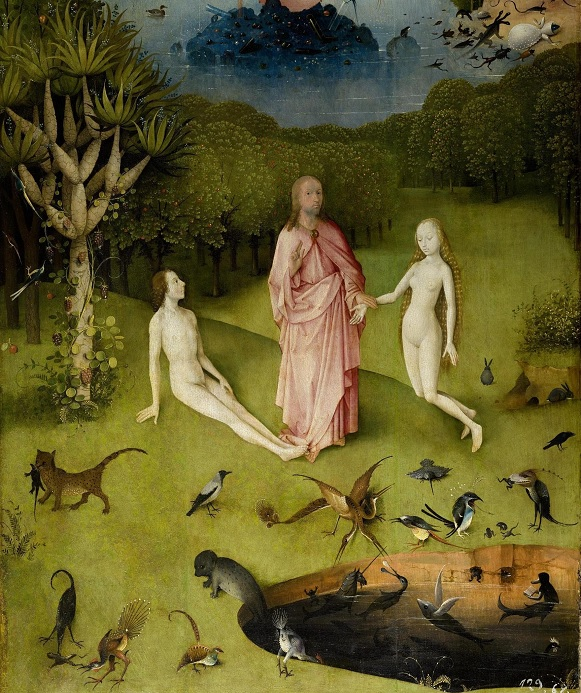
\includegraphics[scale=.3]{a20140926TheEdenicState-img001.jpg}
\caption{Earthly Delights}
\end{wrapfigure}

\paragraph{The Event Horizon}
Trying to understand the Genesis creation story historically and scientifically presents an immediate difficulty. Looking back in time, all we see is death and corruption. Any Edenic or primordial state is beyond that horizon and inaccessible to historical, archaeological, or scientific investigation. Nothing materially incorruptible could have survived until our time.

\paragraph{Psychic Layers}
In any case, it is not the historical events and conditions that counts, but rather their meaning. \textbf{Valentin Tomberg} develops a method of meditation which he attributes to \textbf{Carl Jung}. This involves ``the exploration of psychic layers as the living past of the soul. The entire past lives in the diverse layers of the depths of consciousness." So instead of looking back, we look inward to discover all the states of consciousness involved in the creation of the world and man.

God created the basic elements — light (fire), water, air, earth, and life — all of which are prerequisites for the possibility of manifestation. These elements symbolize energy and the three states of matter. Life signifies interiority, so that the world has an ``inside" as well as an ``outside". It is this interiority that makes such a meditation possible.

We have previously described this method to understand the cause of the Fall in \textit{Doubt and Certainty}\footnote{\url{https://www.meditationsonthetarot.com/doubt-and-certainty}}. With the help of the two Fathers who have described the primordial state in some detail, we offer suggestions to understand that state through the meditation of the psychic layers.

\paragraph{Image and Likeness}
Man was created in the image and likeness of God. These refer to the two poles of being, which is made clear because man is created both from spirit and dust:

\begin{itemize}
\item \textbf{Image of God}: This is man as created, so it is a passive quality. Just as a work of art brings glory to the artist, the image of God in man bears glory to God, not to man himself. This was not lost in the Fall. 
\item \textbf{Likeness to God}: The likeness to God occurs as man grows more god-like, which is called theosis. As an active quality, the likeness requires actualization and manifestation. This was lost in the Fall and its recovery is the goal of reintegration. 
\end{itemize}
Obviously, man as the image of God does not mean that God has a human type of body. Rather it means that man is distinguished by the rational, or intellectual, soul. Note especially that this does not mean that man \emph{has} reason, but rather that he \emph{is} reason. Man's body and lower soul is formed by the intellectual soul.

There is a lower and higher intellectual soul. The lower knows through discursive, logical, and sequential thought, the higher through direct intuition.

\begin{itemize}
\item \textbf{Lower intellect soul}: its function is to perceive the material world, then organize and evaluate these perceptions. 
\item \textbf{Higher intellect soul}: the higher function is to perceive spiritual realities. E.g. other people as spiritual beings, angels, and God 
\end{itemize}
These will be explained in detail in the forthcoming post on knowledge in Man, God, and Angels.

In the primordial state, the intellect works harmoniously with \emph{eros} (or \emph{epithumia}) and \emph{thumos}, the physical center and emotional center, respectively.

Thus man's real existence is interior: ``Although our outer human being is perishing, the inner is renewed day by day." [2 Cor 4:16]

\paragraph{New Age Distortions}
There are two new age distortions of this teaching, one for each pole. The first is the claim that everyone is a ``child of God" by birthright. The actual teaching is that only the baptized, i.e., those on the path to theosis, can be called children of God. The true meaning is that every human is created in the image of God, but that does not bring any glory or credit to that person.

The other is a corruption of the Vedanta idea that ``Atman is Brahman"; For example, people tell me, ``I am God," when I can see perfectly well that they are not. By that, they mean that in their fallen state they are somehow God-like. As we have seen, that is completely false. It is only by the reintegration to the Blessed State through theosis that makes someone ``God-like".

\paragraph{The Blessed State}
Since God is holy, passionless, and sinless, man in the blessed state is likewise holy, passionless, and sinless

\subparagraph{Holy}
The word for ``holy" in Greek and Hebrew means ``set apart", in English, it derives from ``whole". This refers to the Real I which is apart from and transcendent to the world. (``I am in the world but not of it.") The Real I also represents the unity of the being, since it ties all the parts together.

The holy man has no need of any law (with one exception), since a law commands us to do good and avoid evil. In Eden, all creation was good, hence there was no need to know evil.

\subparagraph{Changeable}
God is unalterable, unchangeable, and simple. Man, on the contrary, is alterable, changeable, and composed of parts. Although free from physical privation, there was still the possibility of mental privation. That is the meaning of the tree of good and evil. In other words, there was the possibility of knowing evil, but not the actuality. The Fall made that possibility actual as described in \textit{Doubt and Certainty}\footnote{\url{https://www.meditationsonthetarot.com/doubt-and-certainty}}.

Therefore, man as free was commanded not to eat from the tree lest he die. That was the only law.

\subparagraph{Sinless}
As created, the Will follows the Intellect. In the Primordial State, man was holy and he knew God directly through his intellect. As there were no distractions to the Will, it followed the Intellect faithfully. Hence, man was sinless.

This does not mean that man, such as he is, is sinless; that is the assumption of the modern mind. This usually is expressed that God created us a certain way, so our inclinations and peccadillos are how he wants us to be. Quite the contrary, we are to overcome such inclination and achieve the likeness of God through theosis.

There is a common misunderstanding about free will. The common opinion is that it means we can choose this or that at will. The deeper understanding of free will is that it means that we can never be compelled to choose evil. The practical application of this understanding is an exercise left to the reader.

\subparagraph{Passionless}
Passionless means that man in the primordial state was not subjected nor reactive to forces from below. It does not mean that he was cold and without feelings. After all, the world has an inside that can be felt deeply. Poets, artists, mystics, and even ordinary people have sometimes had this feeling of the world erupt into their consciousness. Although that feeling is quite profound, and even transforming, it is still natural and not the same as the unitive experience of theosis.

So passionless means that the Intellect rules over the passions; in particular, negative emotions cannot arise. Another way to put this is that the ``subtle rules the dense".

St Basil has an interesting interpretation of the command to ``rule" the animals. He allegorizes the animals as representing various emotional states, which must be ``ruled" by the Intellect.

The command to multiply means to increase our own spiritual growth.

\subparagraph{Conditions}
In the primordial state, man was immortal and incorrupt. There was no sin, sorrows, cares, or difficult necessities; there were no labors, no misfortunes, no disease, and no accidents.

These are the conditions that the New Age teachings assume as natural. The New Ager will assert that all is perfect, whole, and complete. Christian Science, in particular, claims to be based on the knowledge of those conditions.

However, those conditions only apply to man in the Primordial State. All affirmations, denials, treatments, visualizations, and so on are ineffective otherwise. A fortiori, all social programs to recreate the Edenic conditions are similarly doomed to failure. The modern mind rejects everything necessary for reintegration. They assume that:

\begin{itemize}
\item Man is not holy, but rather a part of nature. 
\item Man is not ruled by the Intellect, but rather by passions. These must be protected at all costs. Without passion, man is nothing. 
\item Man is not sinful, so whatever he is or does needs to be tolerated and accepted. 
\end{itemize}
Reintegration is based on the opposite of each of those assumptions.



\flrightit{Posted on 2014-09-26 by Cologero }

\begin{center}* * *\end{center}

\begin{footnotesize}\begin{sffamily}



\texttt{Marcel K. on 2014-09-26 at 13:31 said: }

Cologero,

I am a silent reader and since this is my first comment I want to thank you for the great work you've done with this blog and the profound insights you've given to us.

Since it is something I currently struggle to understand, I wanted to ask you if you could expand on the distinction between the state of passionlessness and the absence of feelings (or coldness)? I think you're telling us that it is possible to quench our passions without practicing a form of religious quietism, i.e. the complete suppression of our worldy efforts. Personally however I haven't been able to achieve a deep understanding of this distinction. It seems to me that whenever I think I begin to understand, it immediately slips from my grasp and I revert to a state of not-understanding. 

I've been wondering whether the distinction is blatantly obvious and my inability to comprehend simply a result of faulty thinking on my part, or very subtle with deeper implications than unsubtle distinctions.


\hfill

\texttt{Logres on 2014-09-26 at 22:08 said: }

If man is a microcosm, then the individual becomes just like Nature as we see it: that is, there is a blind, groping manifestation of undulating movement (which we mistakenly call ``real life" and identify our personality with), and then there is what the Catholics would call the ``hidden soul", which is what's left of the image of God in man. Just as the natural world undulates or groans for redemption, but by itself cannot manifest the Logos, so the fallen being is gripped by a fierce passion(s) which smothers up the waters of Life. Whoever wins at ``real life" loses, says Mouravieff, whoever ``loses", wins. The analogy, he states, is almost exact. Isn't this what is meant, the ``last will be first, the first last"? So the emotional (thumos) level of being is the aim of esoteric work, as it is embryonic, the astral foetus, and like embryonic tissue, is easily distorted by the power of the passions' toxins it is exposed to, in that under-developed state. That's why the personality has to ``die" in the dark night of the soul…it seems like cutting yourself off from Life, like an addiction. In reality, it's the way out that is ``deeper in".


\hfill

\texttt{Cologero on 2014-09-27 at 21:22 said: }

Marcel, that is a life's work, not a comment. Passionlessness means that one is not ruled by the lower passions. On the other hand, there are legitimate feelings that motivate our wills or else we'd be machines. I guess there is a subtle difference between the passions ruling or motivating. When the negative emotions are ignored, there is the possibility for higher feelings of joy, peace, etc. to appear. It requires study, e.g., in the Philokalia or Clement of Alexandria. And along with that, a lot of practice in observing the passions and learning not to be reactive.


\hfill

\texttt{Caleb on 2014-09-28 at 16:07 said: }

Marcel, 

It may help in understanding passionless to contemplate Aristotle's `Unmoved Mover.' Consider the relation of the Sun to the other heavenly bodies which orbit it. Its position relative to them remains unmoved, and yet even though it just sits there in the center, its mere presence determines the movement of the other celestial bodies through its gravis. One certainly would not describe the Sun as cold however! 

Passion can be defined as ``that which moves us." The sun, through its immense presence is not moved by the other bodies, which by traditional understanding represent the passions (Venus driving desire, Mars driving anger, the moon driving the subconscious, etc). God likewise is as the sun, the center and source of all things, which move in Him, while He, in His aspect of transcendent unity, remains unmoved, because He is the center. That is the ideal which we aim for as we make our way back to the center.


\hfill


\end{sffamily}\end{footnotesize}

\section{The Primordial State}

\begin{quotex}
The present age must come to terms drastically with the facts as they are, with the absolute opposition that is not only tearing the world asunder politically but has planted a schism in the human heart. We need to find our way back to the original, living spirit which, because of its ambivalence, is also a mediator and uniter of opposites, an idea that preoccupied the alchemists for many centuries. \flright{\textsc{C G Jung}, \emph{Aion}}

\emph{O felix culpa quae talem et tantum meruit habere redemptorem}

“O happy fault that earned for us so great, so glorious a Redeemer.” 

\end{quotex}
Memory of the Primordial State was retained in several traditions. In \emph{Man and his Becoming}, Rene Guenon describes three stages leading to Union: in ascending order, \emph{balya}, \emph{panditya}, and \emph{mauna}.

In Balya, or the Primordial State,

\begin{quotex}
all the powers of the being are concentrated in one point, realizing by their unification an undifferentiated simplicity, comparable to embryonic potentiality. It means the return to the `primordial state'. 

\end{quotex}
In that state, the powers of the being are concentrated in the Self, which is the unifying factor. In the natural state, man is not unified under a unified will. He is uncertain, opinions and desires change from minute to minute, unconscious drives cloud the intellect, knowledge is hard to come by.

Guenon then compares it to the Western analogue:

\begin{quotex}
This is the `Edenic state' of the Judeo-Christian tradition; it explains why Dante placed the Terrestrial Paradise on the summit of the mountain of purgatory, that is to say at the exact point where the being quits the Earth, or the human state, in order to rise to the Heavens, described as the `Kingdom of God'. 

\end{quotex}
The balya stage is childlike because of the analogy to embryonic potentiality. Jesus implies the same idea:

\begin{quotex}
Whoever does not receive the kingdom of God like a child shall not enter it. \flright{\textsc{Luke 18:17}}

\end{quotex}
This is the state enjoyed by Adam and Eve. Nevertheless, it is only preparatory and is far from the state of Union (\emph{mauna}) or the Beatific Vision.

\paragraph{Life in the Edenic Bower}
\begin{quotex}
That spot to which I point is Paradise,

Adam's abode; those lofty shades his bower. \flright{\textsc{John Milton}, \emph{Paradise Lost}}

\end{quotex}
Origins are always a mystery.

\begin{quotex}
In paradise man would have been like an angel in his spirituality of mind, yet with an animal life in his body. \flright{\textsc{Thomas Aquinas}}

\end{quotex}
Adam awoke from his slumber with an enhanced consciousness. He was able to name the plants and animals. That is, he knew them by their natures or essences, not just as material objects. Pythagoras claimed that it was the wisest man who gave names to things.

Adam was formed, not made. To be formed means to be informed by one's essence. The form acts on matter to make it what it is. At that point, Adam was no longer an animal. He had an intellectual soul. He was a person, since he had an individual name, not a species name like the animals he named.

To make is to construct from existing material parts. I can make a mousetrap. I can even make the cheese (although it is much easier to just buy it). But I cannot make a mouse out of existing parts. A mouse can only be conceived, grow, and be informed by mousiness. There is no divine essence for a mousetrap. That is the difference between a natural kind and an artifact.

As he looked about, he saw the animals. There were vegetarians, and the predators of those vegetarians. He saw them give birth, live, hunt, and die. But as a fully conscious and aware being, he was able to avoid danger. He knew the healthiest foods for himself. He knew the healing powers of the various herbs if any problems came up.

He looked for others like him. There were beings who were similar to him in outward appearance, but quite different in their interiority. There was one who grabbed his attention. She was a woman, just like him, “bone of my bones, and flesh of my flesh”. He named her Eve and took her as his wife. They belonged to each other, and no longer with the beings they had derived from. In particular, they had to separate from their parents.

\begin{quotex}
a man shall leave father and mother, and shall cleave to his wife: and they shall be two in one flesh. 

\end{quotex}
Adam and Eve were innocent and unashamed.

\paragraph{Innocence}
\begin{quotex}
Freedom from evil desire is known as innocence. In the state of innocence, man's reason keeps the lower part of his nature, namely his body and its senses, so much in subjection that the latter can never interfere with the free deliberation of the mind, but continues to be wholly subservient to it. Reason can then activate the powers of the will, and, when they are excited, curb and suppress them. The first human beings had a nature that was pure and strong, and they had powerful and healthy bodies, nor were they denied the delights of sense, though these were always kept under control and subjected to the reason. \flright{\textsc{St Thomas Aquinas}, \emph{Summa Theologica} I, q. 98, a. 2}

\end{quotex}
In the primordial state of innocence, there are four transcendental, that is, preternatural, attributes that are missing or depraved in the natural state:

\begin{itemize}
\item Knowledge 
\item Integrity 
\item Impassibility 
\item Immortality 
\end{itemize}
\paragraph{Knowledge}
Theologians commonly refer to three areas of special knowledge possessed by Adam: regarding God and His attributes, the moral law or man's relations to God, and the physical universe both material and spiritual.

In Adam, the knowing functions appropriate to men were perfect. These are

\begin{itemize}
\item \textbf{Sense awareness}: His impressions of the world revealed to the senses were without distortion. 
\item \textbf{Rationality}: The intellectual soul separates Adam from the animals. He is rational and can follow a logical argument. That is quite rare today. 
\item \textbf{Intellection}: He had the higher functions of intuitive knowledge. Unlike rationality, this is a direct, unmediated grasp of an idea. This is the way angels know. 
\end{itemize}
In addition, he had special infused knowledge which follows from those functions.

\begin{itemize}
\item \textbf{Reality}: He had accurate knowledge of the world and of other people. 
\item \textbf{The Moral Law:} He knew the moral law and man's relationship to God. This means he also had complete self-knowledge and internal psychological processes. 
\item \textbf{Transcendence}: He had knowledge of God and his attributes. 
\end{itemize}
Adam knew Eve perfectly,

\begin{enumerate}
\item First as the image he had of her in his soul 
\item Then as a person in the flesh 
\end{enumerate}
There was no conflict between them.

\paragraph{Integrity}
Integrity means wholeness, so that Adam was unified in body, soul, and spirit. His Self was master and his desires and emotions were subjected to the dictates of reason and free will.

Adam did not experience any division or discord within himself. This was reflected, also, to his outer life. Integrity is the conformance of the interior man to the exterior man in his life, speech, and actions.

\paragraph{Impassibility}
Impassibility is freedom from suffering. In particular, one is free from negative emotions, such as hate, fear, rage, jealousy, depression, anxiety, worry, uncertainty, melancholy, annoyance, boredom, lack of self-confidence, and the like. That is anything that adversely affects one's quality of life.

Yet this is not a stoical state. In the Primordial state there are positive emotions including love, joy, satisfaction, contentment, serenity, awe. Moreover, even the negative emotions may have their place as long as they are intelligent. There is a healthy fear that protects us from danger. Anger can motivate positive actions to fix problems.

The preceding emotions are experienced in the lower emotional centre, or thumos. Above that there is a higher emotional centre, often called the Heart. Whereas the lower centre is oriented to the world, the higher centre is oriented upwards. Emotions are of a different class and more intense, such as bliss, gratitude, and other emotions that have an analogue in the lower centre.

In the lower centre, suffering is not willed. However, in the higher centre, one can take on suffering voluntarily. Fear of God, or regret for one's sins, are emotions that sound negative, but are not, because they are willed.

\paragraph{Immortality}
The Body was not a burden in the primordial state, since it was responsive to Adam's will. It was not affected by disordered emotions like anxiety, fear, boredom, excessive desire, etc., which adversely affect the systemic functions of the organism.

Adam able to avoid all dangers. Since he was fully aware of himself and his surroundings, he was able to avoid external dangers like accidents, wild animals, fire, and so on. Accidents result from

\begin{itemize}
\item momentary lapses of concentration 
\item ignorance of cause and effect 
\end{itemize}
Internal dangers like sickness, poison, ageing, and the like were also thwarted. The I not only had mastery over the emotions and desires, he also had mastery over the body. As we can see from the examples of yogis, fakirs, saints, and even contemporary magicians and endurance performers, there is more mastery over the body than we admit. Saints would be singing even while being tortured to death.

In the Primordial State, there is concentration and meditation. \textbf{Valentin Tomberg} describes the effects of deep meditation in \emph{Inner Development}.

\begin{quotex}
What is striven for, and achieved, by means of meditation is a new relationship between spirit, soul, and body. The spirit approaches the human being, it inclines downward; the soul becomes larger; and the body becomes ensouled. This is the body's inner purification. It becomes pure when everything bound up with its life is permeated by the heart. Nothing in life is ugly if the heart is present. Everything cynical that is said about the life of the body occurs through the fact that those who say such things lack the experience of the soul permeating the body. When the soul permeates the body, the body is raised to the dignity of the soul. Through meditation, a harmony arises between body, soul, and spirit—a harmony that is attained when the spirit inclines downward, the soul expands, and the body is raised to the dignity of soul. 

\end{quotex}
\paragraph{The End of the Beginning}
As pleasant as life in the Edenic Bower must have been, without suffering, anxiety, or unfulfilled desire, it had a terminus. Like Limbo or the Buddhist heaven, there was no possibility for ultimate deliverance of the Beatific Vision.

Although he was virtually immortal, Adam was obviously not actually immortal. Evil tempted him. He tried to extend mastery over himself to mastery over the entire world, which in effect is to take over the role of his creator. The delicate balance between his Ego and his Self descended into the Ego.

Only a saviour who combined both natures could, not only restore the balance, but lead to the Beatific Vision.



\flrightit{Posted on 2020-09-06 by Cologero }

\section{The Fall from the Primordial State}

\begin{wrapfigure}{rt}{.3\textwidth}
 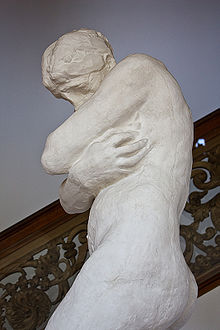
\includegraphics[scale=1.5]{a20110111TheFallfromthePrimordialState-img001.jpg}
\end{wrapfigure}

Let us be clear. The \textbf{Primordial State} is not a ``state of nature" as in Rousseau, but rather of supernature. But if in the Primordial State man lives in harmony with nature and the divine, with a direct awareness of God in his psyche as his life force, and with bonds of loyalty to his family and nation, then what would account for a change in consciousness? Table~\ref{tab:FallPrimordialState1} shows the effects of the Fall in the \emph{Genesis} account, and the corresponding condition that was affected.

\begin{table}[h]
\centering\small
\begin{tabular}{cc}\toprule
\textbf{Effect of Fall} &
\textbf{Consciousness before fall}\\\toprule
Toil &
Concentration without effort\\\midrule
Suffering &
Natural joy\\\midrule
Death &
Transformation\\\bottomrule
\end{tabular}
\caption{The effect of the Fall according to Genesis book.}
\label{tab:FallPrimordialState1}
\end{table}

\paragraph{Effects of the Fall}
The point to keep in mind is that the Fall is an event in consciousness; it is necessary to meditate on the symbols of the fall, and the description of the states, to fully understand.

\begin{description}
\item[Toil ]

Everyone has had the experience of being totally absorbed in an activity, to the extent that time seems to stand still. One feels energized and does not tire. Similarly, composers and poets have often described moments of inspiration, and the poem or symphony seems to write itself. This state of ``concentration without effort" is comparable to the Taoist ideal of \emph{wei-wu-wei}, or doing-nondoing. After the fall, concentration becomes difficult and labored; one becomes restless and bored; activities begin to feel like toil. 

\item[Suffering ]

Man lived in a state of natural joy. The sensory experience of the natural world was vivid and pleasurable; it did not require a special trip to a resort. Man was in communication with the gods and angels, was aware of the presence of his ancestors. He lived in peace with his nation and leaders without private concerns. This was replaced with feelings of resentment and ambition. This led to frustration, anxiety, shame, guilt, and fear. Man became alienated from nature, from the divine, from his nation, and leaders. 

\item[Death ]

Death was understood as a natural process and it represented a transformation. A man was prepared for his death by understanding the post-mortem states of being. He was aware of his ancestors and felt his immortality in his descendants. After the fall, man lost direct awareness of the divine, of his ancestors, of post-mortem states, of his own true Self. Death became something to fear, something that signified destruction rather than transformation. 

\end{description}
\paragraph{Perversion of Soul Life}
The psyche, or soul, which had been a pure reflector of both nature and the divine, becomes obsessed with the effects of the fall. The consequence is that the formerly direct intuitive awareness of nature, the divine, and nation becomes occluded. The true Self is decentered and a false self is established. \textbf{Julian Jaynes} describes the characteristics of this state. [See Note.]

\begin{description}
\item[Spatialization ]

A mind-space model of consciousness is invented. 

\item[Excerption ]

Consciousness is focused on just a part of experience. The vividness of the Primordial State is lost. 

\item[Analog I ]

A model of one's self is created in consciousness. This acts like a little god in one's own consciousness, with its own plans. 

\item[Objectification ]

Beyond the ``I" as subject, the self becomes an object in consciousness 

\item[Narratization ]

There is a running narrative consisting of a web of thoughts. This narration forms our very identity. Thus, it becomes very difficult to alter since that would be felt as a threat to oneself. 

\item[Assimilation ]

Experiences are forced to fit into pre-conceived or remembered patterns. This makes it very difficult to understand, or even hear, new ideas. 

\end{description}
\paragraph{Initiation}
Initiation means conscious experience of the beginning, that is, of the Primordial State. The various traditions have arisen in order to lead back to the Primordial State.


\hfill

NOTE: Julian Jaynes, in his remarkable book, \emph{The Origin of Consciousness in the Breakdown of the Bicameral Mind}, brings historical evidence to a change in consciousness similar to what has been described. Unfortunately, it is sui generis, and due to some faulty assumption, the author was never able to develop his insights further. In particular, he regards the Primordial State as a state of unconsciousness and the fallen mind as the beginning of consciousness. Tradition sees it just the opposite.



\flrightit{Posted on 2011-01-11 by Cologero }

\begin{center}* * *\end{center}

\begin{footnotesize}\begin{sffamily}



\texttt{KarlH on 2011-01-11 at 11:20 said: }

I haven't read Jaynes' book, but there are a few things worth noting:

The Judaic tradition didn't originally consider the ``Fall" to be a Fall. In fact, those who study early Judaism are often startled to find that the story was rather an expression of the idea that man had, in a sense by eating from the tree of the knowledge of good and evil, grown up. With this comes certain responsibilities and all the things that make life tough, but it is all according to God's plan and even these frustrations make life worth living. In fact, suffering makes it all the more meaningful.

The interpretation of Genesis as a ``Fall" comes from Zoroastrian influences. Rather than the serpent being an angel of temptation who really stands alongside God, the serpent is instead a force of Evil and the act of eating from the tree is seen as a transgression against the cosmic order.

There is another idea worth mentioning and perhaps you've considered the same. Even in Origen who adopted the vogue interpretation of Genesis as a Fall, Origen proposes (and this idea was echoed in a few of the early Fathers) that although the Fall has given us a number of woes and misfortunes, it may, in the end, be a Good. He considers that it is all God's plan and that the Fall was actually a good thing, perhaps BECAUSE of the terrible things it unleashed. Even if ``Tradition" describes a Primordial State of non-differentiation that we're trying to return to, it doesn't necessarily follow that things are getting worse. Sure, things are getting worse in a sense, but in this confusion, division of languages and lack of unity (see: Tower of Babel), man has actually learned the process of learning. Man has actually known pain and suffering and there are now heroes and saints and philosophers. The saint needs the sinner and so on.


\hfill

\texttt{KarlH on 2011-01-11 at 11:43 said: }

Note: obviously, in the texts, there is the idea that man has ``lost" something. But what has he lost? His childhood, of course. He can now pursue knowledge and exercise free will in pursuit of the Good in a multivarious fashion. He is separated from his Father, but he can still follow him. He is now hampered by a very finite life and a number of bodily ills, but he can turn even this suffering to the glory of God. In this, all his corporeality, all his sickness and all his hardship can be transformed without really being ``altered" in the objective sense. Bodily nature and all its woes is transformed because it focuses on what is honest, pure and true and even the /apparent/ negation of such (corporeality, sickness, and hardship) becomes a positive affirmation of the Good. We must all remember that it is really impossible to escape from God: nothing escapes Him and nothing is apart from Him, even nothingness.


\hfill

\texttt{KarlH on 2011-01-11 at 12:00 said: }

On the other hand, if you're looking at capital ``T" traditon then you'll have to ignore a large number of data and instead misappropriate texts to suit your own purposes as there are no other canonical texts in the Jewish tradition to make the point you want to make which was introduced to the Western Tradition by Plato (or whoever he got his ideas from—I imagine that the Timaeus was strongly influenced by popular religion). You don't really have any other alternatives if you're sticking with the Roman Tradition. It is founded upon ignoring the context of a number of Jewish traditions and interpreting texts to suit whatever Greek-influenced idea needed to be introduced.


\hfill

\texttt{Will on 2011-01-11 at 12:35 said: }

KarlH, I think it's inaccurate to describe the Primordial State as one of ``non-differentiation." Rather, it is non-dualistic. The difference is that non-differentiated would be a kind of monism in which all is one and everything is equal to everything else. Non-dualism, in contrast, says that God, or the Absolute, and the creation / emanation are not one and the same, but are not wholly separate either. In this view, differentiation is a natural complement to emanation. As in the Tao Te Ching, from one to two to three to the ten thousand things.

The non-dualist view retains the importance of qualitative distinctions on the relative plane, whereas the monist, non-differentiated view seems to be prominent among new agers, and forms the metaphysical backdrop to their all-embracing naivete. ``All is one, all is God, hooray!" while the world crumbles around them. There's a sense in which that's true, of course, since as you say ``nothing escapes Him and nothing is apart from Him." But it seems to me this view informs a delusional escapism more often than a genuine realization.

Also, it seems to me that your second comment reduces the Genesis myth to a mere psychoanalytic metaphor. Yes, childhood does have a certain wholeness and ease compared to adulthood, and maybe that is somehow related to a greater connection to the Primordial State, but I think here again this kind of view often gives rise to an error. If the Primordial State is childhood, then the best example of returning to it would probably be something like Kevin Spacey's character in American Beauty, who forsakes his job and family life to live like a teenager again.

There's a sense in which that kind of life is indeed better than the typical, slavish bourgeois life of middle America. For one, it has a sense of awe and wonder about the world which most people lose as they grow older, through the Perversion of Soul Life which the post describes. But it seems to me that a true return to, or realization of, the Primordial State transcends this childhood-adulthood dichotomy.


\hfill

\texttt{Will on 2011-01-11 at 13:28 said: }

Addendum: The last paragraph of my comment should read ``a process somewhat analogous to the Perversion of Soul Life which the post describes." As I originally wrote it, I'm guilty of the very reductionism I was criticizing. Hate it when that happens.


\hfill

\texttt{KarlH on 2011-01-11 at 14:00 said: }

I realize the first point you've made. Non-differentiation wasn't perhaps the best term and I noticed that after the comments I posted but didn't want to clutter this commentbox more than I did already. For reasons beyond my control, it's been difficult for me to order my thoughts coherently for the past few weeks. I don't say this to elicit sympathy but to acknowledge that I currently struggle to make myself understood with a hampered intellect but I'll do the best I can and if I seem a bit unclear/something stands out as a glaring error, it may (or may not) be due to this.

In short, I think you've misunderstood the main point I made: I was pointing out that the interpretation of the Fall doesn't exist outside of later rewrites by those who wanted to write-in Greek-influenced ideas into the Old Testament stories and allegories so perhaps it's a bit dishonest to claim that we're uncovering some old doctrine/piece of Tradition when we talk about things like the ``Fall" and attach it to Genesis. On the other hand, as the Christian tradition really has no other alternative to express the belief in this Primordial State, perhaps it's okay to use Genesis for this purpose so long as we're honest about our dishonesty.

On the other hand…I did choose the word non-differentiation for certain purposes but perhaps it doesn't make sense in the context I used it. I meant non-differentiation such as the non-differentiation of the sexes mentioned in Plato's account of creation/St. Gregory's. There is, apparently, a lot more differentiation between the Primordial State and now. A unity of opposites must therefore be our goal. But it is not so much a goal as an acknowledgment that can be lived and expressed and upon which we can ground ourselves.

I think you understood my second comment by misunderstanding it. I'll expound: I think it is worth considering that it's okay we fell away from the state we were in before (whether or not this state is identical to what we consider to be the ``Primordial State" and this falling-away gives the opportunity for synthesis between the ``fallen" qualities that emerged (a conception of individuality outside of community, sickness, etc.) and the original state. And now I feel like I'm just quoting Steiner…

I think I am really critiquing the lack of tradition in ``traditionalism." The ancient Jews had little conception of a ``Primordial State" with the extent of powers attributed to it in this article. And even if they did, they didn't see being thrown out of the garden as an evil. How can we reconcile this knowledge with this article? If we're actually striving for honesty and truth, we'll acknowledge that our conceptions of the Genesis account are based upon non-Judaic sources and perhaps aren't true to original intentions. This doesn't mean interpretations can be developed, but sooner or later we have to acknowledge that our use of texts is similar to inkblot projections.

I don't think there is anything New-Ageish about my beliefs and I've fought against the non-historical tendencies of such, whether they are modern feel-good liberals of Suburbia or a few revered philosophers who practiced Platonism at the expense of the kindness they could have shown to the souls in slavery and bondage around them. I believe strongly in the existence of qualities (beyond a vague pragmatism for achieving Enlightenment) and the importance of living a life that engages with existence in its totality and doesn't seek to escape it with vague syllogisms or ideological idols. This has made life very difficult yet very meaningful for me. I've already been interrupted 17 times writing this comment, and this is due to the fact that I'm not really ready to give up on the world and seek some sort of non-existent gnosis—rather, my search for ``Enlightenment" at the moment consists of staying home and helping my mom out/being a good role model for my younger siblings.

Part of my commitment to not-committing myself to idols is that I think we should exercise a certain skepticism when it comes to unraveling the philosophia perennis. Or, better put, we should be skeptical about the bases upon which our evidence lies.


\hfill

\texttt{KarlH on 2011-01-11 at 14:10 said: }

Best summary I can give of my primary objections to certain heresies I've found in Christianity/the Roman Tradition:

1. A number of early Jews saw the garden narrative as a narrative of mankind's infancy. By leaving the garden, he left childhood ignorance behind but has the ability to retain ideality and unite it with a world that legitimately suffers and is filled with toil and difficult things.

2. Our conceptions of Fall/any sort of doctrine grounded upon the philosophia perennis must realize that our monotholic interpretations of things are reductionist and based upon what we want to find in the texts, not being entirely honest to intentions of original authorship/older interpretations of religious communities. And maybe if we're honest about being dishonest to original intentions and realizing that we're projecting essential elements of the philosophia perennis to texts that may or may not support it, it's okay because those in the Roman Tradition are tied to Catholicism and a relatively closed canon wherein essential doctrines and dogmas must be based upon Scripture.


\hfill

\texttt{GF on 2011-01-11 at 14:10 said: }

KarlH,

You are looking at this from a limited perspective, which leads you to think you see something Cologero doesn't. The fall and the intervening stages are necessary and good, but return to the Adamic (primordial) state is undeniably the goal and essence of Christianity. This has nothing to do with esoterism or Roman misappropriation – just basic Christianity.


\hfill

\texttt{KarlH on 2011-01-11 at 14:33 said: }

GF,

I recognize this—returning to the Adamic state is central to Islam and Christianity. But it is less so to Judaism for certain reasons, though the ideal of a self-realized/Enlightened person in any of the three traditions would look the same throughout. My last comment makes my points a bit clearer.


\hfill

\texttt{KarlH on 2011-01-11 at 14:59 said: }

I might also add that I doubt Cologero disagree on anything of importance unless he's fallen into the heresy that the Fall and diminishment of man's powers and ability to influence things is an evil. He didn't say whether the Fall of man is or is not an evil, so I was making the point that it's not (or maybe it is—I appreciate that he focuses on the effects primarily).

The issue is that in using the word ``Fall," we are conceiving man as actually moving away from the Absolute. Yet the diminishment of mankind's powers really says nothing about his objective relation to the Absolute as we never really escape it. We must strive for perfect clarity when it comes to talking about a ``Fall" because of the number of heresies that have stemmed from focusing on it and have led to atrocious conceptions such as Total Depravity, notions upon which the Americas and Western Europe are founded.


\hfill

\texttt{GF on 2011-01-11 at 16:07 said: }

I don't believe he ascribes a primarily moral significance to the Fall; here, in fact, he's asserting the Hermetic significance of a division of consciousness. So the issue is wholly subjective. That was clear to me; all the same your clarifications are welcome. 

You might be interested in d'Olivet's The Hebraic Tongue Restored, which includes a radical retranslation of the first ten chapters of Genesis based on the Sefer Torah. It can be downloaded from the Internet Archive.


\hfill

\texttt{GF on 2011-01-11 at 16:14 said: }

Your comments about early Jewish religion are appreciated. I do not know much about it, nor am I particularly interested, so I guess that falls under `honest dishonesty'. Still, you might be surprised by d'Olivet; the Egyptian or Hermetic connection between Mosaic and Platonic metaphysics is strongly attested. Even secular commentators have noticed this, some going as far as claiming that `Moses' plagiarized from Plato or vice versa.


\hfill

\texttt{Cologero on 2011-01-11 at 19:48 said: }

Yes. Not a moral significance, nor is it intended to refer to just the Hebrew scripture. To the contrary, we are discussing the cosmic cycles which is generally interpreted as a decline in all traditions. We can add the following points:

1) The Talmud is not necessarily the authoritative interpretation of Genesis. The religion of the Talmud differs in substantive ways from the Hebrew Scriptures.

2) If the Edenic myth is simply about some pedestrian notion as the growth from childhood to adulthood, then why is it necessary to portray it in mythological symbolism?

3) And this is the most important, and it was mentioned in the post. The matter is ultimately not settled by debate, but by the meditative experience of initiates (i.e., those properly qualified) which reveal the inner structure of consciousness as described in the post.


\hfill

\texttt{kadambari on 2011-01-13 at 10:06 said: }

``I don't really think those in the movement have successfully realized how enormous the criticisms Buddhism gave to speculative metaphysics in their Golden Age, for instance."

One of the biggest mistakes is to assume that Buddha was anti-caste and a reformer in this sense. The one who reads Buddhism carefully realizes it differs very little from Hinduism, even metaphysically, only in that gnosis is not restricted to people by birth, but this in no way makes Buddha a crusader against caste, when Buddhism was most powerful and creative when Brahmins became Buddhists and a steady stream of people from the aristocracy were constantly contributing to it.

``Not so much emphasis on actually helping people and the acknowledgment that the caste system and feudal system kind of sucked in some areas because they ignored the potential genius lying among the lower castes."

Again Buddhism was not anti-caste, but gave an outlet for those that

found it restrictive, all this did was in fact to make tradition stronger, by helping to reaffirm the essentials in the old religion which was getting corrupted by too much emphasis on externalities…


\hfill

\texttt{kadambari on 2011-01-13 at 10:22 said: }

Karl H,

Rather one can say Buddhism lead to increase in literacy amongst the masses in India, but did so without altering the traditional structure of society itself in any way, which is why in India there was more spead of literacy than in Persia where religion remained very much an affair of the aristocracy (Dastoors-Persian priests), and literacy as well…


\hfill


\end{sffamily}\end{footnotesize}


\chapter{States of being. The Divine Journey}
\section{Divine Journey Summary}

In \emph{Man and his Becoming}, \textbf{Rene Guenon} outlines a path to liberation. If you start at the beginning and work through it diligently with understanding, you might attain the Supreme Identity. Just as a master mechanic understands the workings of an automobile, the student must have a complete understanding of the inner workings of the human being. These are the main topics in the process, as illustrated in \emph{Man and his Becoming}.

\begin{enumerate}
\item The distinction between the true Self (Atman) and the Ego 
\item God (Brahman) resides in the human heart 
\item The process of manifestation and the play of the three fundamental forces 
\item The origin of thought, mind, the senses, and external organs 
\item The different states of the human being 
\item The five sheaths of the human being 
\item The celestial journey through the various spheres 
\item Union, which is the realization of the identity of the Atman and Brahman 
\end{enumerate}
\paragraph{Postmortem States}
These are the possible outcomes of man's postmortem states.

\begin{description}
\item{\bfseries Longevity} Indefinite prolongation of human individuality in the subtle state.
\item{\bfseries Path of the Ancestors (pitriyana)} After the resorption of human individuality, the being will pass into other states of individual manifestation.
\item{\bfseries Passive Liberation of path of the mystics} Jivatman unites with subtle body until the end of the world. It then unites with Brahman passively, without full realization.
\item{\bfseries Delayed liberation} Jivatman unites with subtle body. Liberation will be obtained, at the end of the cycle, by means of intermediate stages [conditioned postmortem states], and not in a direct and immediate way.
\item{\bfseries Liberated at death} Jivatman does not unite with subtle body, nor pass through other states, but is liberated at death.
\item{\bfseries Jivanmukta} Liberated in life.
\end{description}

\paragraph{Transhuman states}
Guenon describes multiple transhuman states on the path of the Divine Journey. This journey can be made during human life or possibly after. In the Vedic version described by Guenon, each stage may be associated with a god or deva. Unless you were born and raised in India, gods like Agni, Varuna, or Indra elicit no visceral reaction. At best, you can gain an intellectual understanding of what the various gods represent.

However, as Guenon points out, Dante's description is virtually the same. Do not be deceived by the lack of exact correspondences, which should not be expected in symbolic representations. For example, Dante encounters various personages instead of gods at the various spheres. The point is to understand the state of consciousness described. Guenon also points out that the angels represent higher stages of consciousness. For many living in the West, this may be a better path.

\paragraph{Ideal type}
In the Vedanta, the Yogi represents the ideal type. Since our goal is the restoration of Tradition in the West, a different model may be appropriate.

Our path is that of the \textbf{spiritual knight}, who is active in the world. This provides the opportunity to manifest all the possibilities of the Self. King David is one such model: he was a warrior and a poet (Psalms). He lived and loved. Work and love are what matters. What tasks are you called to do? Do you have a love, whether real or aspirational?

\paragraph{Individual Path}
Ultimately, we make the journey alone just as did the Knights of the Round Table, not to mention Don Quixote. There is no operating manual for the Divine Journey, since the specific path depends so much on the capabilities and possibilities of the individual. Oftentimes you don't even know if and when you are on the path. After some consideration, I decided that it is appropriate to use personal experiences to demonstrate this.

So I am doing an experiment using Bergson's and Tomberg's understanding of memory. The goal is not merely reminiscence, but the bringing of the past into the present. That will show the memory in a new light, with the highest being moral memory. The exercise of bringing the past into the present can be fruitful. Only then can you recognize the path you have been on.


\textit{From meeting notes of 12 XII 2022}

\flrightit{Posted on 2022-12-14 by Cologero}

\section{Multiple States in Christianity}

Philippe Guiberteau, a Catholic writer, was preparing an annotated translation (into French) of Dante's \emph{Banquet}. Although M. Guiberteau had been reading Rene Guenon for 25 years, he was still unconvinced about the applicability of the notion of the multiple states of the being to Catholic theology. He was then put in touch with Michel Valsan. There we have the rather odd situation of a Muslim explaining Catholic theology to Dante's translator.

In three letters to Philippe Guiberteau, Michel Valsan demonstrates that Christianity also has a doctrine of the universal Self and multiple states. He shows that the metaphysical doctrine of multiple states, which considers man in his totality, that is to say as a being mainly “divine”, “angelic” and “human”, is present in Christianity. Its developments are illustrated in three parts:

\begin{enumerate}
\item Theology of Saint Thomas Aquinas 
\item The spirituality represented by John of Ruysbroeck 
\item Catholic esoterism, as expressed by Dante 
\end{enumerate}
But before completing the introduction to Valsan's letters, I shall summarize the states of being as explained by \textbf{Adi Shankara} in \emph{Tattva Bodhah}. It will be a refresher to some and to others it may be new. In either case, Valsan will include a chart the encompasses these states and their correspondence to Christian esoteric teaching.

\paragraph{Three Bodies and Five sheaths}
\begin{enumerate}
\item Gross body: Perceived through the senses. 

\begin{itemize}
\item Annamaya-kosha: Physical body. Nourished by food. 
\end{itemize}
\item Subtle body: Known directly, not through senses. E.g., hunger, anger 

\begin{itemize}
\item Pranamaya-kosha: vital or vegetative soul. Nourished by air 
\item Manomaya-kosha: animal soul. Seat of emotions 
\item Vijnanamaya-kosha: Intellectual soul. The doer. Nourished by impressions. 
\end{itemize}
\item Causal body: All inherent tendencies which are the cause of the other two bodies 

\begin{itemize}
\item Anandamaya-kosha: Person in unmanifest condition. 
\end{itemize}
\end{enumerate}
Plants have a vital soul only, animals, a vital and emotional soul, and human beings possess all three sheaths of the subtle body.

\paragraph{Three States of consciousness}
These correspond to the three bodies listed above.

\begin{enumerate}
\item Waking state: experience of the gross world through the senses 
\item Dream state: experience of our individual dream world 
\item Deep sleep state: the absence of objects, emotions, and thoughts 
\end{enumerate}
\paragraph{The Universal Self}
The Universal Self, or Atman, is the final stage of Union well known in Catholic spirituality. Valsan quotes Saint Bernard of Clairvaux in \emph{De Consideration}:

\begin{quotex}
What then is God? That without Whom there is nothing. It is as impossible that anything be without Him as He Himself is without Him. He is to Himself as He is to everything and, therefore, in a certain way, He alone is, who is the very Being both of Himself and of everything. 

\end{quotex}
This does not annihilate the person, because only \emph{in a certain way} is God all Being. This is identical to the Vedantic doctrine of the Supreme Self. The scholastic philosophers can be read on two levels:

\begin{itemize}
\item The ontological level, which stops at Being 
\item The trans-ontic level, which goes beyond Being (Gilson) 
\end{itemize}
\paragraph{Knowledge and Being}
Aristotle and the scholastics taught the identity of knowledge and being. In the former's words, “a being is all that he knows.” Guenon indicates that is precisely what is meant by metaphysical realization. Since scholastic doctrine was close to being a true metaphysics, and there had to have been more to it than just the religious and exoteric aspects.

Valsan turns to the Church Fathers to show that the Way of Knowledge (i.e., Gnosis) was always part of tradition. Then he demonstrates that Dante and the Fedeli d'Amore were perfectly orthodox in their teaching. So with two of the objections out of the way, Valsan continues.

\paragraph{The Multiple States}
Valsan then launches into the notion of the multiple states of the being. Since most readers will be familiar with Dante and Thomas Aquinas, it is better to let Valsan speak for himself. Although it is clear that Dante understands the multiple states, Valsan has to spend some time on Thomas' understanding of the Active Intellect.

Less known, perhaps, are Nicolas de Cusa and John of Ruysbroeck. Nicolas is mentioned in passing. We can point out, however, that he understood the distinction between the indefinite and the Infinite, not unlike Rene Guenon. No number of steps can reach the Infinite, which is beyond all manifestation.

John of Ruysbroeck has been a personal favorite as we have written about him often, as can be found in this link.

Valsan goes into detail to show that Ruysbroeck's understanding is entirely compatible with the Vedantic teaching of the multiple states.

\paragraph{Mythical Creatures}
An intriguing side trip involves Valsan's understanding of so-called “mythical” creatures and how they can be understood with the idea of multiple states.

Daimons, Genies, and Jinns are situated between the angels and humans. In other words, they have a causal body and a complete subtle body just as humans do. However, they lack a gross (or physical) body.

Centaurs, Sirens, and the like, are in a degree of existence between man and animals, so they share the subtle body with both men and animals. Therefore, they would have an intellectual soul similar to man's but lacking in some regard.

{The complete text of Valsan's letters in English can be found here: \url{https://www.gornahoor.net/library/Doctrine_Multiple_States_Being_Christianity.pdf}

\flrightit{Posted on 2021-02-14 by Cologero }

\begin{center}* * *\end{center}

\begin{footnotesize}\begin{sffamily}



\texttt{Duncan on 2021-02-14 at 09:46 said: }

Thank you for this timely post.


\hfill

\texttt{MICHAEL on 2021-02-15 at 06:31 said: }

How is this different or distinct from Steiner's classification of the physical body, etheric body and astral body and their sheaths… ?


\hfill

\texttt{Cologero on 2021-02-15 at 09:04 said: }

If it is just a theory, then the coincidence would be remarkable.

But if the different states of being are observable facts, then we should expect some similitude in the descriptions.


\hfill

\texttt{MICHAEL on 2021-02-15 at 09:51 said: }

Yes, agreed… I don't believe it's a coincidence. Same with Daimons, Jinns, Centaurs and Sirens which reflect the same intermediate stages of being like salamanders, gnomes, sylphs and undines? How unique is Steiner when he links up these intermediate stages in us and the creatures of the world to the interweaving creative actions of the various levels of the spiritual hierarchies?


\hfill

\texttt{Logres on 2021-02-15 at 19:14 said: }

It is a fantastically dense letter, with loads of important references, particularly drawing together undeservedly obscure quotes from non-obscure theological writers. As for the last bit, Iamblichus taught that if we are good stewards of our efforts, we release our daemon, and we obtain a demigod to guide us. There are three divisions of demigods, leading upwards. From history: “An equation for me has no meaning, unless it represents a thought of God.”-and he wasn't kidding. Like ancient Indian mathematicians, Ramanujan only noted the results and summaries of his works; no proof was worked out for the formulae he came up with. He straightaway credited his work to the divine providence of Mahalakshmi of Namakkal, a family goddess whom he looked to for inspiration. The mathematician said that he dreamed of the Goddess' male consort Narasimha, who is denoted by droplets of blood, after which, scrolls of complex mathematical work unfolded in front of his eyes.” \url{https://www.indiatoday.in/education-today/gk-current-affairs/story/srinivasa-ramanujan-life-story-973662-2017-04-26}

There is also the legend of the Little Red Man of the Tuileries \& his attachment to France:

\url{https://esoterx.com/2014/08/07/the-little-red-man-of-the-tuileries-a-prophetic-parisian-imp/}

As possible examples of the latter mentioned stuff.


\end{sffamily}\end{footnotesize}

\section{Astral Symbolism}

\begin{wrapfigure}{rt}{.3\textwidth}
 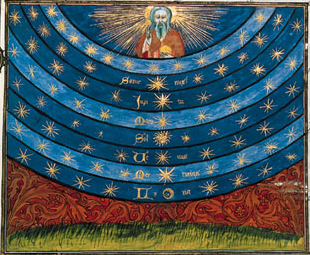
\includegraphics[scale=1.5]{a20220215AstralSymbolism-img001.jpg} 
\end{wrapfigure}

In \emph{Man and his Becoming}, \textbf{Rene Guenon} explains:

\begin{quotex}
Natural phenomena in general, and especially astronomical phenomena, are never looked upon by the traditional doctrines other than as a simple means of expression, whereby they symbolize truths of a higher order.

\end{quotex}
This is true because there is a correspondence between the different degrees. Principles therefore find expression in the human states, as he writes:

\begin{quotex}
If [natural phenomena] symbolize such truths [of a higher order], it is because their laws are fundamentally nothing but the expression of these very truths in a particular domain, a sort of translation of the corresponding principles, naturally adapted to the special conditions of the corporeal and human state.

\end{quotex}
Certainly, this applies a fortiori to astronomical symbolism:

\begin{quotex}
It must be clearly understood, that when mention is made of the Spheres of the Sun and of the Moon, it is never the sun and the moon as visible stars, belonging purely to the corporeal realm, that are referred to, but rather the universal principles which these stars represent after their own fashion in the sensible world … Indeed the different Worlds, planetary Spheres and elementary Realms which are symbolically described as so many regions (only symbolically however, since the being who journeys through them is no longer subject to space), \textbf{are in reality just different states}.

\end{quotex}
Furthermore, as Guenon notes, the same logic applies in the West to the doctrines of Heaven, Hell, and Purgatory. They likewise represent states, not places. Here we have the hermeneutic key to understand Dante's journey. He starts in Hell (the human state), spends time in Purgatory (states of self-purification), and rises to Heaven, passing through all the planetary states.

The same planetary symbolism is also used to represent the chakras. The same understanding applies: the chakras are not physical organs, but represent inner states of the being. Moreover, this understanding is not optional Guenon emphasizes, in regard to these points:

\begin{quotex}
It is absolutely essential for the understanding of these matters.

\end{quotex}
Otherwise, you become like one of:

\begin{quotex}
those who are incapable of understanding anything but the most grossly literal meaning; such people will never realize the workings of a symbol, because their conceptions are irremediably limited to existence on this earth and to the corporeal world, within which, by the most naive of illusions, they wish to imprison the whole of reality.

\end{quotex}
\paragraph{The Literal Meaning}
The symbolic meaning does not debt or replace the literal or historical meaning; rather, the historical event is a consequence of the symbolic or higher meaning. In \emph{The Symbolism of the Cross}, Guenon explains:

\begin{quotex}
The fact is that people too often tend to think that if a symbolical meaning is admitted, the literal or historical sense must be rejected; such a view can only result from unawareness of the \textbf{Law of Correspondence} which is the very foundation of all symbolism. By virtue of this law, each thing, proceeding as it does from a metaphysical principle from which it derives all its reality, translates or expresses that principle in its own fashion and in accordance with its own order of existence, so that from one order to another all things are linked together and correspond in such a way as to contribute to the universal and total harmony, which, in the multiplicity of manifestation, can be likened to a reflection of the principia! unity itself. 

\end{quotex}
To summarize:

\begin{quotex}
The laws of a lower domain can always be taken to symbolize realities of a higher order, wherein resides their own profoundest cause; which is at once their principle and their end. 

\end{quotex}

\hfill

\flrightit{Posted on 2022-02-15 by Cologero }

\begin{center}* * *\end{center}

\begin{footnotesize}\begin{sffamily}



\texttt{TSP on 2022-05-26 at 12:04 said: }

I read something in Guenon's “The Spiritist Fallacy” that has given me serious pause. He denies the astral form and in this he goes against not only Valentin Tomberg, Franz Bardon, the UR Group (see the essay on the “diaphanous body” in “Introduction to Magic Volume II”), but also Fr. Seraphim Rose. In the section “Astral Projection” in “The Soul After Death”, Fr. Rose clearly states that not only is astral projection possible, but that some of the realms one can visit are just as perceptible as our own (which idea is also found in Bardon's work and others). Guenon will have none of this, insisting that the entire notion of the astral plane is a mere caricature and misunderstanding of the subtle state.

I understand that matters such as “astral projection” are of little import as regards the ultimate goal of Gnosis or Moksha; the issue is rather that I can't understand how Guenon could make such a serious error in metaphysics. I am wondering if he ever rectified this elsewhere as he did with regards to his original view of Buddhism, or if he ever at least explained more clearly why he took issue with the idea of the astral form and did not equate it with the soul or subtle body as did Tomberg, Bardon, et al.


\hfill

\texttt{Cologero on 2022-05-27 at 08:28 said: }

You really did your homework, TSP, to get into the weeds like that. Well, you made me look.

I'd prefer to think that G is being overly polemical and his real goal was to move away from the overly materialistic views of those spiritists. It helps a little to compare that text to Man and his Becoming.

G did not deny the subtle states so objections to a “subtle body” or “astral body” seem overly pedantic. In the dream state, they appear as bodies to me, but certainly not as corporeal bodies. I get his point, though. I've heard of experiments that tried to “weigh” the soul as it left the body at death. Such a notion is absurd, although I've known people who believe such things. I believe that is the type of thing Guenon is objecting to.

Obviously, G cannot and does not deny Taijasa, which he discusses on page 97. I think if you read that section, you will find all the phenomena that you mention.


\end{sffamily}\end{footnotesize}

\section{The Divine Journey}

A few weeks ago, a young friend was in town. He told me that \textit{Men among the Ruins}, and \textit{Ride the Tiger} were his constant companions, making a large impact on his worldview. Curiously, he then told me that Guenon's \textit{Man and his Becoming} left him cold. Unfortunately for his worldview, Julius Evola wrote this:

\begin{quotex}
Guenon's \textit{Man and his Becoming according to the Vedanta} will draw the attention of the well trained and qualified reader. Of course, it will also become the source of misunderstandings for a certain category of “third rate” critics and intellectuals who oscillate between platitudes and political and spiritual fancies. 

\end{quotex}
I hope my friend will read this article and then proceed on his way to becoming well trained and qualified, but usually sentimentalism supersedes intellect. So the point of a review is to entice readers to return to the original work. There is a reason for it, as Evola explains:

\begin{quotex}
It is only natural that those readers who have followed Guenon's critique [of the modern world] are now curious to learn about the positive counterpart, consisting of the values and doctrines to be opposed to those of the modern world. It is only natural that these readers wish to know what is this `tradition' and the `traditional spirit' so greatly emphasized by Guenon, and which he considers to be the presupposition of any genuine reconstructive work. 

\end{quotex}
Hence, despite Guenon's densely written prose, it is worth the effort to unpack this text. Never forget that Guenon is the master and Evola builds on that foundation, elaborating on his own specific interests. Nevertheless, it should be assumed that Guenon accepts this work, unless he explicitly offers an objection.

\begin{wrapfigure}{rt}{0.35\textwidth}
 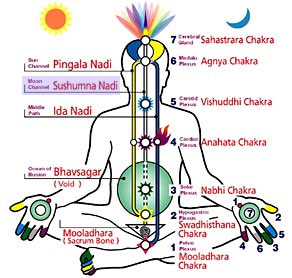
\includegraphics[scale=.5]{a20120823TheDivineJourney-img001.jpg} 
\end{wrapfigure}

Since we have recently been alluding to states of being, the path of the initiate, and postmortem states, we will start near the end with \emph{Chapter XXI: The Divine Journey of the Being on the Path of Liberation}. The final stages of this path assume that a man has reached a certain stage in development symbolized by the coronal artery (\emph{sushumna}) at the crown of the head and connected by a ray to the spiritual Sun. For casual readers, we point out here that any astronomical or elemental symbolism is not to be understood in the material sense.

The being must then follow the way marked by the path of this ray and retracing it back to its source, which is also identical with its destination. We can point out here, in passing, that this is also the esoteric meaning of the stories of Genesis and Exodus, which is repeated in Tradition: it represents the journey from the source to the fall, then to exile in the West and finally the return back to the source. Guenon reminds us that religious conceptions are capable of a transposition to a higher and deeper meaning, something we should always look for instead of rejecting exoteric teachings out of hand (or even accepting their basest interpretation).

This chapter does not deal with the \emph{jivan-mukti}, that is, the being who achieves Deliverance in the human state, but rather with two types of beings:

\begin{enumerate}
\item Beings who obtain Deliverance on leaving the human state 
\item Beings who pass into other states of individual manifestation 
\end{enumerate}
There are, therefore, two corresponding paths:

\begin{enumerate}
\item Path of the Gods (\emph{devayana}) 
\item Path of the Ancestors (\emph{pitriyana}) 
\end{enumerate}
Note that these two paths do not exhaust all the options for postmortem existence. Keep in mind, too, that these paths concern the subtle states of the being, which are still formal and individual, although the corporeal state is no longer part of the being.

Although there are some differences in the order or names of the stages, it may be helpful to compare this to the diagram in Spiritual Beings.

\paragraph{Path of the Ancestors}
Some will recognize this from the descriptions of the way of the ancestors in our series on the Ancient City. Its symbols are: Smoke, night, waning moon, the sun descending to the south. This path is restricted to the Sphere of the Moon\footnote{\url{https://en.wikipedia.org/wiki/Sublunary_sphere}}. Thus, the being is not set free from form or individuality.

The \emph{Sphere of the Moon} represents Cosmic Memory, or the Akashic Record. This is because it is inhabited by the beings of the preceding cycle, who then generate the current cycle. As forms complete the full course of their development, they are dissolved, becoming the germs of undeveloped forms. The end of one state is always the beginning of another.

Thus the being ends one state of existence and begins a new one as an individual in a world of form. Since a being does not occupy the same state twice, the new form does not exist in this world at a later date, as a crude understanding of reincarnation would have it. Nevertheless, it will be in a state of existence, perhaps similar to this one, depending on the possibilities attained in the previous state of existence. This idea is more fully developed in the \emph{Symbolism of the Cross}.

The Lunar Sphere separates the higher, non-individual, states from the lower. This is what separates the two paths. Guenon points to the Litany of the Virgin\footnote{\url{https://www.nashvilledominican.org/prayer/litanies/litany-of-the-blessed-virgin-mary/}} as representing this division, where we read,

\begin{quotex}
Who is she that comes forth as the morning rising, fair as the moon, bright as the sun, terrible as an army set in battle array? \flright{\textsc{Song of Solomon 6:10 }}

\end{quotex}
\paragraph{Path of the Gods}
This path represents those who tend toward Union never to return to manifested existence. Its symbols are: Fire, light, daytime, waxing moon, the sun ascending to the north.

In Vedic symbolism, after leaving the Earth or the world of gross manifestation, i.e., at death, the being is led to the Realm of light, or Fire, ruled by Agni. Then the being is led through the different stages of the \emph{devatas}. In Western symbolism, these stages are said to be ruled by angels. Note, too, that the principle of each stage is personified by a supernatural being. This is not at all insignificant.

Guenon points out that other traditions describe this path and he specifically names the Egyptian Book of the Dead, the Tibetan Bardo Thodol and the Alexandrian Gnostic text Pistis Sophia. He suggests a concordance be written between these texts. 80 years later, this has not yet been done by anyone. We would add to this concordance Ibn Arabi's Meccan Revelations and Dante's Divine Comedy.

As he progresses, the being effectively identifies with the center of the Personality, losing all individual concerns. The effective realization of each state is obtained through identification with the principles of the state. Theoretical knowledge is only a preparation. Transition from one stage to the next is possible only after effective knowledge of the stage. As formless, the being may pass to a Deva or angelic state.

The penultimate stage is the principle of Being, represented by Ishwara. At this point there is no longer any subtle state and the being is in an unmanifested state. The center of the being is identified with the center of all the worlds; this is the same as the fundamental analogy between the macrocosm and the microcosm.  This would persist until the end of the cycle. In Western terms, this is equivalent to Heaven.

\emph{Final Deliverance} is beyond Being, Infinity\footnote{\url{https://www.gornahoor.net/?p=3261}}, comprising Being and non-Being. That is why Guenon's Deliverance is usually called non-dual awareness. The being is liberated from the conditions of individual human existence and well as all other limiting conditions.

\paragraph{Theoretical Preparation}
Guenon provides us with the theoretical preparation for the path; to become gnosis, a man must realize it fully in his heart. Being and Knowing are one. It helps to think about or meditate on these ideas constantly until your entire worldview is permeated with them. Along with that, there is knowing one's true Self, or Atman. This is beyond the individual and is never manifested as such. A question to ponder is:

\textit{What is constant and unchanging in every act of consciousness?}

\flrightit{Posted on 2012-08-23 by Cologero }

\begin{center}* * *\end{center}

\begin{footnotesize}\begin{sffamily}



\texttt{Sparrow on 2015-03-14 at 02:48 said: }

I've been reading a bit about Guenon's view of what happens after death, and while it's logically consistent, I can't really see any reason it's true and the common understanding of reincarnation is false. Almost all ancient teachings that I can recall (Bhagavad Gita, Myth of Er, Bardo Thodol, etc.) don't even come close to suggest a being passes into another state of existence on another plane, never to return to this one. It seems that the opposite case is near universal. While I would be willing to accept that by the fifth century B.C., the ancient teachings had already devolved into reincarnation, Guenon explicitly states this is not the case and that the ancients held the view of transmigration how he describes it.


\end{sffamily}\end{footnotesize}

\section{Multiple States of the Human Being}

\begin{quotex}
Thou hast ordered all things in measure and number and mass. \flright{\textsc{Wisdom of Solomon 11:20}}

A science was less esteemed for itself than for the degree in which it expressed after its own fashion and represented within a certain order of things a reflection of the higher immutable truth which anything of any reality necessarily partakes of. \flright{\textsc{Rene Guenon}, \textit{East and West} }

\end{quotex}
\paragraph{Namarupa}

\begin{wrapfigure}{rt}{0.35\textwidth}
\centering
 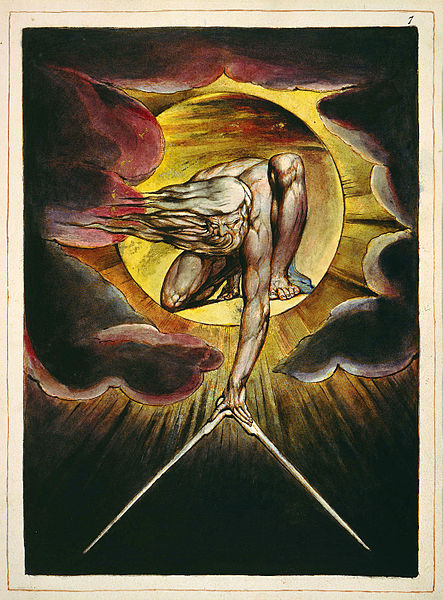
\includegraphics[scale=1]{a20200621MultipleStatesoftheHumanBeing-img001.jpg}
\caption{Ancient of Days}
\end{wrapfigure}

Moving on from Vaisesika to Advaita Vedanta, particularly as explained by \textbf{Adi Shankara}, we will focus on the teachings on the world of nature. Namarupa, literally meaning “name and form” constitute an object or being. They correspond to the intelligible and sensible aspects, or, in different words, “form and matter” or “essence and substance”. This shows why English is a poor language to express metaphysical concepts, since the words are not precise — “form” is used in two different senses.

Nevertheless, this concept is identical to Platonism and Scholasticism, which represent the peak metaphysics of the ancient and medieval Europeans. The point is that our experience includes the senses as well as thought. The experience is incomplete until the mind makes a judgment about what it is. Although the senses and thought are not one, there is no dualism of thought and extension in the Cartesian sense: it is nondual.

Everything that exists, has name and form. Physics, then, is the study of the world of matter, i.e., “becoming”, and Metaphysics, then, is the study of the world of ideas or essences, i.e., “being”. Apart from Adam, who was infused with an intuition of essences (he “named” the animals), we start with the senses and move on from there to an understanding of ideas. Hence, we can accept physics while rejecting the claim that science is the sole and exclusive form of knowing. Rather, properly understood, physics can illustrate metaphysical principles.

It is pointless to denigrate modern science, since the technological consequences of physics are all too evident all around us, for better or worse. Human flourishing cannot depend on the revival of “traditional” sciences like chiromancy (“palm reading”) or astrology. I have had my palm read and my natal chart interpreted — good fun, but limited applicability.

Vladimir Solovyov had a deeper understanding of things, as described in \textit{The development of mind}\footnote{\url{https://www.gornahoor.net/?p=3514}}. Science, philosophy, and theology are three forms of knowing, at increasing depths. Since, as Guenon claimed, time is not neutral, but is qualitative. This means that events occur at time periods that is proper for them, not at random or without sufficient reason. Hence, the notion of development in time a necessary consequence.

\paragraph{Elements}
The elements and their properties in Advaita are basically same as in the Vaisesika system, since both orthodox schools follow the Upanishads. These elements are qualitative and therefore not part of physics. Nevertheless, as was shown in the case of the element fire or light, it does have real world effects. Another example is the element Akasha, or ether, which fills empty space. Einstein famously rejected the existence of the ether since he understood it only in terms of physical matter. However, the Void, i.e., “empty space”, is not a possibility of manifestation. Nature abhors a vacuum. So we should not be surprised when physics find that the so-called vacuum is actually quite busy. See \textit{The Vacuum State}\footnote{\url{https://en.wikipedia.org/wiki/Vacuum_state}}, for example.

\paragraph{Atomism and Continuity}
God has ordered all things by measure, number, and mass. For the first two, we have these relationships:

Measure = geometry = continuous

Number = arithmetic = discrete or atomistic

Measure, as continuous, can be indefinitely divided. On the other hand, atoms are the smallest parts which cannot be further divided. Vaisesika holds the atomistic view whereas Advaita claims the other. Which is correct, since both systems are orthodox? If we turn to physics, we see that both are true. For example,

\begin{enumerate}
\item Light is both a wave – that is, continuous – and a photon, that is, an atom of light 
\item Electrons likewise act like waves or particles, depending on circumstance. 
\end{enumerate}
This can go on. Physics cannot explain this phenomenon, but metaphysics can.

\paragraph{States of Being}
Inorganic nature serves a purpose which lies beyond it; that is because it does not have its own self-organizing principle. The division of inorganic nature if somewhat arbitrary. Where does one mountain begin and another end? What are the precise boundaries of the oceans?

Organic things are likewise composed of the same elements as inorganic nature. In addition, a new principle comes into play: viz., the power of life. Life realizes a state of greater perfection through its power of realising an ideal. Here are examples of states of greater perfection, from lowest to highest.

\begin{itemize}
\item \textbf{Stone}. A stone does not live, since it has no tendency to become perfect, no inward inclination or strength to turn itself into a pillar or a statue.
\item \textbf{Plant}. A plant lives. If placed in suitable conditions, it has the power to grow, put forth leaf and blossom, flower and fruit. 
\item \textbf{Animal}. An animal is capable of a fuller life than the plant. It sees, hears and feels, and also knows vaguely what it is about. Not only does it thrive in favourable conditions, but it goes out to find those conditions. It moves on purpose, while the plant does not. 
\item \textbf{Human}. The human being lives a much higher life. He is a reflective being, with understanding and will. He has the growing power of the plant, the moving and the sensing powers of the animal, as well as the power to pierce behind the veil, discriminate the eternal from the non-eternal, choose between good and evil. 
\item \textbf{Angelic states}. Men who realise their ambition are the gods. 
\item \textbf{Jivanmukta}. The realisation of the Supreme Identity or Beatific Vision. Someone who has achieved self-realisation. 
\end{itemize}
Each state of being is ontologically different from the others. Just working out in the gym does not result in an ontological change, as some wannabe traditionalists have claimed. The human state encompasses all the lower states, but adds the intellectual soul. It should be obvious from the description that biology or evolutionary psychology cannot explain it.

The human state relies on rational thinking, which is sequential and therefore subject to time. When a man has realised his possibilities, he has reached an angelic state (“gods” as Radhakrishnan puts it). In this state, there is a direct understanding through intuition, which is immediate and beyond time. It is more like an “aha” experience than logical demonstration. This is the Edenic state, before the Fall. Thomas Aquinas describes it this way:

\begin{quotex}
In paradise man would have been like an angel in his spirituality of mind, yet with an animal life in his body. 

\end{quotex}
He goes into more detail about angelic states in \textit{Treatise of separate substances}\footnote{\url{https://isidore.co/aquinas/SubstSepar.htm}}.

Even beyond this state, there is the Beatific Vision, achieved by few. Aquinas elaborates on this description of the Beatific Vision or Supreme Identity:

\begin{quotex}
Man was happy in paradise but not with that perfect happiness to which he was destined, which consist in the vision of the Divine Essence. 

\end{quotex}

\paragraph{Appendix}
The study of the metaphysics or the Hindu schools does not mean that we have to accept the mythologies of the Ramayana or Mahabharata, apart from the Bhagavad Gita.

As should be clear, the Medieval and Ancient metaphysics of the West are equivalent to that of the East. Westerners can study Eastern systems either to enrich or recover Western tradition. Those Westerners who fail to recognize this and instead embrace in toto those of the East typically show their misunderstanding of both.

Some unacknowledged quotations are from Indian Philosophy, Volume Two, by \textbf{Sarvepalli Radhakrishnan}.

\flrightit{Posted on 2020-06-21 by Cologero }

\begin{center}* * *\end{center}

\begin{footnotesize}\begin{sffamily}



\texttt{Draft Horse on 2020-06-24 at 03:05 said: }

A good post, but I think you write off the traditional sciences too readily, especially astrology. 

In a “practical” sense, done properly it can identify a persons talents, and show them the most important days/times of their life, along with helping them avoid danger. 

More importantly, it can facilitate in the astrologer (who is suitably disposed) an easier understanding of higher metaphysical principles, particularly the ones written about in Symbolism of the Cross. Then there is also the alchemical usages, hinted at by Evola in his book on the subject. 

Of course astrology today has been co-opted by counter traditional forces, but it still has a capacity for higher use in the right hands, at least that's what I believe anyway. 

So, in short, I think it does have a great value for people today, especially those who are on a spiritual path.

A minor point in your post, but it caught my attention.


\hfill

\texttt{Cologero on 2020-06-28 at 09:54 said: }

I can't dispute your point in an absolute sense. Astrology at least recognizes that the time and place of one's birth is are necessary conditions of life, whereas the modern mind will typically consider them to be arbitrary and even unjust. Moreover, the planets are analogous to the subtle centers in the body. (See Oscar Hinze on Tantra Vidya\footnote{\url{https://www.gornahoor.net/?p=8618}}).

Whether there is benefit in a practical sense depends on the existence and availability of reliable astrologers.


\end{sffamily}\end{footnotesize}

\section{On Being a Person}

\begin{quotex}
The personality, let us insist once more, belongs essentially to the order of principles in the strictest sense of the word, that is, to the universal order; it cannot therefore be considered from any point of view except that of pure metaphysics, which has precisely the Universal for its domain. \flright{\textsc{Rene Guenon}, \emph{Man and his Becoming}}

\end{quotex}
Guenon noted:

\begin{quotex}
the conceptions of Aristotle are in complete agreement with those of the East.

\end{quotex}
With that in mind, we will use that as a guide to interpret not just Aristotle, but also Thomism as its extension. The goal is not to engage in an academic philosophical debate, but rather to explore how consciousness has altered from the Medieval period until now. We accept Owen Barfield's justification for focusing on Thomism:

\begin{quotex}
In the mind of Aquinas, with his enormous erudition, the whole corpus of medieval thought is in a manner recapitulated; and he is as sober as he is profound.

\end{quotex}
\paragraph{Person and Ego}
In this system, a human being is the individuation of a human essence into the corporeal world. That answers the question of “what” it is, but not who. Where then is the specific person, say Peter? Every substance has a \emph{suppositum} or center which, in the case of rational beings, is called “Person” (or Self or Spirit). Hence, Peter as person is also an essence, i.e., an idea in the Divine Intellect (Buddhi). Guenon relates the Person to its manifestation:

\begin{quotex}
The personality is unmanifested, even insofar as it is regarded more especially as the principle of the manifested state

\end{quotex}
In practical terms, this means

\begin{itemize}
\item The Person always exists as the principle of manifestation 
\item The Person cannot be detected by any empirical, physical, or psychological test. 
\end{itemize}
The Person transcends psychical and corporeal manifestation. You are not a “spirit in the world”, rather, you are in the world but not of it. You cannot “contact” the higher self. Conclusion: every human is a Person, even if only virtually (i.e., unaware of his real nature).

Contemporary thinking confuses the Person with some psychological state, ignoring

\begin{quotex}
the fundamental distinction between the `Self'. which is the very principle of the being, and the individual `ego'.

\end{quotex}
The Self, or Person, as intellect, is in the spiritual realm whereas the Ego is part of manifestation. Although claiming a pedigree from Aristotle or Thomism, they are not comprehending its source. This is not a failure of a convincing argument, but rather of the inability of consciousness in a give state to even grasp it. Guenon here points out that Aristotle did grasp it:

\begin{quotex}
For Aristotle, pure intellect is of a transcendent order and can claim knowledge of universal principles as its proper object; this knowledge, which is not discursive in any respect, is acquired directly and immediately by intellectual intuition.

\end{quotex}
This directly acquired, not-discursive, knowledge is called “knowledge of the heart”. This is opposed to a lower form of knowledge that is mediated by sensual images, or even thoughts:

\begin{quotex}
[Aristotle] said that man [as an individual] never thinks without image.

\end{quotex}
\paragraph{States of Being}
Contemporary philosophy restricts the Person to the human state, for the reason stated above: the Ego is assumed to be the Self. This is a failure to understand the medieval texts.

Dante, who claimed to be following Thomas, certainly knew other states of being. There are the subhuman states of hell, states in purgatory, and more famously, the transhuman states of the planetary, celestial, and angelic spheres. Ultimately, he was aware of heavenly states.

\paragraph{Metaphysical Realization}
In “The Eternal Ideas” from \emph{Miscellanea}, Guenon brings up the common misunderstanding that there is a distinction between the possible and the real, by regarding the unmanifested possibilities as merely \textbf{virtual}. Guenon makes clear:

\begin{quotex}
There can be nothing virtual within the Principle but, on the contrary, only the permanent actuality of all things in an `Eternal Now'. and it is this very actuality that constitutes the sole foundation of all existence.

\end{quotex}
The Self “always remains unmanifest, not being affected or modified by any contingency.”

This clearly indicates that there is no psychological explanation of the Self because it transcends all phenomenal reality. The Self remains virtual, that is, a mere intellectual concept, until there is a consciousness of oneself as that Self. G concludes:

\begin{quotex}
From the moment one recognizes that the existence of manifested beings in all their positive reality can only be a participation in principial Being, there cannot be the slightest doubt about this matter. … \textbf{What is virtual is not our reality within the Principle, but only the awareness we may have of it as manifested beings}, which is obviously something quite different; and \emph{it is only through metaphysical realization that this awareness of our true being, which is beyond and above all becoming can become effective}, that is actualized in the awareness … an awareness of that which we really are principially and eternally, and \emph{this is in the most absolutely real sense possible}.

\end{quotex}
Barfield explains it this way:

\begin{quotex}
Participation ceases to be conscious precisely because we cease to attend to it. … participation does not cease to be a fact because it ceases to be conscious. It merely ceases to be what I have called `original' participation.

\end{quotex}
The corollary is that ignorance is just “forgetting”, we cease to be conscious of what we know. As the following discussion shows, we can even be ignorant of our true Self. So \textbf{virtual} does not mean \textbf{unreal}, rather it is tantamount to unawareness or, in Barfield's term, unrepresented. Yet what is virtual still exists, one is simply unaware of it.

\emph{So the more you can become conscious of, the closer you are to, the true Self. Don't forget}.



\flrightit{Posted on 2021-09-30 by Cologero }

\section{Principles of Manifestation}


\begin{wrapfigure}{rt}{0.35\textwidth}
\centering
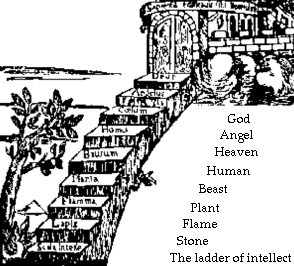
\includegraphics[scale=.5]{a20141119PrinciplesofManifestation-img001.png} 
\caption{Great Chain of Being}
\end{wrapfigure}
 
If cosmology is the study of the origin, nature, and destiny of the universe, there have been many conflicting theories. In the West, the basis of cosmology has been what is called the \textbf{Great Chain of Being}. In various versions, it has formed the worldview of educated people until recently. The dominance of profane science has done much to discredit it, even to the point that exoteric spiritual teachings not only neglect it, but in effect oppose it. This often has less to do with science than with ideology.

The Great Chain of Being is based on certain Traditional metaphysical principles. These need to be made clear, but first the implicit principles of modernity must be made clear.

\paragraph{Profane Worldview}
In its most consistent form, the modern worldview is based on the notion that the origin, nature, and destiny of the universe can be fully explained in terms of matter and energy. Obviously, this worldview denies that there is a world of Being ontologically prior to, and superior to, the world of Becoming. Profane science needs to explain:

\begin{enumerate}
\item How emergent properties such as life, mind, consciousness, emotions, thought, in short, interiority, evolve from material and exterior processes. 
\item How higher order systems are constructed from more basic elements. 
\end{enumerate}
Thus far, science has no answer to issue (1), not even a plausible theory. Issue (2) is often hidden in popular discourse. Profane science is committed to reductionism, viz., higher order systems are fully explicable by more fundamental elements. By denying the existence of essences or forms, the task of science is to define higher systems; in its most consistent philosophical expressions, these are mere “social constructs”.

\paragraph{Evolution and Involution}
\textbf{Rene Guenon} explains that there are five conditions of manifestation: space, time, form (or essences), matter, and life. The opposite of “evolution” is not creation science, or even intelligent design, but rather involution.

Evolution is the notion that simple things evolve into complex structures caused by random variations over time. Involution is the notion that ideal essences are brought into manifestation by a will. Depending on the strength of the will, the existing being will be a better or worse copy of its ideal.

Essences unfold in space and time, thus appearing to be evolving (e-volve = unfold), but really involving. For example, Beethoven's Ninth Symphony is an “idea” or essence. However, to be experienced, musicians and instruments are necessary for the symphony to unfold in time. Profane science has nothing to offer. It makes no sense to say that the first movement “causes” the final movement. A fortiori, it is risible to try to experience or understand the symphony from an analysis of its individual notes.

Hence, Guenon claims that the higher order system defines its components, rather than the other way around. The other point is that “life” is prior to matter. So, in a sense, everything is “alive”, that is, it has interiority. Hence, esoterism understands the cosmos as an interior process, unlike an astronomer who takes the opposite approach.

\paragraph{The Idea of the Good}
Plato understood God to be the Idea of the Good. Hence, man's goal is to passively contemplate the Good. The Christian notion of God as Love builds on that, since Love means to will the good. It is a revealed truth that the created world is “good”, so the good is whatever has more being. The goodness of God, then, is His creative activity. So to be godlike is also to be creative, in the sense of bringing essences into manifestation. The gap between the essence and its existence is privation, i.e., “evil”.

\paragraph{Rationality and Intellectuality}
Rationality is the quality that distinguishes man from animals; intellectuality distinguishes God from man. Rationality involves dualist thinking, but intellectuality is non-dual. It is not irrational, but rather super-rational. Any attempt to conceive of God's knowledge and will in rational terms will fail. For example, I read on a web site a few months back the claim that “God knows all true propositions.” Not at all, God knows the Divine ideas directly and non-dually, not as propositions. He “knows” the world because He created it. There is not duality of essence and existence for God.

Similarly for the Divine Will, there is no distinction between freedom and necessity. God does not “deliberate”, choosing this or that, but rather whatever exists is the expression of his Goodness. Some will claim that God cannot do things like creating a square circle. It is better to understand that as a possibility of non-manifestation. There are four such possibilities.

\begin{enumerate}
\item \textbf{Analytic}. The definition contains a self-contradiction (as in the example above). 
\item \textbf{Synthetic}. The contradiction is not in the definition. “A colored thing must also be extended.” 
\item \textbf{Physical}. The human frame has an upper limit, since as an increase in height is linear, the increase in mass is cubic. Hence, the skeletal structure will not be able to support that weight. 
\item \textbf{Compossibility}. Certain possibilities of manifestation cannot manifest in the same place or time 
\end{enumerate}
The loss of intellectuality in the modern world has consequences. First of all, rationality tries to take its place; it is doomed to failure. The next step is that emotionality, i.e., the subrational, as a sort of non-dual experience, usurps the place of true non-dual intellectuality. Hence, Love is understood not as the creative Will to being, but rather in a sentimental and humanitarian way as compassion and the alleviation of suffering.

The modern mind misunderstands evil and thinks there is a “problem of evil” to be explained. However, the teaching is that creation is good, so that the world of good and evil that we experience is the creation of man. If the cheetah chases the gazelle, the result is good for the cheetah since it increase his being, but bad for the gazelle since his being is ended; however, there is no question of “evil” in that scenario. On the contrary, it is good that the gazelle was given being in the first place.

\paragraph{Principle of Plenitude}
In the \emph{Multiple States of Being}, Rene Guenon showed that the Absolute must also be Infinite, that is, the number of possibilities is unbounded. He formulated the Principle of Plenitude as “All possibilities of manifestation must be manifested.”

This accounts for the immense variety in the world. Every creature has its place in the chain, or scale, of being. It is irrational to expect everything to be the same, so the scale is hierarchically arranged. Moreover, there are many more scales of being than the one that describes our world.

\paragraph{Principle of Continuity}
A related principle is the Principle of Continuity, described in the \emph{Metaphysical Principles of Infinitesimal Calculus}. The gaps in the scale become arbitrarily small. Thus, we see that a taxonomic problem arises in biology, since it can become difficult to distinguish between closely related species and subspecies. Hence, there is no absolute definition of a species. That problem is insoluble as long as biological and material considerations are the only criteria used. In such a case, definitions are considered arbitrary social constructs.

Of course, the Traditional view is different. These close differences nevertheless reflect different essences in the Divine mind. Proper classifications will have to take the soul and spiritual elements (i.e., “interiority”) into account. Hence, the differences are real, no matter how close they may appear. There are some further points that can be derived from this principle, although they cannot be fully developed in this post:

\begin{itemize}
\item The attempt to refute Darwinian evolution by pointing to “missing links” in the fossil record (yes, the term is derived from the Great Chain of Being) is actually anti-Traditional. 
\item The Great Chain of Being is a simplification. It is better represented as scales within scales. 
\item \textbf{Otto Weininger} in \emph{Sex and Character} defines the ideal masculine and feminine qualities. However, they don't manifest in a strictly binary way, but rather on a scale ranging from absolute femininity to absolute masculinity. 
\item Intellectual movements always ramify into two competing camps whenever the possibility of a dispute arises. For example, a predestinarian Baptist church will give rise to a “free-will Baptist church”. In other cases, movements will split by incorporating elements from other, often incompatible, movements. This is why all movements are prone to degeneration and inner conflict. 
\end{itemize}
\flrightit{Posted on 2014-11-19 by Cologero }

\begin{center}* * *\end{center}

\begin{footnotesize}\begin{sffamily}



\texttt{Constantine on 2014-11-19 at 14:25 said: }

Reading through this article I felt something was missing. You make a good point fractal, what about energy (chi, prana…)?


\hfill

\texttt{Francesco on 2014-11-19 at 16:14 said: }

Constantine: Imo, Qi can be handled under the five conditions of manifestation, some more than others Perhaps in the same way that Sophia is not a fourth hypostasism but the life shared in common by the trinity; Qi is not another condition, but something shared commonly among form, matter, and life. 

In Chinese metaphysics, there are a great number of “Qis”: human body qi (then specific organ and system qi types), cosmological qi (astrology), environmental qi (feng shui), and so on. To see how better how this concept is subsumed in the five conditions, we might consider the famous Chinese character for Qi–which is a pot of rice gruel cooking, with steam raising from the vessel lid–it is interpreted as “it moves”, or “acts”.

The Classics explain “Qi is the commander of Blood; Blood is the mother of Qi”, and that “Qi follows where the Shen (consciousness) leads”.


\hfill

\texttt{Cologero on 2014-11-19 at 17:37 said: }

@Constantine: “Matter is condensed energy and energy is condensed consciousness.” \flright{\textsc{Valentin Tomberg}}


\end{sffamily}\end{footnotesize}


\chapter{Macrocosm and microcosm. Layers of the soul}
\section{Prequel to the Three Worlds}

\textbf{Cornelius Agrippa}, in \emph{Occult Philosophy}, posited the existence of three worlds: the elementary, celestial, and intellectual worlds, hierarchically arranged, as illustrated, for example, in \textbf{Robert Fludd}’s Diagram\footnote{\url{https://www.gornahoor.net/wp-content/uploads/2011/03/hierarchy.jpg}}.

\begin{quotex}
Since each inferior world is governed by its superior and receives its influence, so the mages believe that one can penetrate naturally by means of the same levels and for each one of these worlds up to the “archetypical world”, constructor and ruler of all things and from there to act not only on natural powers, but to also create new ones.

\end{quotex}
In the essay on \textbf{Hermann Keyserling}, \textbf{Julius Evola} added that as a footnote to some of Keyserling’s ideas, in particular, “The representation creates reality, not vice versa.” Clearly, both Keyserling and Agrippa recognize that the subtle rules the dense. At this point, it is worth the time to consolidate the ideas about the three worlds.

Other terms for the three worlds are “hylic, psychic, and pneumatic” or “exoteric, mesoteric, and esoteric”. I was going to summarize these worlds in a post, but it became too long and involved. So, first there is this prequel which serves as the introduction.

\paragraph{What Is Spiritualism}
I recently saw part of a movie, which I don’t recommend: you will meet a tall dark stranger. In it, the ditzy mother, a divorcee, met a man she described as “spiritual”, because he dabbled in séances, reincarnation, psychics, etc. Obviously, that is quite far from what we mean by spirit. Rather we mean interiority.

That is the heart of the Western tradition, also called “spiritualism” in other languages, but, unfortunately, that has much different connotation in the Anglosphere. So we are forced to use the term “idealism”. As we have pointed out many times, Plato is but one link in a long chain that goes back much further than him. It took different forms in 19th century Germany, moved on to France and Italy, where the trail goes cold in the second half of the 20th century.

In the mission to contribute to the living stream of Hermetism, it is imperative to revive this way of thinking. At a time when materialism and positivism are seen as the touchstones of rational discourse, the spiritual worldview may seem incredible. Nevertheless, an intellectual conversion is possible, in which case it will be understood as the most sane and intelligent view. Since Julius Evola consciously attempted to tie European idealism to Hermetism, his system of magical idealism is worthy of study.

For more background, I suggest reading through The Science of Peace by \textbf{Bhagavan Das}\footnote{\url{https://www.gornahoor.net/library/ScienceOfPeace.pdf}}, reviewed by Evola\footnote{\url{https://www.gornahoor.net/?p=6328}}. He connects Advaita Vedanta to German idealism, particularly Fichte.

\paragraph{Macrocosm}
Whenever some people hear of “occult philosophy”, “magic”, or “mages”, they tend to shut down, visualizing something heretical, dangerous, or even satanic. However, properly understood, it is the consequence of orthodox teachings. The purpose of exoteric practices is to create certain states of consciousness, although in a spontaneous and passive way. So a particular devotion may lead to one such state or another. As spontaneous, it is experienced by the practitioner as originating from the outside.

The esoterist, on the other hand, achieves the same states in an active way, as the free act of the will. He does not oppose the exoterist, but rather understands the teachings in a very different way. This can be revisited after the commentary on Keyserling on the topics of understanding and meaning. Since the exoterist cannot understand the esoterist, he assumes there is something false about it.

Another difference is the relationship to ideas. The exoterist uses ideas more as weapons to buttress an argument or to win debates. For the esoterist, an idea is a real, active, and living force. So let’s take the idea of the three worlds into consideration. Basically, it is saying that the Divine creates the order of the universe, the angelic hierarchies are charged with the maintenance of that order, and the elementary world, i.e., the phenomenal or natural world, is the result. This is the principle that the subtle rules the dense on the macrocosmic scale.

The exoterist agrees with that, but sees it as something happening from the outside, with no further relevance. The Mage, as Agrippa points out, instead understands that teaching interiorly and then strives to “penetrate” into those levels. There is certainly justification for this. Since God and the angels are spiritual beings, there is no “outside”. Either they are known interiorly or else the possibility of gnosis is denied a priori. Those who have experienced gnosis know the answer.

\paragraph{Microcosm}
The analogy of being —as above, so below— is also orthodox. So corresponding to the three worlds in the microcosm is the spirit, the soul, and the body. These are definitely experienced interiorly. And they functionally correspond to Agrippa’s three worlds. The spirit rules the soul and the body. The body is not independent; the spirit and soul are the form of the body. Hence, any mage who can penetrate into the knowledge of the inner workings of the spirit and soul can then have control over the natural world as represented by the body. This can even happen spontaneously in various psycho-somatic manifestations.

The point here is not a scholarly discussion of Agrippa, but rather to come to experience these teachings from the inside.

\paragraph{The Thirst for Action}
\textbf{Theophan the Recluse} pointed out that there are three stimuli that motivate the thirst for action:

Stimulus $\rightarrow$ Object of desire

The Necessary $\rightarrow$ Duty

The Useful $\rightarrow$ Service

The Pleasant $\rightarrow$ Pleasure

He writes that there are natural and legitimate activities of the will,

\begin{quotex}
which is the master of our powers and our whole life. Its work is to determine the form, the means and the degree of satisfaction to be given to the different desires that arise from our needs, and to decide on substitutions so that life may flow smoothly and bring peace and joy to the individual.

\end{quotex}
The high-functioning Will, then, will balance the natural needs that relate to the sour, the body, everyday life, and to society. Unfortunately, the Will can be dissipated and “alien things stimulate desires that are foreign [unnatural] to us: anger, hatred, envy, miserliness, vanity, pride, etc.”

\paragraph{Active Spirituality}
The last time, I contrasted two spiritual perspectives:

\begin{itemize}
\item The desire for worldly things 
\item Detachment from the world 
\end{itemize}
As such, they are both passive approaches, so what happens if we flip them around as active forces. Two things result from that. Rather than being two distinct incompatible approaches, they instead become complementary.

\begin{enumerate}
\item The prayers for worldly successes turn into the work of the mage to penetrate the archetypal world of ideas in order to bring them into manifestation. However, the desired manifestations should conform to our natural needs arising from our sense of duty, the utility of the manifestation, and legitimate pleasures. 
\item Yet, there is detachment from the world and the results of our willing as described in the fruits of mental prayer. 
\end{enumerate}
As Theophan concludes, all is done for the greater glory of God. The Warrior-Monk will have complete confidence that his Will is in conformity with the Divine Will and his prayers will be answered. Yet he is also detached from the world.

\flrightit{Posted on 2014-07-28 by Cologero}


%. Pagan views, Vedanta, the place of Christianity
% La llegada al Ser desde distintas tradiciones
% (continúa la escala del Ser)
%intersección entre filosofía y metafísica: moral: cómo vivo y me afectan los primeros principios
\chapter{The trascendent unity of religions}
\section{The Knowledge of God}

The transcendental unity of religions is true insofar as it pertains to metaphysics. In Lecture 6 of \emph{Lectures on Divine Humanity}, \textbf{Vladimir Solovyov} shows his agreement with that point even for Christianity. In particular, he writes this about Neoplatonism:

\begin{quotationx}
It is impossible to deny the connection between Philo's doctrine and Neoplatonism, on the one hand, and Christianity, that is, precisely the Christian doctrine of the Holy Trinity, of the triune God.

The first speculations concerning God and His inner life by such Christian teachers as Justin the Philosopher, Hippolytus, Clement of Alexandria, and especially Origen reproduced the essential truth of the doctrine of Philo and Neoplatonism. 

\end{quotationx}
Furthermore, Solovyov traces this connection all the way back to the Egyptian theosophy of \textbf{Hermes Trismegistus}. This is because metaphysics deals with essences, but it is fair to ask if that is exhaustive, when it comes to existing things. \textbf{Rene Guenon} skirts around this is his notion of possibilities of manifestation. In that sense, an existing thing, or manifested possibility, is metaphysically no different from a possibility of non-manifestation. This seems to be what \textbf{Aristotle} is saying when he claims that God does not know particular things.

\textbf{Julius Evola} disputes Guenon on this point. As we saw in the discussions on the Individual and the Becoming of the World, to become manifest, an idea requires an act of will. As such, the individual is not an object of contemplation. Evola thought he was opposing action to Guenon's contemplation. However, they are not in opposition, since they are united under the “Person”, who is both the center of contemplation and of will. As we shall see, Evola was not recovering pagan ideas as he believed, but was actually recuperating Christian ideas.

\paragraph{The Pagan and Contemplation}
The fundamental revelation made to the rishis in the Vedas was the existence of a higher self and that the manifest world was the result of ignorance, or avidya. The solution, then, was to dissolve the lower self, as knowledge of the higher self was itself liberation. That knowledge is the end of ignorance. This higher self then passively observes the passing phenomena of the world. However, this involves the dissolution of the person, because there is no longer a will. The self does not create the phenomena, but merely observes.

This solution is carried into Buddhism. It deepens the Vedic revelation when it sees suffering as inherent in the phenomenal world and it ties this suffering to desire. The Buddhist solution is therefore the elimination of desire, or the will. Again, the person is denied by following this path, since a person has will by definition.

For the Greeks, too, the highest life was contemplation. Like the rishis, ignorance was the cause of suffering and ignorance was removed by knowledge of the self. This knowledge would lead to “justice”, or the proper arrangement and relationship of the various parts of the soul to each other. The world, then, was contemplated as an object.

\paragraph{The Christian Revelation}
Among the world's traditions, Solovyov explains the distinctiveness of the Christian Tradition:

\begin{quotex}
The originality of Christianity lies not in its general [metaphysical] views, but in positive facts, not in the speculative content of its idea but in its personal incarnation. This originality cannot be taken away from Christianity, and to affirm it, one does not need to try to prove, against history and common sense, that all the ideas of Christian dogmatics appeared as something absolutely new, that they fell, so to speak, ready-made from heaven. 

\end{quotex}
Solovyov explains the relationship between a person and an idea. Without a subject to actualize it, an idea would be passive and impotent. It could not really exist. To achieve real, full being, the inner unity of person and idea is necessary.

By analogy, the absolute idea is also determined in its inner subjective existence as a particular and unique person. This insight requires a living God, God as a fact, not the passive Brahman. The living God reveals Himself as “I am”, not with respect to particular things but with respect to the All, or the Infinite.

Still, the initial revelation to the Hebrews was incomplete and partial. They saw God's will as arbitrary in Himself, but compulsory for humanity. But the understanding deepened, and the will of God could not be understood as despotism, but rather as the consciously chosen good. For the person, the compulsion is experienced as internal necessity, i.e., true freedom. Hence, the path of salvation, or liberation, is not the annihilation of the will as in the various forms of paganism, but rather the alignment, or better submission, of the personal will to the divine Will. Since God is Absolute and Infinite, there can only be one such Will.

So on the one hand, there is the revelation of the absolute personhood of God made to the Hebrews. On the other, the absolute idea of Divinity was grasped in Greece. The complete knowledge of God requires the synthesis of both these elements. That was the task of Christianity.


\hfill

\flrightit{Posted on 2014-04-02 by Cologero }

\begin{center}* * *\end{center}

\begin{footnotesize}\begin{sffamily}

\texttt{Michel on 2014-04-03 at 13:41 said: }

“Hence, the path of salvation, or liberation, is not the annihilation of the will as in the various forms of paganism, but rather the alignment, or better submission, of the personal will to the divine Will. Since God is Absolute and Infinite, there can only be one such Will.”

I have a question, when you say “personal will” do you mean individual? Or do you mean Personality, as in Atma?Assuming you mean individual: so whether or not one's individual will subsists doesn't really matter, because God's Will happens anyways. Whether the individual aligns himself to it and does not experience anything higher than his individual self, or whether he goes beyond it (annihilation as a term to describe this happening is rather misleading, because it implies a loss of something and hence a limitation on the higher station that the being would achieve;synthesis would be a better term, the principal of the individual doesn't deprive him of his individuality, because, being its principal, it has synthesized it in itself) doesn't affect this. 

“By analogy, the absolute idea is also determined in its inner subjective existence as a particular and unique person. This insight requires a living God, God as a fact, not the passive Brahman. The living God reveals Himself as “I am”, not with respect to particular things but with respect to the All, or the Infinite.”

As you have said in your article, there are Possibilities of non-manifestation that are non-manifest-able in accordance with their nature and there are those that are manifest-able being Possibilities of manifestation. They are “passive” insofar as they are Possibility and they are “active” insofar as they are Infinity. Possibility and Infinity refer to the “passive” and “active” “modes” of the Infinite. To use an analogy, Dave is man. Dave can jump, run, sing, shout, sleep and so on. Dave's existence therefore necessitates/affirms jumping, running, singing, shouting, sleeping and so on. Dave encompasses all these possibilities simply because he exists and those are the possibilities that are in concordance to his nature; in his passivity, Dave still “emanates” running, jumping, sleeping etc. If Dave jumps, runs, sings, shouts and sleeps at the same time, then Dave would have instantaneously actualized all the possibilities that his existence necessitates in accordance with his nature. So when you say, “This insight requires a living God, God as a fact, not the passive Brahman” are you referring to the Infinite in its “Passive Mode”, viz Possibility?

Consciousness is the sufficient reason for the perception of a state of being. I can perceive this state of being, because I am conscious of it. Destiny is the sufficient reason for the persistence of a being in individual mode. I am here because I have a destiny here. To go beyond one's destiny would be to realize it, by harmoniously synthesizing all the individual modes of existence that exhaust one's destiny. To perfectly and wholly do so, would be to align oneself with Providence and hence realize the Divine Will in relation to oneself. But would one have realized the Divine Will for that which lies beyond oneself and individuality? If so, wouldn't this be a virtual realization, still tied to the cosmological perspective? My question is, why stop there? Why not go beyond one's individuality wholly? Why not Realize the Divine Will that is truly Metaphysical, beyond both the formal and formless states of Being? Beyond the soul and the Spirit? Why not realize the Person, and hence perfect the realization of the Divine Will? If the Entity/Unraveled Archetype possess in itself something that entitles it to supra-individuality, nay to even supra-manifestation , supra-spirituality, true Metaphysics, why not actualize that something and realize this?

I really mean these questions; I am not the type of person to be insincere, so do not take these the wrong way. Forgive me beforehand if they are vague and want of clarity; and if they show a misconstrued understanding of this post and theme in general.


\hfill

\texttt{Cologero on 2014-04-03 at 21:40 said: }

I'm not sure what you are getting at, Michel. We understand by “person” a being with consciousness and will; the individual is more vague. Atma is consciousness, but how can the Atma be a person? That is the fundamental point of the essay. If God's will happens anyway, then why do we pray “Thy will be done, on earth as it is in heaven”?

I don't know why I need to repeat in a comment what was already written, but if a “person” loses his will, then he is no longer a person … that is an annihilation. Our point, however, is that the person cannot be annihilated, as he is immortal. The highest state is “liberation”, i.e., total freedom, i.e., absolute self-determination.

The pagans all regarded knowledge as the solution. Even Socrates said the the virtues would follow from knowledge. We know, however, that the moral problem arises in the will. A few weeks ago, a commenter claimed something similar. When I pushed her for the reasons why enlightenment, as she conceived it, could not be taught, she replied with a list of moral failings of the will. I pointed that out to her, and she chose to vanish.

You described Dave in his animal nature; that is not the actualization of his possibilities as a man. That actualization is theosis, becoming fully conscious and fully free. How you and I differ is that I am using precise language to describe the states you mention, while you are just singing in the rain.


\hfill

\texttt{Michel on 2014-04-04 at 02:07 said: }

This is what I understand by Personality:

”

The personality, let us insist once more, belongs essentially to the order of principles in the strictest sense of the word, that is to the universal order; it cannot therefore be considered from any point of view except from that of pure metaphysics, which has precisely the Universal for its domain.

”

“If a person loses his will, then he is no longer a person.”

So the defining aspect of a person is his will. Well, as I understood it, the Personality/Self/Atma is:

”

Is the Transcendent and Permanent Principle of which the manifested being, the human being for example is only a transient and contingent modification, a modification which, moreover, can in no way affect the principle…

The Self as such is never individualized and cannot become so, for since it must always be considered in the aspect of the eternity and immutability which are the necessary attributes of Pure Being, it is obviously not susceptible of any particularization, which would cause it to be `other than itself'. Immutable in its own nature, it merely develops the indefinite possibilities which it contains in itself from a relative potency to act through an indefinite series of degrees. Its essential permanence is not thereby affected, precisely because this process is only relative

and because this development is strictly speaking, not a development at all, except when looked at from the point of view of manifestation, outside of which there can be no question of succession, but only a perfect simultaneity, so that even what is virtual in one aspect is found to be realized in `the eternal present'

”

[Man and his becoming according to the Vedanta, Rene Guenon]

Thank you for clarifying that you were not referring to the individual, but to the Supreme Identity, when you said “personal will”. (That was all I was asking really, the other bulk of the comment was developed under the assumption that you meant one's individuality).

By will, I understand: 

“Immutable in its own nature, it merely develops the indefinite possibilities which it contains in itself from a relative potency to act through an indefinite series of degrees”.

Hence realizing the Self would imply realizing Will; and because the Self is

“the Transcendent and Permanent Principle of which the manifested being, the human being for example is only a transient and contingent modification”, then nothing is lost because all would be: “found to be realized in `the eternal present'” in concordance with the Will of the Self.


\hfill

\texttt{August on 2014-04-04 at 20:17 said: }

” If God's will happens anyway, then why do we pray “Thy will be done, on earth as it is in heaven”? ”

A better way to penetrate the issue: Do you propose that there is a single event anywhere in the Universe that occurs against God's Plan?

The quoted question invites confusion between the `personal God’ (demiurge) and the Absolute (sum of all disorders); the aspiring student of metaphysics should take pains to differentiate the two.

Further, even in a prayer, that statement can be read as an assertion rather than a plea.


\hfill

\texttt{Cologero on 2014-04-06 at 16:08 said: }

August, your response invites confusion between God's Will and God's Plan, which presumably you claim to be privy to.

Aspiring students of metaphysics should take pains to actually read a text, learn to think organically, and avoid abstract, mechanical thinking.

For example, to understand the points raised, he may want to read what Rene Guenon wrote about Providence, Will, and Destiny in the Great Triad. Providence is the reflection of God's Will … we have touched on this topic on many occasions.

The aspiring student may also want to read \textit{Freedom and Power}\footnote{\url{http://www.meditationsonthetarot.com/freedom-and-power}}. Then he could find the post where we quote Julius Evola that the way to know God is to be god. That is, theosis. In organic thinking, there are lot of pieces that need to be tied together, and I mean in one's interiority, not in some artificial metaphysical formulation.

So the best way to know God's will is to actually do God's will … then you will be a man who knows and you will have some authority.

Now, more advanced students may go back a week or two to the discussion of Shankara. If the world we experience is the result of ignorance, or avidya, then that cannot be God's will. Ignorance is not real, but is just a privation of knowledge.

Do you see how things ramify for the student of metaphysics? He needs to balance all the ideas in his head and make them a living realtiy, not an intellectual showcase.


\hfill

\texttt{Synodius on 2014-04-06 at 19:07 said: }

`If the world we experience is the result of ignorance, or avidya, then that cannot be God's will. Ignorance is not real, but is just a privation of knowledge.'

Our usual experience of the world is the result of ignorance (avidya) and so we cannot see it as God's will. With real knowledge we can see the world as it really is, which involves seeing it now comparatively less real (with different metaphysical status) than we did while in the state of ignorance. 

Can it be just different terminology and stress for different points of view or really a fundamental flaw in eastern views?


\hfill

\texttt{Cologero on 2014-04-06 at 23:04 said: }

Synodius, I assume you are making the point that their is a higher principle uniting Providence, Will, and Destiny. But, before getting to that, it does not change the fundamental point that Providence is the instrument of God's will. As above, so below: these three terms correspond in man to the intellectual, psychic, and instinctual forces, i.e., spirit, soul, body (see Guenon). So from below, the man who lives through his spirit, or intellect, corresponds to living under Providence (the subtle rules the dense).

So the uniting principle is knowledge of the Self. From below, the “I” unites the three forces. From above, God is the unifying principle. Nevertheless, Providence is the instrument of his Will, just as for a (true) man, the intellect is the instrument of his personal will. If you want to insist that whatever happens is God's will then you explain and understand nothing. It is the night where all cows are black.


\hfill

\texttt{August on 2014-04-07 at 07:31 said: }

Focussing on Providence, do we not again descend from the Absolute to the manifested? I challenge any participant to differentiate the Divine Will and the Divine Plan for us sub specie aeternitatis.

It is sad that the probing of metaphysical certainty seems to you mechanical.

And what alternative to believing that everything happens only by the Will of God? The Poor man confirms his faith, so be gracious and expose the flaw better if you see it.

James 4, 12-15, KJV:

“There is one lawgiver, who is able to save and to destroy: who art thou that judgest another?

Go to now, ye that say, To day or to morrow we will go into such a city, and continue there a year, and buy and sell, and get gain:

Whereas ye know not what shall be on the morrow. For what is your life? It is even a vapour, that appeareth for a little time, and then vanisheth away.

For that ye ought to say, If the Lord will, we shall live, and do this, or that.”


\hfill

\texttt{scardanelli on 2014-04-07 at 11:18 said: }

Sad also are missed opportunities for understanding. The light shines in the darkness, and the darkness comprehends it not. To truly probe metaphysics, to comprehend the light, keep thy mind in darkness. As long as we eat from the tree whose fruit is death, we will only play at knowing…we will only be pretenders chasing after imaginary forms and phantoms.


\hfill


\end{sffamily}\end{footnotesize}


%Esto en microcosmo:
\section{Subration}

I recently pulled out a couple of old books and notes from a box packed up years ago. One is \emph{Advaita Vedanta: A Philosophical Reconstruction} by the philosopher \textbf{Eliot Deutsch}. In reformulating Vedantic metaphysics in Western categories, he brings up some useful points. One is the idea of “subration” which he uses to translate the Sanskrit term \emph{badha}. He defines it thus:

\begin{quotex}
\emph{Subration} is the mental process whereby one disvalues some previously appraised object or content of consciousness because of its being contradicted by a new experience. A judgment about something is contradicted by a new experience when it is impossible to affirm both the previous judgment and what is learned or acquired in the new experience. … An object or content of consciousness is \emph{subrated} or \emph{subratable} when it is or can be disvaluated, denied, or contradicted by another experience. 

\end{quotex}
He applies that definition to different levels of being as described in the Vedanta.

\begin{itemize}
\item \textbf{Appearance} is that which can be subrated by another experience. 
\item \textbf{Reality} is that which cannot be subrated by any other experience. 
\item \textbf{Nonbeing} is that which neither can nor cannot be subrated by other experience. 
\end{itemize}
Subration involves:

\begin{enumerate}
\item A judgment about some object of content of consciousness (thing, person, place, condition, idea) 
\item The recognition, in the light of another kind of judgment that is incompatible with the initial judgment, that the initial judgment is faulty 
\item The acceptance of the new judgment as valid 
\end{enumerate}
How is this related to levels of being? Professor Deutsch points out that the more something is subratable, the less being it has. Clearly, then, the level of being corresponds to the level of knowledge. When we are asked judge not by appearances, but by a just judgment, we are asked to move from appearance to reality. Although Professor Deutsch provides detailed and subtle examples of the various levels and sublevels of being, we are cutting to the basics for now because we are more interested in relating them to esoteric experiences in particular.

\paragraph{Appearance}
There are three types of existents which account for appearances.

\begin{itemize}
\item \textbf{Illusory existent}. This comprises those contents of experience that can be subrated by all other types of experience. E.g., hallucinations, fantasies, daydreams, erroneous sense perceptions, false, inconsistent, incoherent, contradictory theories or concepts. They have no relationship to what is real. 
\item \textbf{Ordinary existent}. This can be subrated by other existents or Reality. 
\item \textbf{Real existent}. This can be subrated only by Reality. 
\end{itemize}
The first focus must be the overcoming of illusion, since they absorb psychic energy while bringing us no closer to reality. We are buffeted by illusory inputs which challenge our opinions. But rather than subrating them, we protect ourselves with more complex theories or else hang on more tightly to established opinions. That is why esoteric work begins with the tedious process of breaking down our false self images through intense practice of self observation.

Ordinary existents are not as much false as they are incomplete. For example, we may engage in a relationship of convenience, thinking it is the real thing, yet it falls well short of a true spiritual friendship.

Or we may take things to be independent, failing to discern how they are part of a larger whole.

A real existent is the highest level of the experience of appearances since it cannot be contradicted by other experiences. We know a real existent by discursive thought, i.e., dualistically. This knowledge is subrated by non-dual knowledge.

\paragraph{Reality}
While illusory existents are mere mental artifacts and have no reality at all, the other categories of appearances do participate in reality. Specifically, they are possibilities of manifestation as manifested. Because of privation, they may not be properly recognized. But to know them is to know the idea of them. Since reality cannot be contradicted, it is non-dual. That is, “knowing is being”. When I know the idea of a thing, I \emph{am} that thing, at least in essence, since its idea is in my mind.

There are more and more comprehensive notions of the real, each higher level incorporating the lower into a larger whole, until Being itself is reached.

\paragraph{Nonbeing}
Prof Deutsch calls this “unreality”, although I prefer \textbf{Rene Guenon}'s usage for reasons that follow. Prof Deutsch includes in this category self-contradictory concepts, such as a “square circle”, which cannot be manifested. However, the category of nonbeing includes more than that. For example, Guenon mentions the Void and the Silence as other possibilities of non-manifestation. Another example is Chaos. These are pure privation with no actuality at all. Hence, we could include evil, death, and disease in this category. Being itself is part of nonbeing.

\paragraph{Influences}
At every moment, we are being exposed to two types of influences:

\begin{itemize}
\item Illusory influences, or “A” influences for short. 
\item Real influences, or “B” influences. 
\end{itemize}

\begin{wrapfigure}{rt}{0.35\textwidth}
 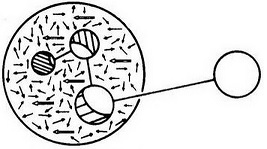
\includegraphics[scale=.6]{a20141010Subration-img001.jpg}
\end{wrapfigure} 

Their action is illustrated in the diagram on the right, taken from \emph{Gnosis} by \textbf{Boris Mouravieff}. The A influences come from every direction and their net, or vector sum, is zero. Although we may be temporarily in a region of similar A influences, overall, they subrate each other and lead nowhere.

The B influences (represented by the thicker arrows), on the other hand, are consistent and flow in the same direction. These are our encounters with the Real. Hence, the next step in esoteric training is to be vigilant in watching the thoughts that we entertain in our mind. We learn to discard the A influences, while allowing in the B influences.

\paragraph{Science of Being}

\begin{wrapfigure}{rt}{0.35\textwidth}
 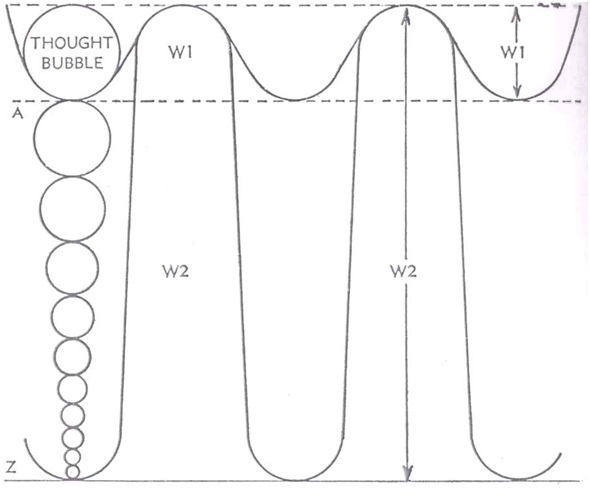
\includegraphics[scale=.35]{a20141010Subration-img002.jpg}
\end{wrapfigure} 

In the same box, I found a yellowing copy of \emph{The Science of Being and the Art of Living}, by \textbf{Maharishi Mahesh Yogi}. Published around the same time as the Deutsch book, it was my initial exposure to Vedantic teachings. Although he was non-traditional in important respects (which we can't get into just now), he was nevertheless well versed in Vedantic doctrines. Since he did propose a path of self-development while being active in the world, he is of a certain interest. In particular, I want to point to a diagram that may help in the process of moving from ordinary to real existents, and then to reality itself.

The goal of vigilance is to improve the quality of thoughts. The Maharishi writes:

\begin{quotex}
The art of thinking should mean that the manner of thinking is such that the least amount of mental energy is consumed … the thought should not only be powerful but it should be right as well. The art of thinking also means that no useless or wrong thought should occupy the mind. 

\end{quotex}
In esoteric training, we learn to observe thoughts. Ordinarily, we become aware of a thought only when it has become fully formed. At that point, further thoughts arise and start linking with each other. At that point we tend to lose full consciousness and become “lost in thought”.

However, by remaining conscious, we may be able to discern the thought in its formation process. This is like bubbles arising; awareness will keep the thought from fully arising. By going into deeper levels of being, we may be able to move beyond the thought into nondual awareness.


\hfill

\flrightit{Posted on 2014-10-10 by Cologero }

\begin{center}* * *\end{center}

\begin{footnotesize}\begin{sffamily}

\texttt{David on 2014-10-21 at 00:46 said: }

Greetings Colgero. A question regarding nonbeing. Could you develop more around it ? My understanding of it was mostly based on Eckhart works, and I was under the impression that for him Non-Being was at the center of creation, from which Being sprung forth and was unknowable. 

The diagram with the arrows is quite simple, yet very effective. I will have to meditate on that. 

Thank you.


\hfill

\texttt{Cologero on 2014-10-22 at 00:37 said: }

Synchronistically, David, a post on that topic has been planned in regards to the Ray of Creation or Great Chain of Being. Your description from Eckhart sounds compatible with what Guenon writes in the Multiple States of Being.


\end{sffamily}\end{footnotesize}


\chapter{Metaphysics of Nonbeing}
\section{Nature Abhors a Vacuum}

In \emph{The Multiple States of Being}, \textbf{Rene Guenon} describes the concept of the Infinite, Being, the World, among other ideas. The following definitions are taken from this work.

\begin{description}
\item[Infinite ]

All possibilities 

\item[Non-Being ]

Possibilities of non-manifestation and possibilities of non-manifestation not manifested 

\item[Being ]

Manifested possibilities 

\item[World ]

A domain formed by a certain ensemble of compossibilities which are realized in manifestation. 

\item[Void ]

Absence of any formal qualities or anything to do with any mode of manifestation 

\end{description}
He points out that the \textbf{Void} has no possibility to be manifested in any world, by its very definition. For those who think that metaphysics has no practical application, this idea demonstrates its fruitfulness for our understanding.

First of all, in the purely physical sense, a Vacuum cannot actually exist. Even is you deny the existence of the Ether, which physics has not really completely ruled out, there is more than nothingness going on in what we call a vacuum.

But more important for our purposes, the non-manifestation of the Void tells us something about the cosmic environment. There can be no gaps in the psychic and physical processes; that it, there is necessarily a continuity synchronically and diachronically. Another way to say it is that everything is in relationship to everything else. Guenon writes:

\begin{quotex}
The cosmic environment can only be conceived of as a whole of which each part is linked to every other part without any break in continuity. To try to conceive of it otherwise would be to assume the existence of a void, but this is not a possibility of manifestation and can have no place in the Cosmos. 

\end{quotex}
This, we have been at pains to point out the relationships between civilizations, traditions, and the transitions from age to age of the cosmic cycle. So what we experience now is in in continuity both with the past and also with everything else contemporaneous. The whole weight of the past is with us now. Hence, something, for example a particular tradition, cannot have been lost and then suddenly reappear.



\flrightit{Posted on 2011-02-10 by Cologero }

\section{The Void and the Fullness are Indissolubly Bound}

\begin{quotex}
We never start from the ``many", but from the ``One" in a state of privation which is correlative to the appearance of others around and against it, in order to move to the ``One" in a state of fullness and sufficiency, in which such an appearance is consummated. \flright{\textsc{Julius Evola}}

\end{quotex}
To understand the creation of the world, we need to begin with the concept of privation\footnote{\url{https://www.gornahoor.net/?p=1815}}. ``Privation" is the absence of a given form in something capable of possessing it. As it is a lack, it has no being in itself, yet it is part of experience. Whatever appears to limit me, whatever seems to oppose my Will, reveals an insufficiency in me, that is, a ``privation". Rather than simply representing a lack or insufficiency, a being may embrace privation and deliberately choose to limit itself. \textbf{Boris Mouravieff} writes (\emph{Gnosis}, Vol 1):

\begin{quotex}
Orthodox Tradition teaches that the Universe was created by a \emph{sacrifice of God}. We shall understand this postulate better if we consider that it differentiates between the state of manifested Divinity and that of unmanifested Divinity — which is therefore limitless and free from all conditions. God's sacrifice is \emph{Self-limitation} by manifestation.

\end{quotex}


By this withdrawal, the unmanifested God, the Universal I, creates a space for the Other selves. The relationship is sustained through Love. Mouravieff explains:

\begin{quotex}
To pass or cross from the non-manifested state — a \emph{monopolar} one, concentrated on the unique consciousness of \emph{Self} within which the Divinity remains before the Creation of the World — \emph{the first Idea} which makes the Divinity come out of the state of non-manifestation to become manifest, is necessarily that of the You. This idea, conceived by the divine sacrifice of Self-limitation, has Love, a neutralizing force, or third force. 

\end{quotex}
We can understand this Hermetically. Mouravieff is describing the Macrocosm, which through a consciously willed privation, creates the Other and binds the relationship with love. Man, the microcosm, on the other hand, wills privation, or the Other, spontaneously without conscious choice. Hence, Trials\footnote{\url{https://www.gornahoor.net/?p=1902}} are necessary. In the \textbf{Trial by Suffering}, Man endures the privation in the understanding that it is the product of his own will and consciousness. In the \textbf{Trial by Love}, Man neutralizes the privation by Love, ending the opposition.

In \emph{Meditations on the Tarot}, \textbf{Valentin Tomberg} takes up the same theme. He makes clear that the withdrawal is real, in the sense that Man has a real, noumenal, free existence, not just an apparent, phenomenal one as in pantheistic systems. Tomberg draws on the Cabbalist doctrine of \emph{tsimtsum} to make the point:

\begin{quotex}
The first act of En-Soph, the Infinite Being, is therefore not a step outside but a step inside, a movement of recoil, of falling back upon oneself, of withdrawing into oneself. Instead of emanation we have the opposite, contraction…The first act of all is not an act of revelation but one of limitation. Only in the second act does God send out a ray of His light and begin His revelation, or rather His unfolding as God the Creator, in the primordial space of his own creation. More than that, every new act of emanation and manifestation is preceded by one of concentration and retraction. \flright{\textsc{Gershom Scholem}, \emph{Major Trends in Jewish Mysticism}}

\end{quotex}
Tomberg goes on to clarify:

\begin{quotex}
In other words, in order to create the world ex nihilo, God had first to bring the void itself into existence. He had to withdraw within in order to create a mystical space, a space without his presence — the void. And it is in thinking this thought that we are present at the birth of \emph{freedom}. 

\end{quotex}
A note of clarification is necessary, since Tomberg writes as a cosmologist, not a metaphysician. The void as such can never exist, or be created. Instead, the idea of the void is the ontological space where beings, as possibilities of manifestation, come into existence. The void is freedom, it is the source of creativity. Tomberg summarizes:

\begin{quotex}
The void — the mystical space from which God withdrew himself through his act of tsimtsum — is the place of origin of freedom, i.e., the place of the origin of an \emph{ex-istence} which is absolute potentiality, not in any way determined… These two indestructible elements—the meonic element (``meon"=void) and the pleromic element (plenitude) are indissolubly bound to one another.

\end{quotex}

Originally published on 4 Apr 2011 on medtarot.

\flrightit{Posted on 2023-02-14 by Cologero }

\begin{center}* * *\end{center}

\begin{footnotesize}\begin{sffamily}



\texttt{Santiago on 2023-02-19 at 00:25 said: }

What a remarkable thing, this freedom which God gives us!

Tomberg, elsewhere in this passage, likens the meonic element to the watery void, but the pleromic he associates with a fiery ``spark" of love, given directly by God. Do they really have to be more or less equivalent, as ``indissolubly bound" implies? It almost sounds like the Void and Fullness are the Divinity Itself (I'm tempted to read: God's existence is His essence). But God has to be more than those contingent things, otherwise freedom would not truly be free and love would not be a gift.

It seems like the void is reached through what Tomberg calls ``depersonalization", that is, through the techniques of dispassion taught in the various traditions. Perhaps I'm projecting onto his writings. But the ability to love is what gives us ownership and autonomy of our lives. It has to be better, or in some way ontologically prior.

I hope this comment doesn't sound too pretentious or ignorant. I've been considering this over the past couple days.


\end{sffamily}\end{footnotesize}

\section{The Metaphysics of Nonbeing}

\paragraph{Metaphysics of Being}
\textbf{Thomas Aquinas} developed a comprehensive metaphysics of Being by integrating Philosophy, predominantly via Aristotle. Plato and Plotinus entered into his system indirectly as mediated by Dionysius the Areopagite and Augustine. As such, Scholasticism is consistent with Traditional metaphysics. Of course, by Being, the Scholastics meant much more than what today's naturalists and rationalists accept as existing.

The Medieval conception of being included nonformal as well as formal states of being. From the metaphysical point of view, the nonformal states as understood theologically, may refer to superior states of the being. Even the Russian Orthodox theologian \textbf{Sergius Bulgakov} reached that understanding. In particular, he notes that the guardian angel and the person both share the same essence. In effect, that means that they are different states of the same being.

From the esoteric perspective, then, these states represent the initiatic degrees that correspond to their respective realizations. This was brought out most forcibly in Dante's \emph{Divine Comedy} which used the astrological symbolism of the planetary and stellar spheres to indicate higher and lower states of being that the initiate needs to traverse.

\paragraph{Nonduality}
\textbf{Meister Eckhart} deepened the understanding of the metaphysics of being. Thomism has a limitation that is sometimes misunderstood as a reversion to duality, with a too strong distinction between the natural and the supernatural, between what could be known by reason and what can only be known by faith. Although Scholasticism recognizes a form of knowing — intuition — that is higher than rational or conceptual knowledge, it was Meister Eckhart who developed that notion more fully.

Intuition overcomes the duality of the sensual image and conceptual thought, which are united in spiritual seeing that unites the two. Moreover, some concepts that Thomas had left to faith, can be understood on a deeper level. Specifically, these are the Incarnation and the Trinity. For Eckhart, the Incarnation is much more than an historical event, since it is repeated whenever the Logos is born again in our interiority. By intuition, Eckhart also sees into the Trinity. Since we have recently discussed these ideas, they need not be repeated here.

\paragraph{Nonbeing}
In \emph{The Multiple States of Being}, \textbf{Rene Guenon} points out that a complete metaphysic needs to include Nonbeing as well as Being, as the latter arises from the former. He points out that the West has failed to develop that notion very well. Guenon does mention the notion of the Abyss in Alexandrian Gnosticism as referring to an aspect of Nonbeing.

Independently, \textbf{Nicolas Berdyaev} in Boehme: Unground and Freedom notes that:

\begin{quotex}
Boehme was perhaps the first in the history of human thought to have seen, that at the basis of being and prior to being lies a groundless freedom. 

\end{quotex}
Perhaps, assuming Guenon is correct, \textbf{Jacob Boehme} is not the first in the history of human thought, but is at least the first in the history of Western thought to develop a metaphysic of nonbeing. Guenon's presentation of Nonbeing is rather dry and rationalistic while Boehme's comes from a deeper source, a direct intuition of Nonbeing which he sometimes calls the Unground. In the \emph{Mysterium Pansophicum}, he attempts to describe it. (It is impossible to define, since a definition is a limitation.)

\begin{quotex}
The unground is an eternal nothing, but makes an eternal beginning as a craving. For the nothing is a craving after something. But as there is nothing that can give anything, accordingly the craving itself is the giving of it, which yet also is a nothing or a desirous seeking. And that is the eternal origin of Magic, which makes within itself where there is nothing; which makes something out of nothing, and that in itself only, thought this craving is also a nothing, that is, merely a will. It has nothing, and there is nothing that can give it anything; neither has it any place where it can find or repose itself. 

\end{quotex}
Obviously, the unground is nothing, since it is not itself manifested. There are two important points that follow from this.

\begin{itemize}
\item The Unground contains all possibilities, light as well as darkness, good as well as evil, God's wrath as well as God's Love. 
\item Being arises from Nonbeing. A fortiori, there is a “craving” for Being, and thus this can be described as a primal Will. Moreover, since Nonbeing is undetermined, it must be perfectly free. 
\end{itemize}
This is just the surface, as Boehme brings an understanding to many other notions, although this is not the time to discuss them.

\paragraph{Letting Go}
In his commentary on the \emph{Secret of the Golden Flower}, a Chinese alchemical text, \textbf{Carl Jung} writes:

\begin{quotex}
The art of letting things happen, action in nonaction, letting go of oneself, as taught by Master Eckhart, became a key to me with which I was able to open the door to the “Way”. The key is this: we must be able to let things happen in the psyche. For us, this becomes a real art of which few people know anything. Consciousness is forever interfering, helping, correcting, and negating, and never leaving the simple growth of the psychic processes in peace. It would be a simple enough thing to do, if only simplicity were not the most difficult of all things. It consists solely in watching objectively the development of any fragment of fantasy. 

\end{quotex}
Jung is referring the Eckhart's idea of “letting go” or \emph{gelassenheit}. Obviously, this is more like the Hermetic teaching of concentration without effort. Simplicity is the detached awareness of whatever psychic processes may be occurring. This watching often dissipates any interference in the psychic process. This letting go then allows something else, something much deeper, to arise. There is a primal will, different from purposeful and conscious willing, that is in touch with more possibilities. In a phrase reminiscent of Jacob Boehme, Jung explains this idea:

\begin{quotex}
Whether arising from without or within, the new thing came to all those persons from a dark field of possibilities; they accepted it and developed further by means of it. It seemed to me typical that, in some cases, the new thing was found outside themselves, and in others within; or rather, that it grew into some persons from without, and into others from within. But it was never something that came exclusively either from within or from without. If it came from outside the individual, it became an inner experience; if it came from within, it was changed into an outer event. But in no case was it conjured into existence through purpose and conscious willing, but rather seemed to flow out of the stream of time. 

\end{quotex}
The important notion is that a change from within brings the outer event into existence. The art of “letting things happen” in the psyche, or action in nonaction, needs to be developed. Then we may experience synchronicities in our lives, or perhaps better said, “grace”. In other words, the pursuit of the outer needs to yield to an interior transformation. This ties in nicely with what Eckhart writes in Sermon 77 about asking God for gifts:

\begin{quotex}
I say, `God is Love,' because He must love all creatures with His love, whether they know it or not. … I will never pray to God for His gifts, nor will I ever thank Him for His gifts, for if I were worthy to receive His gifts He would have to give them to me whether He would or not. Therefore I will not pray to Him for His gifts, since He must give: but I will surely pray to Him to make me worthy to receive His gifts, and I will thank Him for being such that He has to give. Therefore I say, “God is Love,” for He loves me with the love with which He loves Himself: and if anyone deprived Him of that, they would deprive Him of His entire Godhead. Though it is true that He loves me with His love, yet I cannot become blessed through that: but I would be blessed by loving Him and be blessed in His love. 

\end{quotex}
\paragraph{The Purification of the Will}
That is a very important lesson in how to pray. There is no point to pray to God for his gifts, because he is by nature willing to disperse his gifts freely. Rather, the prayer should be to be made worthy to receive the gifts. (Seek ye first the kingdom of God, and his righteousness; and all these. things shall be added unto you.) Thus, the inner transformation comes first, and only then perhaps the external things and events.

To become worthy means to please God. That is the purification of the will. Failure to achieve that will bring obstacles to life. The introduction to the Mass of the 20th Sunday after Pentecost in the Roman Missal makes this clear:

\begin{quotex}
The Liturgy shows us that our misfortunes are caused by our unfaithfulness in conforming to the will of God. Let us beseech the Lord, through the prayers of Holy Church, to pardon our sins, so that we may serve Him with a quiet and trustful heart, always obeying His precepts. 

\end{quotex}
And from the Introit:

\begin{quotex}
Blessed are the undefiled in the way; who walk in the law of the Lord. 

\end{quotex}
\paragraph{Freedom and License}
To be “undefiled” is to be made worthy. Undefiled = pure, so our previous tasks of the purity of the mind and the purity the will must not be forgotten. The result is to walk in the law of the Lord. For Eckhart, that is not a restriction on freedom as the world wants to believe, but is rather freedom itself. He writes:

\begin{quotex}
For the man who stands in God's will and in God's love it is a joy to do all the good things God wills, and to leave undone all the evil things which are against God. And it is impossible for him to leave a thing undone which God wants to have accomplished. As it would be impossible for one to walk whose legs are bound, so it would be impossible for one to do ill, who is in God's will. 

\end{quotex}
Eckhart is emphatic that this does not mean the license to do anything at all:

\begin{quotex}
Some men say: If I have God and God's freedom, then I can do everything I want. They understand these words amiss. As long as you can do anything which is against God and His commandment, you do not have God's love; you can only deceive the world into the belief that you have it. 

\end{quotex}
This is opposite of the contemporary view that if any action motivated by “love” is thereby legitimate. However, that idea is still focused on the “self”, but the self is precisely that which occludes the Will of God. The attachment to sensory images and intellectual ideas are obstacles to spiritual vision. If redemption is the recovery of the primordial state prior to the Fall, this state can be understood only by a pure mind. \textbf{Wolfgang Smith} elucidates this point:

\begin{quotex}
The Patristic understanding of Paradise is mystical in two respects: first, because it insists that the nature of Paradise exceeds categorically what the “carnal man” — St. Pauls \emph{psychikos anthropos} — is able to comprehend; and secondly, because it claims that the things of Paradise can in fact be “seen” when certain degrees of contemplation have been attained. St. Gregory the Sinaite speaks of this explicitly when he explains “the eight primary visions accompanying the state of perfect prayer when things previously happen are clearly beheld and known by those who have attained by grace complete purity of mind.” 

\end{quotex}
Eckhart knows that teaching also:

\begin{quotex}
Not an already existing life — “being” — is to be understood in the logical sense; but the higher understanding — “seeing” — is itself to become life; the spiritual, that which belongs to the idea, is to be experienced by the seeing man in the same way as the individual human nature experiences ordinary, everyday life. 

\end{quotex}
For that to occur, depth is required, where there is a perfect “morality”, i.e., the Will of God is known. The world lives on the surface: it looks for understanding (i.e., “explanations”) and the satisfaction of desires. There is a fear of “letting go”, for the end of understanding is experienced as darkness. However, God's light shines precisely in that darkness. Eckhart writes:

\begin{quotex}
For everything the understanding can grasp, and everything desire demands, is not God. Where understanding and desire have an end, there it is dark, there does God shine. There that power unfolds in the soul which is wider than the wide heavens. The bliss of the righteous and God's bliss is one bliss; for when God is blissful, the righteous are blissful. 

\end{quotex}


\flrightit{Posted on 2017-11-19 by Cologero }

\begin{center}* * *\end{center}

\begin{footnotesize}\begin{sffamily}



\texttt{jonathansolvie on 2017-11-20 at 10:22 said: }

Great work!

“For Eckhart, the Incarnation is much more than an historical event, since it is repeated whenever the Logos is born again in our interiority.”

This is true with the qualification that the esoteric understanding of the incarnation of the Logos within the initiate by no means dispenses with the objective and macrocosmic significance of the Incanation that took place in the historical Jesus Christ, non-dually uniting time and Eternity, concrete event and universal metaphysical truth and symbolism. While the Logos that incarnates in any initiate of the Greater Mysteries may be principally non-dual with Christ (“I am crucified with Christ, but I live; yet not I, but Christ liveth in me”), the incarnations are are from equal in the persons of Jesus of Nazareth and Meister Eckhart in terms of total manifestation and macrocosmic and eschatological function. Yes, the incarnation of the Logos reflects in the mirrors of many Hearts, but there nevertheless needs be one Incarnation in the unfolding within time of a human world-cycle that is unique, preeminent and unsurpassable, as the highest peak of personal divine manifestation within creation. Therefore the above esoteric interpretation of Incarnation within our own Heart depeens our understanding of the principle of Incarnation, but does not exhaust the esoteric depth of the historical Incarnation, which has a macrocosmic dimension as well, the delving into which would allow us to understand also the literal truth of exoteric dogma regarding the Incarnation as an objective and historical macrocosmic and eschatological event, and yet in more profound hermetic depth.


\hfill

\texttt{jonathansolvie on 2017-11-20 at 15:43 said: }

Some might assume from reading this article that the `Unground' is the Absolute, since Being is said to proceed from it. However, the Absolute Reality, the Gottheit, is not nothingness or non-being as opposed to Being; both of these are `dependently originated' and mutually conditioned. Since non-being stands in relation to Being, it is not undetermined. The very `craving' explained as arising from the Unground testifies to its limitation and its need for Being which stands as its opposite pole. If from one perspective Being arises from the former, both derive their reality from the unconditioned freedom of the Absolute. The undetermined and infinite Reality is beyond both Being and non-being, the manifest and the unmanifest, and the latter is not superior to the former in face of That. 

I just thought this might be worth pointing out for certain readers; I do not mean to correct the author, who undoubtedly knows this better than I.


\hfill

\texttt{Fred on 2017-11-21 at 16:05 said: }

I agree with jonathansolvie.

Possibly the Absolute is even beyond Being and Non-Being, not only beyond all affirmations but also beyond every negation.

There was a time where I tried to study the highest metaphysics, then a monk told me studying the mystics is of no benefit if you are struggling with the purification of beginners. I'm much more comfortable with the daily fights now.

I will keep following this advice until it's time.


\hfill

\texttt{Cologero on 2017-11-21 at 21:18 said: }

Thanks, Fred and jonathansolvie, for making that clarification. Yes, I was unclear about Non-being and the Absolute. Moreover, I had in mind the Absolute as universal Possibility, without explicitly stating so. There is certainly work to do in adequately relating Boehme's insights to traditional metaphysics. This will be an ongoing project.


\hfill

\texttt{Cologero on 2017-11-21 at 21:22 said: }

Yes, jonathansolvie, those are good points. The esoteric is not intended to replace or supersede the exoteric. That is what you may find in certain Gnostic or Theosophical circles which claim to reveal the “true” meaning of the exoteric.


\hfill

\texttt{Caeliger on 2017-11-22 at 03:42 said: }

Non-Being is not merely the `void'. which follows the primordial `contraction' or expiration of God (needless to say, this must happen `before the foundation of the world’), but we could say that the void is one of its `aspects'. one which will explore the possibilities of the One and the many. 

It could certainly be taken in a limiting sense as `that which is opposed to Being'. in which case it is indeed necessary to conceive a yet higher priciple which is truly infinite.


\hfill

\texttt{Arthur Konrad on 2017-11-22 at 11:50 said: }

“Some men say: If I have God and God's freedom, then I can do everything I want. They understand these words amiss. As long as you can do anything which is against God and His commandment, you do not have God's love; you can only deceive the world into the belief that you have it. ”

This is valid only if interpreted on non-moralistic grounds. Otherwise it makes no sense. There is either inner freedom and hence inner commandment, or you do not posses inner will at all. Discovering inner will absolutely does not equate discovering any commandments not one's own, since one's fate is then already perfectly clear and resolved (hence utter futility in attempting to draw parallel between inner will and religious law). Ekchart has deployed a rather worn out linguistic device here to draw a parallel between apparently religious commandment and an inner will, which demands an esoteric interpretation to overcome it's obstacles.


\hfill


\hfill

\texttt{Numen on 2017-11-23 at 01:24 said: }

jonathansolvie's clarification is excellent and succinct.

S.H. Nasr once explained in a presentation that the basis of the theme of the void in Islamic art stems from the understanding that “if the world is everything, then God is nothing; If God is everything, then the world is nothing.” In a sense, our understanding of God has to oscillates between the two (Being and Non-being); the Non-being of God has to be a part of the transcendent principle, otherwise God is seen just merely as Being, part of the manifestation itself. Or, as Eckhart put it, God is “Being above Being and superessential Negation.”

Dante's intuition is nicely simplified when he wrote: “as certain things are affirmed to exist which our intellect cannot perceive (namely God, eternity, and primal matter), things which most certainly are known to exist and are with full faith believed to exist. But given the nature of their essence we cannot understand them: only by negative reasoning can we approach an understanding of these things, and not otherwise.”


\end{sffamily}\end{footnotesize}

\section{Logos and Chaos}

The idea of Chaos was known to the early Greeks. The poet \textbf{Hesiod} wrote:

\begin{quotex}
First of all, Chaos came into being; then Earth with her broad breast, for all things a seat secure forever. 

\end{quotex}
\textbf{F. M. Cornford} explains that Chaos is not `formless disorder'. as we conceive it today, but rather the `yawning gap' between earth and heaven. \textbf{Euripides} wrote: `Heaven and Earth were once one form.' In the Rig Veda, Varuna `held asunder spacious Earth and Heaven.' For the ancient Egyptians, \emph{Shu} separates \emph{Nut} (sky) from \emph{Seb} (earth). Of course, in China it was taught that from the Tao came the duality of Yin and Yang, Earth and Heaven.

In the ancient sense, Chaos does not represent the destruction of the ordered physical world, but rather the unmanifested Void that is the principle of heaven and earth, male and female. So behind the physical world, there is a principle that represents the unity of Being. For \textbf{Heraclitus}, there is one Logos, one reason for everything, throughout “the one cosmos which is the same for all.”

\textbf{Rene Guenon}'s criticism of Western theology is that it stops at the consideration of Being alone, and does not penetrate beyond Being. This is true to the extent that God is understood as Being, which is true from the point of view of manifestation. Nevertheless, some figures such as \textbf{Meister Eckhart} and \textbf{Jacob Boehme} have recognized the “God beyond God” or the Urgrund (Void) ontologically prior to Being. In the East, there is the understanding of the difference between the essence and energies of God. In a metaphysical sense, the West can perhaps be accused of a forgetfulness of Non-being rather than the forgetfulness of Being.

Guenon identifies the Divine Intellect as the `location' of the eternal ideas. In his conception, the theologian only recognizes the possibilities of manifestation, whereas the metaphysician also recognizes the possibilities of non-manifestation. Guenon identifies the Divine Intellect as the Logos (or Word), which is the principle of manifestation since all things are created from it. Hence, at the metaphysical level Logos is the same as Chaos, as the unifying principle of manifestation. The Logos can also be identified with the Tao, as Tao is used in Chinese translations of the Bible for the Logos.

In Mathematics, Chaoas Theory\footnote{\url{https://en.wikipedia.org/wiki/Chaos_theory}} demonstrates that there can be a hidden order behind seemingly chaotic systems.

\begin{quotex}
Chaos theory states that within the apparent randomness of chaotic complex systems, there are underlying patterns, interconnectedness, constant feedback loops, repetition, self-similarity, fractals, and self-organization. 

\end{quotex}
Thus, there is no opposition — and there cannot be — between Logos and Chaos at the metaphysical or transcendental level. There the battle has already been won. Hence, the battle is fought on the \emph{psychic} and \emph{hylic} levels, that is, between \emph{cosmos} and \emph{chaos}, which can be understood as `formless disorder' only at this level\footnote{References:

[1] From Religion to Philosophy, F. M. Cornford

[2] Miscellanea, Rene Guenon}.

This will be explored in the “Conditions of Corporeal Manifestation”.


\flrightit{Posted on 2012-09-19 by Cologero }

\begin{center}* * *\end{center}

\begin{footnotesize}\begin{sffamily}


\texttt{Cassiodorus on 2012-09-20 at 01:19 said: }

Cologero,

I recently discovered this site and I've been devouring the many interesting and insightful posts . There is something that I am somewhat puzzled about. Being that Rene Guenon has such prominent role here, why is there such a dearth of treatment of Frithjof Schuon and others of the Traditionalist school?


\hfill

\texttt{Andrew on 2012-09-20 at 15:59 said: }

This actually answers (at least in part) a question I had asked about Buddhism and Tradition. In Buddhism the condition for a thing is its principle.

If the Void is the Principle of Manifestation, then Form is Emptiness, Emptiness is Form. Another name for Shunyata (Voidness) is Dharmadhatu (which I translate as “World of the Word”). Also, the Buddha said, “He who sees Dharma sees Me; He who sees Me sees Dharma”.


\hfill

\texttt{Logres on 2012-09-20 at 21:57 said: }

Cologero has stated that he doesn't post on Schuon because there are (in his judgement) many well done sites on such already. At least this was his answer if my memory serves, last time it was brought up.


\hfill

\texttt{Cassiodorus on 2012-09-20 at 22:49 said: }

Cologero or Logres,

I'm an ex- postmodern agnostic that discovered the teachings of Tradition and the Perennial Philosophy several years ago. Since then, the focus of my studies has centered on Catholic Christianity, resulting largely from my increasing acquaintance with the Church fathers and, most importantly, with the Angelic Doctor, Thomas Aquinas. Interestingly, I've noticed that most traditional Christians are hostile to the Primordial Tradition, quick to make the charge of pantheism, monism, or even gnosticism. For most Thomists that I've spoken to, the Perennial Philosophy is often rejected on the grounds of being a modern variant of “eastern mysticism” and that Tradition is antithetical to monotheism by blurring the line that separates God and man. Plainly stated, do you think there is a problem in reconciling the classical theistic traditions of the West with nondualism and the doctrine of the Self?


\hfill

\texttt{Cologero on 2012-09-20 at 23:42 said: }

Cassiodorus, rather than ask why we don't do something–a negative, the better question is to understand our purpose. Primarily, it is to determine how Tradition can be recovered in the West. Coincidentally–if you believe in coincidences–your namesake serves as a suitable model. The real Cassiodorus was able–in his own mind–to integrate the Ancient with the Medieval, the Latin West with the Greek East, the Roman with the Germanic.

We agree with Guenon that Medieval Europe had more in common with the civilizations of the East than with the Modern West. Even “traditional” Catholics go back only to the Council of Trent and are thus still far from the worldview of the Medievals. Following various suggestions by Guenon, we have pointed out the commonality of the doctrines of Thomas with other Traditions. Thomism today is reduced to a “philosophy”, one among other competing systems. However, it must be understood as a metaphysics, which is known experientially, not just rationally; it is totalitarian, demanding one's total adherence.

Thomism will be deepened by the encounter with Tradition. Some can't see it; others do. The charges of pantheism or gnosticism arise because of a misunderstanding of Being or an ignorance of Christian gnosis.

When you can make a certain shift in consciousness, many seemingly insoluble puzzles are resolved.


\hfill

\texttt{Cassiodorus on 2012-09-21 at 01:15 said: }

Cologero,

Many thanks for your thoughtful response. “Thomism will be deepened by the encounter with Tradition. Some can't see it; others do.” This comment reminded of something that Ananda Coomaraswamy said in “Vedanta and the Western Tradition”,

To say that “I am a pantheist” is merely to confess that “I am not a metaphysician,” just as to say that “two and two make five” would be to confess that “I am not a mathematician.”

Nevertheless, on the subject of Christian gnosis, I've been told by both Catholics and Orthodox that there is a fundamental difference between Christian divinization, theosis, and the Indian Supreme Identity, moksha. Furthermore, it is said, the Perennial Philosophy that Agostino Steuco and Leibniz refer to cannot be expanded to encompass the traditions of the East because participation in the Divine and identification with the Divine represent two incompatible ontologies. 

Would you say that apophatic theology and pure metaphysics are essentially the same thing?

Best Regards,

Cassiodorus


\hfill

\texttt{Cologero on 2012-09-21 at 08:05 said: }

Cassiodorus, find the man who has experienced both “participation” in the divine and moksha; I'm sure he could explain the differences to us. Otherwise, it is idle chit chat. This is a journey every man must make for himself and he can't rest content just reading someone else's postcards.


\hfill

\texttt{Cassiodorus on 2012-09-21 at 10:13 said: }

I believe I see your point.


\hfill

\texttt{Michael on 2012-09-21 at 20:32 said: }

Cologero, so how does one go about experiencing Aquinas and not just absorbing his writings rationally? Sorry for the ignorant questions.


\hfill

\texttt{Cologero on 2012-09-22 at 10:08 said: }

It is not an ignorant question, but the only question worth asking. Check out Letters of AKC\footnote{\url{http://akc.satishankar.com/2012/09/selected-letters-of-ak-coomaraswamy.html}} and read the intro to the first volume. Then bring up the topic again.


\hfill

\texttt{Cologero on 2022-02-12 at 08:04 said: }

Although too much Wittgenstein is risky, a small dose may be helpful:

“Whereof one cannot speak, thereof one must be silent.”

Otherwise, one is just engaging in a language game, trying to make various propositions compatible with each other. Well, the world is not a proposition nor a riddle to be solved.

“Thinking”, as important and as pleasant as it is, is nevertheless a low stage of development, actually only at stage three of Augustine's seven stages of the ascent to God\footnote{\url{https://www.gornahoor.net/?p=10801}}.


\end{sffamily}\end{footnotesize}


\chapter{Epistemology}
\section{Esoteric Epistemology}

\begin{quotex}
For the whole human being is at one and the same time a mystic, a gnostic, a magician and a philosopher, i.e., he is religious, contemplative, artistic and intelligent. \flright{\textsc{Valentin Tomberg}, \emph{Meditations on the Tarot}}

\end{quotex}
In the secular world, this is the epistemological question:

\begin{quotex}
What do you know and when did you know it? 

\end{quotex}
However, this misses the more important question:

\begin{quotex}
How do you know and what do you know when you know it?

\end{quotex}
In metaphysics, epistemology follow ontology, i.e., knowledge follows the sequence of manifestation, like this:

\begin{enumerate}
\item \textbf{Mystical experience}: The pure act of knowledge of the Self 
\item \textbf{Gnosis}: The intuitive knowledge of the Divine Intellect 
\item \textbf{Magic}: The expression of that knowledge in representations and imagination, whose source is the Manas. 
\item \textbf{Philosophy}: The above three states expressed in language, which is proper to the human state. 
\end{enumerate}
Tomberg describes the stages in more detail:

\begin{quotex}
This transformation of mystical experience into knowledge takes place in stages. The first is the pure reflection or a kind of imaginative repetition of the experience. The second stage is its entrance into memory. The third stage is its assimilation in thought and feeling, in a manner where it becomes a “message” or inner word. The fourth stage, lastly, is reached when it becomes a communicable symbol or “writing”, or “book”—i.e., when it is formulated. \flright{\textsc{Valentin Tomberg}}

\end{quotex}
\paragraph{Short Circuits}
There can be deformations of this transformation, such as:

\begin{enumerate}
\item Remaining stuck in mystical experience, just for the pleasure of it. 
\item Gnosis detached from revelation and tradition lacks any foundation. Gnosis is mysticism that has become conscious of itself. 
\item Imagination without gnosis becomes pure fantasy 
\item Philosophy becomes pure speculation, and lacks truth 
\end{enumerate}
\paragraph{Metaphysical and Profane Knowledge}
IT is a misconception to assume that the method of metaphysical knowledge is identical to our knowledge of the corporeal world. These are the main differences between the two ways of knowing.

\begin{itemize}
\item Metaphysical knowledge is based on the faculty of intuition, which is a direct experience of the real and permits contact between our consciousness and the world of pure mystical experience. Profane knowledge is based on the inferior faculty of the rational mind. 
\item Metaphysical knowledge is deductive, that is, it begins with higher principles and applies them to particular situations. Profane knowledge is inductive, or better said, abductive. 
\item Metaphysical knowledge depends on the level of being of the knower. Hence, spiritual practices such as concentration, meditation, prayer, purification of the soul, and so on, are necessary. Profane knowledge, on the other hand, does not depend on the personal character of the knower. 
\item Metaphysics is known with apodictic certainty and profane knowledge is uncertain and subject to revision. 
\end{itemize}
\paragraph{The Temptation of Philosophy}
There is a certain blindness in the human being. Those with the intellectual talent often believe that the mere accumulation of books will somehow bring them to gnosis and mystical experience. As we see above, the book is the last stage of the process. Not all mystics and gnostics have the ability to write good books, and certainly fewer can write good poetry.

No matter how many times they hear or read that self-knowledge is more important than book knowledge, it fails to make any impact. You know the type; try to avoid it.

Whenever you think you may have some great idea, don't forget that over the centuries people more intelligent, more educated, and more insightful than you have thought about those issues that so interest you. Turn to the classic authors first, whose thought has endured over the centuries; prefer them to more recent authors.

\paragraph{The Temptation of Science}
\begin{quotex}
Science begins with facts (the “characters” of the book of Nature) and ascends from facts to laws and from laws to principles. Gnosis is the reflection of that which is above; science, in contrast, is the interpretation of that which is below. The last stage of gnosis is the world of facts, where it becomes fact itself, i.e., it becomes “book”; the first stage of science is the world of facts which it “reads”, in order to arrive at laws and principles.

\end{quotex}
There are two ways to understand the Fall of Man:

\begin{itemize}
\item From the moral point of view, Adam and Eve disobeyed God's command and were punished for it. 
\item From the gnosis point of view, Adam and Eve replaced the intuitive knowledge of the Good with the empirical knowledge of good and evil. This had enormous consequences. 
\end{itemize}
The age-old question is, “Is something good because God commanded it, or did God command it because it was good?”

The moral view is based on the first premise and the gnosis view on the second premise.

Science is based on knowledge that begins with, and is restricted to, the sense. It can only produce falsifiable predictions, not certain knowledge.



\flrightit{Posted on 2021-06-27 by Cologero }

\section{The Metaphysics of Knowing}

\paragraph{Sense Knowledge}
Sense knowledge is known through the senses and mediated by thought. There are three inner aspects involved in knowing.

\begin{itemize}
\item \textbf{Sensation}. The senses apprehend an object 
\item \textbf{Imagination}. The mind forms and image of the object 
\item \textbf{Intellect}. The intellect knows what the object is 
\end{itemize}
What the intellect knows is the form or essence of the object. In that case, the knower \emph{is} the thing, since its essence exists in his mind. However, he is \emph{not} the thing in terms of its existence in manifestation. This is the principle that knowledge is being.

A consequence is that deeper understandings are possible. For example, some people are attuned to animals. They are grasping more of the essence than most people. Others, like Padre Pio, can read men's souls.

\paragraph{Abstract Knowledge}
Beyond sense knowledge, there is knowledge that derives from abstracting from the world of sense. These are necessary and universal principles, which are independent of all particular facts in space and time. In other words, they are forms of thought. There are three levels of abstraction:

\begin{itemize}
\item \textbf{Natural Science}. This is the science of the inner universal nature of mineral, plans, and animals, apart from any particular thing. 
\item \textbf{Mathematics}. This includes arithmetic, the science of number, and geometry, the science of shapes. Again, these are abstracted from any sense qualities. 
\item \textbf{Metaphysics}. This is the science of Being in which the intellect recognizes the characteristics of being as such. We previously outlined the main principles of this science. 
\end{itemize}
These abstract sciences demonstrate the immateriality of the soul. Since its knowledge is beyond time, and knowledge is being, the intellectual soul is likewise beyond time.

\paragraph{Analogical Knowledge}
Since the natural man knows through sense, imagination, and thought, his understanding of spiritual things also begins in the senses, or imagination. That is why spiritual things are explained in terms of images, art, or symbols. That is a way to get to the thought about such things.

The principle of analogy then is that the intellect knows God and spiritual beings by analogy with the sense world. That is, the knowledge of spiritual things is mediated by the imagination and thought.

However, those who do not understand this principle, are able to conceive the spiritual world only in sensual imagery. This leads to misconceptions and distortions.

Therefore, it is necessary to grasp this principle. In Hermetism, this is expressed in the formula, “As above, so below.”\textbf{ Valentin Tomberg} explains this principle:

\begin{quotex}
Analogy is the first and principal method whose use facilitates the advance of knowledge. It is the first conclusion drawn from the tenet of universal unity. Since at the root of the diversity of phenomena their unity is found in such a way that they are at one and the same time different and one, they are neither identical nor heterogeneous but are analogous insofar as they manifest their essential kinship. 

\end{quotex}
Both Valentin Tomberg and Rene Guenon offer extensive discussions of how to understand metaphysical and religious symbolism. They are worth the study.

\paragraph{Intuitive Knowledge}
A direct, intuitive knowledge (not mediated by symbols or thought) is possible beyond the natural state. This is the way angelic intelligences know. \textbf{Fr Reginald Garrigou-Lagrange} explains knowledge in the postmortem state:

\begin{quotex}
The separated [i.e., postmortem] soul knows itself directly, without medium. … By this immediate self-knowledge, it sees with perfect evidence its own native spirituality, its immortality, its freedom. … It knows God, no longer in the sense world as mirror, but as mirrored in its own spiritual essence. It sees with transcendent evidence the solution of the great philosophic problems, and the absurdity of materialism, determinism, and pantheism. [postmortem] souls have knowledge of one another and the angels. 

\end{quotex}
Clearly, that explanation leaves out of consideration the possibility of achieving such states before physical death. Of course, the whole point of the spiritual path of theosis is indeed to achieve such states. We have the testimony of those who have achieved them and we have the metaphysical understanding that shows such states are possible while alive.

Knowing in this way is the way that angels know\footnote{\url{https://www.gornahoor.net/?p=2995}}. Angelic intelligences can also be understood as higher states of being, i.e., beyond the natural man.



\flrightit{Posted on 2014-09-29 by Cologero }

\section{Self-Realization through Knowledge}

According to \textbf{Fr Reginald Garrigou-Lagrange}, there are three orders of knowledge: human, angelic, and divine. They each have their proper object of knowledge:

\begin{itemize}
\item \textbf{Human}: Sense objects. 
\item \textbf{Angelic}: His own angelic essence 
\item \textbf{Divine}: His own divine essence 
\end{itemize}
Note the lack of symmetry in the object of human knowledge. That is because the natural man is a determinate, material being, unlike angels and God. The type of knowledge proper to man is subject-object and discursive, whereas spiritual knowledge is intuitive and direct.

To restore the symmetry, we can consider the possibility that the proper object of man's knowledge is analogously his own essence. That necessitates the transcendence of the natural human state. Actually, this is the only true knowledge, since our knowledge of sensual things is more properly classified as opinion. \textbf{Rene Guenon} asserts:

\begin{quotex}
The being assimilates more or less completely everything of which it is conscious; indeed, there is no true knowledge in any domain whatsoever, other than that which enables us to penetrate into the intimate nature of things, and the degrees of knowledge consist precisely in the measure to which this penetration is more or less profound and results in a more or less complete assimilation. In other words, the only genuine knowledge is that which implies an identification of the subject with the object.

\end{quotex}
Thus, to understand one's own essence, one must become more and more conscious of himself. This knowledge is not discursive, but rather intuitive and non-dual. Keeping in mind the principle that “knowing is being”, this means that the more we know (in this sense), the more being we have. This knowing is identical to achieving higher states.

It is helpful, therefore, to understand the sense in which angels know in order to achieve such states. Furthermore, we are commanded to “know God”. Clearly, then, this means to achieve a certain state of being, which is the idea of \emph{theosis}.

\paragraph{Angelic Knowledge}
Angels do not acquire knowledge through sense objects. They know ideas, which are in the divine mind, directly. This knowledge is both universal and concrete; that is, it is knowledge both of essence and existence. In Guenonian terms, the former is the knowledge of possibilities and the latter of those possibilities as manifested. However, their knowledge is not co-extensive with the infinity of all possibilities.

The angelic ideas represent a region of intelligible reality and each angel has his own domain. The angels themselves form a hierarchy; since this represents a difference in level of being, there must likewise be a difference in level of knowledge. Fr Garrigou-Lagrange explains:

\begin{quotex}
The higher the angel, the stronger is his intelligence and the fewer are his ideas, since they are more rich and universal. Thus, with ever fewer ideas, the higher angels command immense regions of reality, which the lower angels cannot attain with such eminent simplicity. A human parallel is the sage who, in a few simple principles, grasps an entire branch of knowledge.

\end{quotex}
We noted something similar to this previously when discussing abstract knowledge. By knowing certain mathematical or metaphysical principles, the expanse of knowledge just opens up. For the angels, their domains over human existence become increasingly more universal. There are guardian angels or daemons for the individual; then there are higher angles that represent nations, and so on.

\paragraph{Classical Theism}
Classical theism\footnote{\url{http://edwardfeser.blogspot.com/2010/09/classical-theism.html}} is the term used by philosophers to represent our conception of God. The downside of this is that it may seem that it is just one possible conception among others, which are then debatable. However, the more correct understanding is that classical theism is the correct conception and all others are simply misconceptions. (For more details from a philosopher's viewpoint, please visit the link provided.)

While it can be difficult to grasp, it is worth the effort since it reveals many problems in regard to God to be pseudo-problems. The common mind still tends to conceive of God as a Zeus-like figure, that is, a very powerful being, involved in time, interfering in the affairs of men, and so on. Even many philosophers and theologians have but a more sophisticated view of Zeus.

Fundamentally, God is Being itself. As Guenon points out, Being is a possibility of non-manifestation, hence God cannot exist as a being among other beings; furthermore, the corollary is that God is non-material. Being is the cause of Existence, by making the potential actual.

God's knowledge is not different from his being (knowing=being). He knows all possibilities, directly, as they subsist in the divine mind. In particular, God's knowledge cannot take the form, “God knows all true propositions”, as I read on a blog a short while ago.

There is a logical consequence of this, that is seldom brought out. As we pointed out last time, when I know a squirrel, for example, I am that squirrel insofar as the idea subsists in my mind. Since the idea of the squirrel, both as an abstract and universal idea, as well as each particular squirrel, we can assert that God is likewise a squirrel, a tree, and so on for everything, insofar as he knows himself. This is not quite pantheism, since we can't go in the other direction and say, for example, that the squirrel is God.

Higher than all the angels, God knows the entire world, as Guenon defines the world as:

\begin{quotex}
the entire domain formed by a certain ensemble of compossibles realized in manifestation; these compossibles must be the totality of possibles that satisfy certain conditions characterizing and precisely defining that world

\end{quotex}
He also knows the world and its future because He wills it.

\paragraph{Consciousness and Knowledge}
God is conscious only analogously to the way man is conscious. Guenon explains that total truth must be coextensive with Being and universal Possibility, while consciousness is a human state. This precludes the idea of God having intentional consciousness, that is, the duality of a subject knowing an object.

In his best book, \emph{Answer to Job}, \textbf{Carl Jung} has an interesting speculation that God is unconscious, which is true from Jung's psychological point of view, and that man is God's consciousness. While Jung tries to describe this psychologically and phenomenologically, there is a more metaphysical interpretation. God does not look out on the world, Zeus-like, from on high; rather, he knows the world, as defined above, in his own mind.

Now, man knows sense objects. Specifically, he not only knows the idea of a tree, he also senses the tree: its color, scent, the rustling of the branches in the wind, etc. God has no physical senses. However, he has a perfect knowledge of man as manifested, hence he knows the tree in the same way the man does. God is psychically unconscious in man. Jung writes:

\begin{quotex}
It is only through the psyche that we can establish that God acts upon us, but we are unable to distinguish whether these actions emanate from God or from the unconscious.

\end{quotex}
This means that we need to differentiate between the influences that impinge on our consciousness: is their source worldly or transcendent? Jung says that through the Holy Spirit, the divine child, or one's real Self, is born in consciousness. God then becomes conscious in man as man becomes conscious of God.

This is self-realization through knowledge.



\flrightit{Posted on 2014-10-01 by Cologero}

\begin{center}* * *\end{center}

\begin{footnotesize}\begin{sffamily}

\texttt{Matt on 2014-10-04 at 12:06 said: }

There was a lot to unpack from this post (which was very good by the way), and so I thought it was best to do a number of re-readings of it before making my comment.

My comment is really just about a question of clarification with respect to the last part of the post on the Answer to Job and God's relation with man. Would God becoming conscious in man be compatible with the principle of God as pure act? It seems that God becoming conscious implies a potential that is yet actualized. I wish I had a copy of Jung's book at hand so I can read it in light of your post.

\hfill

\texttt{Cologero on 2014-10-05 at 17:39 said: }

Nice catch, Matt, but the problem is just that I may have expressed it poorly. Jung does use that type of language, presumably figuratively. Language is simply insufficient. Jung's point is that the consciousness of God is lacking, but man can become more conscious of God. If God knows every person, then his becoming conscious of God is God “becoming” conscious through the person. The “becoming conscious” is a possibility of manifestation, which God knows eternally, so it is not a question of becoming from His point of view, but it is from the person's. This is not a dogma, but it is worth pondering.

\hfill

\texttt{Cologero on 2014-10-07 at 23:40 said: }

“We are not to call any man a real philosopher who is a friend of wisdom for profit, as are lawyers, physicians, and almost all the clergy, who do not study in order to know, but in order to get money or office; and if anyone would give them that which it is their purpose to acquire, they would linger over their study no longer.”

“Beyond the delightful and the useful, there is a love for wisdom for its own sake; wisdom alone is worthy of man. And just as love between men is genuine when each loves the other without reserve, so the true philosopher embraces wisdom in her totality, and wisdom in her totality opens herself to the whole man.”

\flright{\textsc{Dante}}

\hfill

\end{sffamily}\end{footnotesize}

\input{201808_30Losing One’s Head}
\section{The Knower and the Known}


One of the fundamental differences between the Traditional and the modern worldviews regards the nature of knowing. For the modern mind, knowing depends on the thing known and the knower himself is passive. As far back as the Stoics, the analogy used was that of wax taking on the design of a seal; thus, the sense impressions in the mind are the effect of an external object. The moderns took this up again, although it then led to Kantian skepticism since there is no way to be sure the sense impression really matches the external object. On the other hand, those of a scientific bent totally ignored Kant and continued on their quest; this has consequences for the search for artificial intelligence and the Golem.

\begin{wrapfigure}{rt}{0.35\textwidth}
 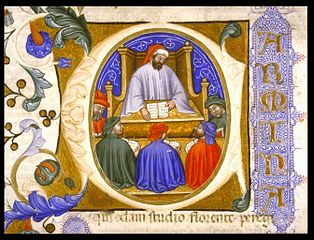
\includegraphics[scale=.5]{a20121023TheKnowerandtheKnown-img001.jpg}  
\end{wrapfigure}

In his Consolations of Philosophy, \textbf{Boethius} addresses the topic and rejects it:

\begin{quotex}
People think that the totality of their knowledge depends on the nature and capacity to be known of the objects of knowledge. But this is all wrong. \emph{Everything that is known is comprehended not according to its own nature, but according to the ability to know of those who do the knowing}. [my emphasis]

\end{quotex}
This needs to be pondered. It means that knowing is not an automatic process and that the object of knowledge does not reveal itself indiscriminately. For example, academics study Tradition as a set of texts that have appeared historically. The academic, then, believes that his impressions represent the truth of Tradition, and all he needs do is to catalog the texts and relate them, temporally or spatially.

But this is all wrong. Only the man who has prepared himself, who has developed within himself the ability to know, only he can understand Tradition. Boethius summarizes the stages of knowledge in the following schema; note, especially, how they relate to \textbf{Dante}'s four levels of understanding an esoteric text. Nothing in Tradition is arbitrary.

\begin{table}[h]\scriptsize
\begin{tabular}{cccc}\toprule 
Stage of knowledge &
Description &
Applies to &
Level of Interpretation\\\midrule
Sense Impression &
The senses examine shape as constituted in matter. &
Lower animals, plants &
Literal\\\midrule
Imagination &
Considers the shape apart from matter &
Higher animals &
Allegorical\\\midrule
Reason &
Transcends the imagination and reflects upon the species inherent in individual instances &
Man &
Moral\\\midrule
Intuition or Intelligence &
Passes beyond the sphere of the universe to behold the simple form itself with the pure vision of the mind. &
Divinity (God, angels, higher states of consciousness) &
Anagogical\\\bottomrule
\end{tabular}
\end{table}
Boethius elaborates:

\begin{quotex}
The point of greatest importance here is this: the superior manner of knowledge includes the inferior, but it is quite impossible for the inferior to rise to the superior. The senses cannot perceive anything beyond matter; imagination does not consider universal species; and reason does not comprehend simple form … [the Intellect] knows reason's knowledge of universals, imagination's knowledge of shape, and the sense's knowledge of matter without using reason, imagination, or the senses, but by the single glance of the mind according to the form.

\end{quotex}
Boethius makes clear that this is an active process:

\begin{quotex}
In perceiving corporeal phenomena the mind is not passively affected, but judges of its own power the experience subjected to the body.

\end{quotex}
This “power”, then, can be developed further and Boethius urges us on:

\begin{quotex}
Let us, then, if we can, raise ourselves up to the heights of that supreme intelligence. There reason will be able to see that which it cannot see by itself—it will be able to see how that which has no certain occurrence may be seen by a certain and fixed foreknowledge, \emph{a knowledge that is not opinion, but the boundless immediacy of the highest form of knowing}.

\end{quotex}
\paragraph{Golems and Artificial Intelligence}
The whole premise of the development of artificial intelligence is based on the passive reception of sense impressions. Since a computer can have no conception of the form of a cube, simple tasks, such as recognizing a box, are very difficult. Through sheer computational power, computers are, and will be, able to simulate intelligence, but not have intelligence in any real sense. Legends of golems and homunculi recognized this. The golem could not be merely a being or mechanism of matter; somehow it would have to be animated. In other legends, higher beings were invoked to animate a statue or a doll. But no one thought mere matter could display intelligence.


\hfill

I'm using the translation by V. E. Watts, published by Penguin Classics



\flrightit{Posted on 2012-10-23 by Cologero }

\begin{center}* * *\end{center}

\begin{footnotesize}\begin{sffamily}



\texttt{Logres on 2012-10-25 at 15:44 said: }

I wonder if Cassiodorus had similar knowledge – I am thinking he did, more than likely, given his career and task.


\hfill

\texttt{Cologero on 2012-10-26 at 12:28 said: }

Logres, Boethius was not breaking new ground, he thought the way intelligent men of the time did. (I'm excluding non-Traditional systems like stoicism or epicureanism.) It was that way for centuries; the Romance of the Rose and Chaucer both had high regard for Boethius. The “wonder” is why no one has similar knowledge today. For example, academic Chaucer scholars may pride themselves on their facility with Middle English. But can they truly understand Chaucer without grasping his worldview, from the inside, as it were? Why is that knowledge lost? Has it been disproved or simply lost?


\hfill

\texttt{Logres on 2012-10-26 at 21:30 said: }

In the Bagavad-Gita, Krishna tells Arjuna that there are lapses of knowledge, in which it sinks into nothingness, \& has to be renewed by direct intervention of an avatar. Can we still pull the ring out of the well? Did the ring hide itself?


\hfill

\texttt{Cassiodorus on 2012-10-28 at 23:06 said: }

“Has it been disproved or simply lost”.

That reminds of the first work I read by a defender of Tradition- Huston Smith's Forgotten Truth.


\end{sffamily}\end{footnotesize}
 %MIRAR TABLA
\section{Knowledge of the Future}

In the last book of his Consolations of Philosophy, \textbf{Boethius} discusses how God can know the future if man is free. Recall how he explained the four levels of knowledge\footnote{\url{https://www.gornahoor.net/?p=5098}}: sense impressions, imagination, rational knowledge, and intuition. It is worth the effort to understand his explanation if for no other reason that intuition is critical for the man of Tradition. It cannot be learned from reading about it, but each man must develop it himself. The seeming contradiction involved in the dilemma can be treated as a type of koan that needs to be meditated on, while being elusive to rational thought. Curious readers may notice that this question arose again a millennium later in the dispute about Molinism\footnote{\url{https://en.wikipedia.org/wiki/Molinism}}. That dispute took the form of rational knowledge which Boethius firmly rejects as an adequate explanation. This demonstrates how metaphysical understanding gradually eroded over those 1000 years.

\begin{wrapfigure}{rt}{0.35\textwidth}
 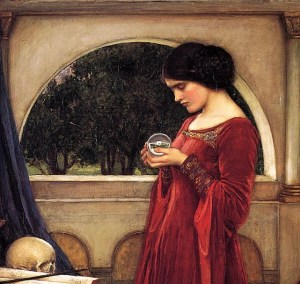
\includegraphics[scale=.5]{a20121210KnowledgeoftheFuture-img001.jpg} 
\end{wrapfigure}

This knowledge of the future baffles the rational mind, since it claims that the future can be known only if it be predetermined. However, this is a misunderstanding of what it means “to know”, since it places knowability in the object of knowledge rather than in the knower himself. Hence we are compelled to not consider the thing known, but rather we need to grasp how the knower knows. Following Augustine and the Neo-Platonists (and anticipating Rene Guenon, to be sure), Boethius first distinguishes between eternity and everlastingness. The latter is perpetual existence in time, whereas the former is outside time altogether. Boethius explains:

\begin{quotex}
The world is still not such that it may properly be considered eternal … Its life may be infinitely long, but it does not embrace and comprehend its whole extent simultaneously. It still lacks the future, while already having lost the past. So that that which embraces and possesses simultaneously the whole fullness of everlasting life, which lacks nothing of the future and has lost nothing of the past, that is what my properly be said to be eternal. … It is one thing to progress through everlasting life, and another thing to have embraced the whole of everlasting life in one simultaneous present. This is clearly a property of the mind of God. 

\end{quotex}
Boethius follows Plato's claim that “God is eternal, the world perpetual.” For the world, the past is always receding (“lost”) while the future is not yet (“lacking”). Thus God cannot be considered as existing “before” the world. Hence, it is not really a question of foreknowledge of the future, but instead the “knowledge of a never ending presence.” This is the literal meaning of Providence, “looking forth”, which he contrasts to prevision or “seeing ahead”.

Next, Boethius addresses the counterargument that to know future events implies that the future is determined and free will is not possible. Obviously, this is mechanical thinking arising from the rational mind as opposed to the organic thinking that sees time as a whole. If I watch you walking down the street, then I know it through sense perception; nevertheless, this type of knowing, which is also a form of direct intuition, does not make your perambulation unfree or necessary.

By analogy, and that is all we may have for now, the same can be said about God's seeing through intellectual intuition. Boethius writes:

\begin{quotex}
Divine foreknowledge does not change the nature and property of things; it simply sees things present to it exactly as they will happen at some time as future events. … the divine gaze looks down on all things without disturbing their nature; to Him, they are present things, but under the conditions of time they are future things. And so when God knows that something is going to occur and knows that no necessity to be is imposed on it, it is not opinion, but rather knowledge founded upon truth. 

\end{quotex}
In the example of watching someone walk on the street, we were clearly appealing to spatial perception rather than temporal. It is easy to grasp that our experience of objects in space is grasping the whole, as something all-at-once, at least within the limits of our horizon. But events in time don't typically have that same effect, as events come at us sequentially, not all at once. Each moment in time seems independent of what follows; this is what perplexed Hume so that he could not understand the nature of causality. Yet as we recently pointed out\footnote{\url{https://www.gornahoor.net/?p=5381}}, artistic inspiration often takes this form. This is why Solovyov used artistic experience as the model for the type of intuition being described. In particular music and poetry lend themselves to this, this they unfold in time while being grasped as a whole. Hence, we can grasp a symphony as a whole even though our experience is one note after another. Yet, the musicians play the instruments by their own free will.

It may be helpful to draw on what \textbf{Rene Guenon} writes about time in The Reign of Quantity. He points out that time is more subtle than space, and that accounts for its elusiveness. It can only be measured by spatial criteria and the most intimate part of us — our mental life — develops in time yet has no spatial character. This means that time is even more qualitative than space and our tendency to experience time just in its quantitative aspect can only result in misunderstanding. Guenon uses the example of the four seasons, the temporal equivalent of the four spatial directions. Once we see things in terms of cycles — organically — we can “predict” the future. Of course, the world unfolds in cycles within cycles, etc.

Next, we can point out the nature of manifestation. Recall that a fundamental principle is the identity of knowing and being. We know that there are possibilities of manifestation. When God knows a possibility of manifestation, as he must since it is an idea in His own mind, then it necessarily manifests—essence and existence are one. And this is so, even if from the perspective of time, it is the result of free acts.

Finally, how can man experience things \emph{sub specie aeternitatis}? Obviously, not man qua man, but only from states that are higher than the human state. To reach that highest state is what Guenon calls deliverance as opposed to salvation. Readers who continue to do their exercises and meditations may find that they can reach a state of detachment in which consciousness is observing the actions of the body. Within the incessant states of conscious activity, that is, the everlasting or perpetual, what is the one constant? That is the eternal.



\flrightit{Posted on 2012-12-10 by Cologero }

\begin{center}* * *\end{center}

\begin{footnotesize}\begin{sffamily}



\texttt{Saladin on 2013-10-18 at 13:25 said: }

Very interesting! I have just discovered The Consolation of Philosophy, and it is a real gem!


\end{sffamily}\end{footnotesize}

\section{Gods, Angels, and Men}

Every now and then, it is necessary to go over some basic concepts, particularly because the way we use them is not necessarily how they are commonly used. The claim of metaphysics is that it leads to perfect gnosis. As such, it is not a theory, a set of beliefs, or mere opinion; rather, it sees things as necessarily true. Moreover, besides the formal knowledge of the ideas, principles, and concepts, a change in being is also necessary to turn that knowledge into gnosis. One “sees” that it is so; at some point, as that gnosis sinks in, it becomes impossible to see the world in any other way.

Few men concern themselves with issues of epistemology; that is, they seldom concern themselves with the reasons for their beliefs. A thought crosses their mind, they are pleased with it, probably it brings them esteem in their social circle, it provides a modicum of order to the unstoppable stream of consciousness, and it is imprinted with a strong emotional attachment. Hence, it must be true and they defend that opinion fervently. We metaphysicians, on the other hand, are not so sanguine. We realize how difficult it is to achieve even the beginnings of knowledge. We endure the hardships of the spiritual combat, clearing out mind of the debris of unsupportable opinions. The Muslim sage, \textbf{Suhrawardi}, says there are four categories of men who seek after knowledge. The task at hand is to move from (1) to (4).

\begin{enumerate}
\item Those who feel the thirst for knowledge and embark upon the path of seeking it. 
\item Those who have attained formal, or discursive, knowledge, but not yet gnosis. 
\item Those who have achieved gnosis or intellectual intuition, but not discursive knowledge. Many saints fall into this category, since they may not necessarily have the proper metaphysical instruction 
\item Those who have perfected discursive knowledge as well as gnosis and intellectual intuition. 
\end{enumerate}
\paragraph{Being and God}
This issue comes up often, so this would be a good time to go over it again. Guenon makes the claim that the primordial unity is universal being. As Being is the principle of any existing thing, this is understood as God in the Western classical tradition. Since it is a unity, it must be monotheism. This is precisely what is meant, and we reject any anthropomorphic god, or even a “personal” god. Unfortunately, to those ignorant of metaphysics, they presume these false and idolatrous notions of God.

To deny this principle, therefore, is to reject the unity of being. One alternative would be complete chaos, or an indeterminate universe like some enormous Schroedinger cat. That would be like the matrix, with the mind confabulating a coherent worldview out of the random universe, not unlike the mind during sleep fabricating dreams out of random neural impulses.

Or else, there are two or more irreconcilable principles with no unifying higher principle. An example is Manichaeism, with an infinite and pointless battle between good and evil. In ancient paganism, the gods and goddesses were independent, some giving their blessings to a project and others, curses. They themselves are not ultimate, but are subject to the Fates.

Now this understanding of God is common to all Tradition. For example, in the Aristotelian-Thomist tradition mentioned in the Round Table, God is understood as Being. The Muslim metaphysician, Avicenna, says substantially the same thing. God is the necessary Being, the only such Being, and all other beings are contingent. Now these days, you can easily run across web sites that try to demonstrate that Christians and Muslims do not “believe” in the same God. To the contrary, as was just shown, the understanding of God is basically the same, and could not be otherwise. The real question is whether Traditional Christianity is compatible with Protestantism. Even more so, is Mormonism incompatible with this view; they really believe in some sort of demiurge that they name god. Esoterically, one's allies are other than what seems obvious exoterically.

\paragraph{Angelic Intelligences}
As the gnosis of God was lost in the West and He became regarded as just another being or person, albeit of great powers, so too did knowledge of the angels. In large part this was due to the hyper-rationalism that discredited \textbf{Dionysius the Areopagite} and \textbf{Hermes Trismegistus} because of the allegedly later dates attributed to their writings; this was also related to the false doctrine of Sola Scriptura. The Hermetic tradition did keep it alive, and we see that also in \textbf{Valentin Tomberg}. Tomberg pointed to Rudolf Steiner primarily for his writings on spiritual hierarchies, but we will see what it would mean to restore knowledge of this realm.

The Muslim tradition, or at least one branch of it, did however keep this knowledge alive. They regarded Pythagoras, Hermes, and Plato, among others, as the bearers of an ancient, but still valid, tradition. \textbf{Avicenna}, for example, has a cosmology not unlike the one we indicated in Spiritual Beings\footnote{\url{https://www.gornahoor.net/?p=1941}}. For him, the process of creation is the same as intellection. Keep in mind that angels are pure intellects, hence, non-formal beings. As each level in the angelic hierarchy contemplates the ideas, the world is created until the physical world, which is the final stage in the actualization of possibilities.

Our experience of the ideas is obviously not through the senses, but rather as thoughts. Thus, when we observe the thoughts that appear in consciousness, we are contemplating along with the angels. We recognize how ideas in the fullness appear as constellations of related thoughts. The more detached we are, the higher we can rise to experience more and more subtle realms. Unfortunately, the way is usually blocked by the “spirits of the air”, that is, demonic intelligences that fill our minds with counter-creative ideas. This is why “watchfulness” is so necessary to achieve gnosis, so we can “see” the source of all those thought forms that influence and control our actions.

At a still lower level, the erotic and thymotic impulses work in consciousness. They each have an intellectual component, and thoughts related to these impulses form a very large part of our daily consciousness. Spiritual training is therefore focused on the observation of thoughts.

\paragraph{Man and Free Will}
\begin{quotex}
Omnipotence does not mean power to do absurdities. The compulsion of another's will is such an absurdity, and therefore no real omnipotence could force such a compulsion. Omnipotence is spiritual, and spirit acts not by brute compulsion but by knowledge and inspiration. \flright{\textsc{R. G. Collingwood}}

\end{quotex}
Man, as spirit, has free will. Higher intelligences, therefore, cannot “take over” a mind; however, a mind can latch onto a thought, harbor it, and freely make it a part of his own identity. Often after a tragic event, people will plaintively ask, “Why did God allow this to happen?” However, to forcibly prevent a free man from acting, is an absurdity, such as making a square triangle. He simply would not be what he is. The real task, then, is to increase knowledge and to be inspired by the higher intelligences.

Yet men are not equal in their intelligences. A hierarchical society will provide the visual guidance to those unable, or not yet able. For example, the Brahmin type is idealist and objective, while the Kshatriya is idealist and subjective. The former contemplates things objectively; the latter is oriented to action. Hence, his subjectivity is crucial when administering a state or conducting a war, since he needs to take sides. The vaisya is objective but materialist; hence he can work in science and industry, the business of the world. The shudra is subjective and materialist, hence, incapable of true self-government.

In an organic society, the various castes work in harmony until, through degeneration the lower castes will rebel against the higher. At our time, the highest caste is disorganized, and the levers of power are in the hands of the shudra. On their own, they cannot have a direct conception of God and higher intelligences, which is why societies ruled by shudra tend to be atheistic and oriented to the satisfaction of material desires, including base and perverse desires.

These are the clues to understand events from a transcendent perspective. The first task is to understand man and his types, caste being fundamental. When the characteristics of each caste are understood, events and the reasons for decisions and actions will become clear. Beyond that, one learns to see intuitively the various higher forces that strive to influence the world; these are generally of three types: constructive, preservative, or destructive. One will see how various thought forms take hold in men; it is still amazing how groups of men will suddenly latch onto a new idea at the same time. Their makeup predisposes them to accept it.


\hfill

References:

Nasr, Seyyed Hossein, Three Muslim Sages

Schuon, Frithjof, Castes and Races



\flrightit{Posted on 2013-06-25 by Cologero }

\ \begin{center}* * *\end{center}

\begin{footnotesize}\begin{sffamily}



\texttt{Ash on 2013-06-26 at 01:53 said: }

The relationship between knowledge and gnosis is interesting. The third type described here would likely be difficult for many of us to encounter precisely because we could not waste time on sophistry and intellectual pride on them. The holy fool is the most clear example – good luck trying to talk about “the essence of Being”, political ideologies, or Heidegger with them. While we try to think our way to Heaven, Heaven finds itself on earth in them and shakes its head in bewilderment.

The idea of the angelic intelligences is one I will have to ponder further. It seems to be a short step from “acting” spiritual entities to the “acting” God to the anthropomorphic God. Father Seraphim Rose's doctrine of the toll houses troubles some of his followers in a similar way…it seems to be too corporeal at least at first glance. I find it interesting that the personalization of God was referred to as idolatry. This leads to a topic I often wonder about: how exactly aspects of exoteric relation are brought into an esoterically minded person's life. Tradition, of course; but how do we approach the Bible, with its very personal God and tribal histories? Christ the Logos, yes; but what of Jesus the Teacher and Carpenter? As a Catholic, Cologero, I'm sure you have encountered this as well in some form. 

The way the demonic intelligences are discussed here remind me very much of how they are presented in Lewis' The Screwtape Letters, a book a highly recommend. Not a word wasted.

“When two humans have lived together for many years it usually happens that each has tones of voice and expressions of face which are almost unendurably irritating to the other. Work on that. Bring fully into the consciousness of your patient that particular lift of his mother's eyebrows which he learned to dislike in the nursery, and let him think how much he dislikes it. Let him assume that she knows how annoying it is and does it to annoy – if you know your job he will not notice the immense improbability of the assumption. And, of course, never let him suspect that he has tones and looks which similarly annoy her. As he cannot see or hear himself, this easily managed.” 

“Indeed the safest road to Hell is the gradual one–the gentle slope, soft underfoot, without sudden turnings, without milestones, without signposts,…Your affectionate uncle, Screwtape.”


\hfill

\texttt{Jacob on 2013-06-26 at 11:47 said: }

I have some trouble with the personal God concept as well. Hopefully, Cologero can help clarify for me. I know Charles Upton once pointed out that when we say something is non personal we equate it with a non intelligent force like Gravity. So he used the word Transpersonal, something transcend to personhood. That helps point towards an answer, but it's still very difficult for me to grasp, especially with the problems you point out, Ash. 

@Cologero and Logres: BM's Gnosis I should arrive today. I'm looking forward to reading it. I'll probably have to return with questions though.


\hfill

\texttt{Avery on 2013-06-26 at 12:29 said: }

At least in my mind's eye, the existence of angels makes perfect sense to me. Devils clearly exist (I agree that The Screwtape Letters, one of the best books of the 20th century, comes in handy here, and Evola makes a compelling but somewhat less poetic case in Ruins as well); devils are intermediaries, and it is odd to suggest the evil one can make intermediaries but God cannot; therefore angels should exist too.

G.K. Chesterton wrote, “The human race, according to religion, fell once, and in falling gained the knowledge of good and of evil. Now we have fallen a second time, and only the knowledge of evil remains to us.” It would be irresponsible to rely on one's sense of evil without enriching the much more important sense of good.


\hfill

\texttt{Avery on 2013-06-26 at 12:29 said: }

At least in my mind's eye, the existence of angels makes perfect sense to me. Devils clearly exist (I agree that The Screwtape Letters, one of the best books of the 20th century, comes in handy here, and Evola makes a compelling but somewhat less poetic case in Ruins as well); devils are intermediaries, and it is odd to suggest the evil one can make intermediaries but God cannot; therefore angels should exist too.

G.K. Chesterton wrote, “The human race, according to religion, fell once, and in falling gained the knowledge of good and of evil. Now we have fallen a second time, and only the knowledge of evil remains to us.” It would be irresponsible to rely on one's sense of evil without enriching the much more important sense of good.


\hfill

\texttt{Matt on 2013-06-26 at 17:28 said: }

Jacob,

I think what Cologero is getting at with the idea of God not being a person is a fundamental distinction between the classical theist tradition – part of Tradition itself – and what is known as “theistic personalism” which is advocated by thinkers like William Lane Craig, Plantiga, and Swinburne. Theistic personalism is also what most protestants believe and probably even what the average Catholic in the laity believes in – sadly.

The classical theist tradition affirms that while God is person-like, that does not mean God is tantamount to being a person jut like us, except with qualities to the maximal degree. Its the opposite with theistic personalists – when they say God is a person, they believe that God is a person just like us. It gets down to how they view the divine attributes. Classical theism views the divine attributes in an analogous way – there is something of the reality of God that is analogous to the will and intellect within us – whereas theistic personalists view God's attributes in a univocal way, so his personal attribute is just like our personhood, but to the maximal degree like all of His other attributes such as power (same as as ours but to the “max”), and goodnes (he is a moral agent that is maximally good instead of the Sovereign Good). The A-T philosopher Edward Feser, whom Cologero has mentioned a few times here, goes into detail about this fundamental difference and why theisitc personalism is so problematic. He makes the apt comparison of the theisitc personalists' god to how much of the historical greek religion viewed Zeus – just a being among a class of beings, though a very exceptional one (instead of the Being of beings, Being Itself). Feser also makes the similar comparison to Superman, which I think is also an appropriate one.


\hfill

\texttt{Jacob on 2013-06-26 at 19:38 said: }

Ok, thanks Matt. That helps a lot. Also explains why the Kalam argument theistic philosophers use so often grew out of a discipline most Muslims scholars looked down upon.


\hfill

\texttt{Matt on 2013-06-26 at 19:59 said: }

No problem Jacob.

How theistic personalists view God's attributes is the main reason why they don't accept divine simplicity, the convertibility of the transcendentals – the Oneness of God essentially. Since our attributes are metaphysically separate, and if God's attributes are just like ours, then God's attributes are therefore also metaphysically separate. They also think that God – classically/traditionally conceived – can not have accidental properties, but it doesn't seem like they've taken into consideration that God classically concieved can have what is called `Cambridge properties”. 

This has a number of logical implications – most of which I don't think have been considered by theistic personalists – in relation to the fundamental tenets of Christianity (and probably Tradition as a whole). If God really is indeed composed of parts, then one can't really say God is infinite (The Infinite is a better term) since God would now have intrinsic boundaries. And, at least to me, I don't see how the fundamental Christian tenet of the Logos as the common principle that unities all is compatible with theistic personalism.


\end{sffamily}\end{footnotesize}


\chapter{Notes on metaphysics}
\section{Oriental Metaphysics}

\begin{quotex}
The greatest of all lessons is to know one's self. For if one knows himself, he will know God; and knowing God, he will be made like God, not by wearing gold or long robes, but by well-doing, and by requiring as few things as possible.\footnote{\url{https://www.newadvent.org/fathers/02093.htm}} \flright{\textsc{Clement of Alexandria}, \emph{The Paedagogus}}

The soul is all that it knows. \flright{\textsc{Aristotle}, \emph{On the Soul}}

The conceptions of Aristotle are in complete agreement with those of the East. \flright{\textsc{Rene Guenon}, \emph{Man and his Becoming}}

Dear Unknown Friend, do not scorn mediaeval scholasticism. It is, in truth, as beautiful, as venerable and as inspiring as the great cathedrals that we have inherited from the Middle Ages. To it we owe a number of masterpieces of thought—thought in the light of faith. And, like all true masterpieces, those of mediaeval scholasticism are beneficial. They heal the disorientated, feverous and confused soul. What is at stake with scholasticism is God, the soul, freedom, immortality, salvation, good and evil. Therefore, do not despise mediaeval scholasticism, dear Unknown Friend; it is still of value. \flright{\textsc{Valentin Tomberg}, \emph{Meditations on the Tarot} }

\end{quotex}
In a letter to Guido De Giorgio\footnote{\url{https://www.gornahoor.net/?p=4460}}, Rene Guenon mentioned that he had given a lecture to a study group at the Sorbonne in 1925\footnote{The text of that lecture can be found at Oriental Metaphysics: \url{https://www.gornahoor.net/library/OrientalMetaphysics.pdf .}}. This post is a summary of that lecture. In it, most of Guenon's main themes are covered. The text seems straight forward after a cursory reading, yet many people seem to struggle with the ideas. On the one hand, this may lead to confusion where there is none, and on the other, to widely speculative notions that have no basis in fact, and are, mere diversions.

Keep in mind that Guenon is not an original thinker, and, in his case, that would be a compliment. However, he has provided a valuable task of synthesis, and more importantly, he has demonstrated how metaphysical knowledge, which used to be known, has all but disappeared in the West. That does not mean, however, what many seem to think it means. The teachings are available in plain sight; what is missing, apparently, is how to transform rational knowledge into spiritual realization.

\paragraph{Metaphysics}
In itself, metaphysics is neither Eastern nor Western. Guenon deals with “Oriental” metaphysics because in the West such knowledge

\begin{quotex}
is a thing forgotten, generally ignored, and almost entirely lost, while in the East it still remains the object of effective knowledge. 

\end{quotex}
Guenon mentions specifically Hinduism, Taoism, and Islam where the true metaphysics can be found. In 1925, Guenon concedes that he was most familiar with Hindu metaphysics.

He is more sanguine about the East in 1925 than I am in 2020. China has been irreligious for four generations, and I have yet to meet a Chinese national familiar with Taoism. I don't know about the state of Islamic metaphysics; there are two mosques in town, but they don't advertise esoteric schools to the general public. At that time, Guenon did not consider Buddhism to be a valid tradition, although today it is more missionary than either Taoist or Islamic esoterism. Hinduism, on the other hand, is widely available in the West in the intervening years since Guenon's lecture.

I used to give talks and lead classes at a metaphysical bookstore in Deerfield Beach. There I met many Western students of Hindu doctrine, even gurus from India and their America acolytes. When I was leading a weekly class on Guenon, none of the Western Hindus recognized anything corresponding to their understanding. Usually, they were more interested in reincarnation, and even adopting Indian styles of dress and cuisine. Indian tech workers in the USA are typically more interested in technical subjects and practice their exoteric rites. I asked a group how many had read the Bhagavad Gita; the response was none. Guenon claims that is normative in Hinduism, since individuals absorb as much of the esoteric doctrine that suits their abilities.

So I decided to focus on the recovery of the Western Tradition. This decision is justified because Taoism and Islam are restricted, and there are too many fraudulent Hindu gurus in the West:

\begin{quotex}
these doctrines are reserved for a relatively restricted and closed elite [in Taoism and Islam]. This was also the case in the West in the Middle Ages, in an esotericism comparable in many respects to that of Islam and as purely metaphysical as the Islamic one; of this the moderns, for the most part, do not even suspect the existence. 

\end{quotex}
\paragraph{Western Metaphysics}
The notion of a common metaphysics across traditions was not unknown in the West, for example Medieval Scholasticism drew on:

\begin{itemize}
\item Pagan metaphysics, particularly Aristotle and Plato 
\item Influence of Arabic and Islamic Philosophy on the Latin West\footnote{\url{https://plato.stanford.edu/entries/arabic-islamic-influence/}}, including al-Fārābī, Avicenna, and Averroes 
\item Hebrew metaphysics, at least via Maimonides 
\end{itemize}
Had they known about it, they probably would have included Hindu metaphysics. So Guenon is preaching to the choir here.

\paragraph{Intuition}
Reason is a human feature and thus is fully natural. If physics is the study or the natural world, then metaphysics is the study of the supernatural, i.e., what is beyond the human state. The method of knowing the supernatural is “intuition”, that is, a direct understanding of metaphysical ideas. It is analogous to sensory intuition, but differs since it does not involve the senses. Intuition is beyond Reason, so that bookish knowledge is not at all what Guenon means. Nevertheless, such knowledge use usually necessary as preparation.

\paragraph{Realization}
Therefore, metaphysical doctrines must be “realized”, not just “known”. Specifically, they must be made “real” and to do so requires the transcendence of the merely human state. The indispensable means to such realization is \textbf{Concentration}. Guenon explains:

\begin{quotex}
There is nothing in common between metaphysical realization and the means leading to it, or, if preferred, which prepare for it. This is why, moreover, no means are strictly or absolutely necessary; or at least there is only one indispensable preparation, and that is theoretical knowledge. This, on the other hand, cannot go far without a means which will play the most important and constant part: This means is \emph{concentration}. 

\end{quotex}
Many readers get hung up at this point. Instead of learning concentration, they believe that they just need to read yet another book to explain it. However, what they really need is to learn concentration, which is the very first thing an esoteric school will teach you. Unfortunately, there is no “method” or “recipe” for this, since the means “have to be adapted to the temperament of each individual and to his particular aptitudes and disposition.” Perhaps it will be helpful to describe some particular exercises.

\textbf{Soul Awareness}. Aristotle and the Scholastics taught that plants, animals, and humans each add to the layers of the soul. These correspond to the sheaths or koshas of the Vedanta\footnote{\url{https://www.gornahoor.net/?p=9647}}. One can learn about them simply as a doctrine, using the faculty of Reason, or one can realize it through intellectual intuition.

To do that, one needs to learn to concentrate on the observation of one's inner states: i.e., all the sensations, emotions, fantasies, thoughts, etc. Through these observations, he will see directly the operations and interactions of the vegetative, sensitive, and intellectual souls. Obviously, that is a huge task and will take some time. We can't provide a guidebook here, but ultimately one wants to be able to become the master of one's inner states.

\textbf{The Unmoved Mover}. Guenon refers to Aristotle's notion of the unmoved mover several times in his writings. Specifically, this means the principle of manifestation, which is motion and action, must be actionless. As a concentration exercise, sit still and silently and passively observe whatever appears in consciousness. You should observe random changes. In the midst of them, try to find the “unmoved mover”, that is, what does not change while everything else is changing.

\paragraph{Primordial State}
This realization of the integral individuality is described by all traditions as the restoration of what is called the “primordial state” which is regarded as man's true estate and which moreover escapes some of the limitations characteristic of the ordinary state, notably that of the temporal condition. The person who attains this “primordial state” is still only a human individual and is without effective possession of any supra-individual states; he is nevertheless freed from time and the apparent succession of things is transformed for him into simultaneity; he consciously possesses a faculty which is unknown to the ordinary man and which one might call the “sense of eternity.”

This is of extreme importance, for he who is unable to leave the viewpoint of temporal succession and see everything in simultaneity is incapable of the least conception of the metaphysical order.

\begin{quotex}
Why this appellation of “primordial state”? It is because all traditions, including that of the West (for the Bible says nothing different) are in agreement in teaching that this state was originally normal for humanity, whereas the present state is merely the result of a fall, the effect of a progressive materialization which has occurred in the course of the ages, and throughout the duration of a particular cycle. 

\end{quotex}
There is not much to add to this except for this point. In a lecture by a hand-picked student of a guru, she mentioned the Fall, but also said she did not know the reason for it. On the other hand, the dominant Western Tradition of the past two millennia does provide a deeper understanding, which can even be verified through its effects on consciousness.

\paragraph{Higher States}
The Primordial State is still a human state, so Guenon describes higher states, as summarized:

\begin{itemize}
\item \textbf{Ordinary Human state} = result of a fall 
\item \textbf{Primordial state} = realization of the integral individuality. Freed from time. Sense of eternity. Originally normative for the human 
\item \textbf{Supra-individual but still conditioned}. Includes substates in these categories: 

\begin{itemize}
\item Informal but still pertaining to manifested existence 
\item Universality which is pure being 
\end{itemize}
\item Principle of all manifestation or Deliverance. “In this unconditioned state all other states of being find their place, but they are transformed and released from the special conditions which determined them as particular states.” 
\end{itemize}
Deliverance means being in possession of the fullness of one's own potentialities. It is the state of absolute plenitude. Limiting conditions, or privations, disappear. The human state is a mix of Act and Potency, or Essence and Existence. As the potential becomes actualised, one gets closer to God, for Whom there is not privation so Essence and Existence coincide.

\paragraph{Phenomena}
These states have nothing to do with woo-woo. That is, these states have nothing to do with preternatural phenomena, visions, healing, powers, out of body experiences, channeling, or other unusual happenings. These are still part of the physical, not metaphysical, order. Such phenomena do not in themselves indicate the states of metaphysical realisation, even should they appear as side-effects.

\paragraph{Source of Teachings}
Tradition has no human origin in time. It was known in the Primordial State but forgotten in the Fall. The Tradition has taken various exterior forms. Augustine recognized this in his claim that there is just one Religion, which is now called the Catholic religion, at least in the West.

Metaphysical knowledge, as well as the realization that will turn it into all that it truly ought to be, is thus possible everywhere and always. This means that initiation by an esoteric group is not strictly speaking necessary. We have already shown that it is not even sufficient.

Metaphysical realization cannot be achieved by human means alone. Rather, it is a gift and one can only prepare to receive and recognize it.



\flrightit{Posted on 2020-07-12 by Cologero }

\begin{center}* * *\end{center}

\begin{footnotesize}\begin{sffamily}



\texttt{Adil on 2020-07-18 at 17:48 said: }

“The Tradition has taken various exterior forms. Augustine recognized this in his claim that there is just one Religion, which is now called the Catholic religion.”

This makes me think of the recent conversion of the Agia Sophia back into a mosque. The West (including Eastern Orthodox churches) have not been late to condemn this move. But in reality, what has changed? Agia Sophia was a mosque for 500 years, until it was turned into a secular museum. Inside it, you can see a blend of Islamic and Christian art. Now, it has once again been turned into a sacred space, instead of a poorly maintained museum piece with an entrance fee.

Don't get me wrong. Ideally, the cathedral would be used as a church, but history is what it is. This wasn't exactly unexpected. At least, somone will now feel responsible for the building, and perhaps not let it fall apart. If the west was serious with its critique, perhaps it could respond by forbidding any mosques in Europe, and turn the existing ones into museums?


\end{sffamily}\end{footnotesize}

\section{Notes to Oriental Metaphysics}

I've been cleaning up paperwork. I stumbled across some personal musings that go back decades. The topics then are similar to those of today, although the approach was quite different. I also found some class notes for a discussion group on Oriental Metaphysics by Rene Guenon. They date back to November 2005. The audience was primarily Theosophists and Vedantists, who had little understanding of metaphysics. The following notes were geared to them. They are merely an introduction to certain concepts. I have only found the notes for the first class. In retrospect, further notes were probably not necessary as we went straight to the text.

\begin{quotex}
The consummation of the infinite End, therefore, consists merely in removing the illusion which make it seem yet unaccomplished. The good, the absolutely Good, is eternally accomplishing itself in the world: and the result is that it needs not wait upon us, but is already by implication, as well as in full actuality, accomplished. This is the illusion under which we live. It alone supplies at the same time the actualizing force on which the interest in the world reposes. In the course of its process the idea creates that illusion, by setting an antithesis to confront it; and its action consists in getting rid of the illusion which it has created. Only out of this error does the truth arise. In this fact lies the reconciliation with error and with finitude. Error or other-bine, when superseded, is sill a necessary dynamic element of truth; for truth can only be where it makes itself its own result.

\flright{\textsc{Hegel}, \emph{Logic}}

The dominant note of barbarism is will and that of culture, especially the culture influenced by Greek ideas, is reason or intellect, so that of Christendom is love.

\flright{\textsc{Martin D'Arcy}, \emph{The Mind and Heart of Love}}

\end{quotex}
\paragraph{Aporia}
Aporia is an insoluble contradiction or paradox in a text's meanings. (The end result of dialog.)

\paragraph{Stages of Rationality}
\begin{wrapfigure}{rt}{0.35\textwidth}
 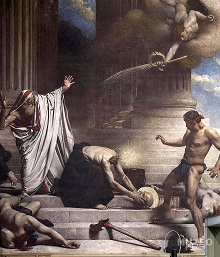
\includegraphics[scale=.7]{a20201222NotestoOrientalMetaphysics-img001.jpg} 
\caption{Losing one's head, finding ones' heart}
\end{wrapfigure}

\begin{itemize}
\item \textbf{Subrational.} The subrational is characterized by instinct, impulse, elan vital, unchecked will. Lacking an inner check or desires, subrational societies rely on custom and taboo to control behaviour. These often seem quite irrational to outsiders. 
\item \textbf{Rational.} Reason gives man much power of nature, and to a lesser extend, over his own passions. However, every assertion creates its opposite, every Yes a No, every Idea its antithesis. These antinomies result in interminable — and irresolvable — discussions. “Reasonable men can agree to disagree”, which demonstrates, not the value of reason, but its impotence to lead to any kind of genuine knowledge. 
\item \textbf{Surparational.} The suprational, or metaphysical intuition, is above reason, yet not irrational. Dualities are resolved, and there is a genuine knowledge (gnosis). Identifying characteristics are: 

\begin{enumerate}
\item Conforms to experience 
\item Coherent 
\item Consistent with natural knowledge 
\end{enumerate}
\end{itemize}
\paragraph{Occam's Razor}
\emph{One should not increase, beyond what is necessary, the number of entities required to explain anything.}

It is necessary to resist the temptation to postulate entities such as “higher” and “lower” minds, etc. The fundamental insight is to realize the unchanging and eternal that subtends every experience. This is the Witness, or Self, which is \emph{not} a postulated entity, since it can never be an “object” to anything.

Reading a work like Oriental Metaphysics is in invitation to achieve such self-realization.

\paragraph{Degrees of Experience}
Here are some distinctions to keep in mind:

\begin{itemize}
\item \textbf{Metaphysical Intuition}. This is the realization of the Atman, Self, Witness. It is beyond any particular state of being, and beyond any particular experience. It is beyond nature. 
\item \textbf{Mystical Experience}. This is an experience of a state of being higher than the human state. Although such experiences may be rapturous, ecstatic, extraordinary, insightful, and peaceful, they still belong to the phenomenal realm. This is what distinguishes such an experience from metaphysical intuition. 
\item \textbf{Paranormal Experience}. This is an experience of the subtle (i.e., non-physical) realms of the human state. 
\item \textbf{Demonic Experience}. “Demons” are particular constellations of thought patterns that can influence behavior. Since the ego often identifies with such patterns, it considers them its own, and is in bondage to them. As such, this is akin to “demonic possession”. 
\end{itemize}
Guenon is careful to strongly distinguish Metaphysical Intuition from particular experiences. Mystical and paranormal experiences are still in the psychic or psychological realm.

\paragraph{Characteristic Signs}
\begin{itemize}
\item \textbf{Ataraxy}. Tranquility, imperturbability. State of soul which is peaceful, undisturbed by events, either external, or even internal, such as thoughts, fantasies, desires, emotions. 
\item \textbf{Apatheia}. This is not the Stoic state of freedom from emotions, but rather freedom from “passions”, rightly understood. They are negative emotions contrary to nature (not nature just limited to the physical!). Examples: conceit, gluttony, lust, vanity, greed, malice. Some emotions may or may not be contrary to nature, depending on their object: anger, hatred, sorrow, fear.

Similarly, some legitimate pleasures and desires are not necessarily passions. One obvious example is the feeling of Bliss (Ananda) which accompanies metaphysical realization. 
\item \textbf{Agape}. More than friendship, family affection, or erotic attraction. This is spiritual love. 
\end{itemize}
\paragraph{Lessons to be Learned}
It has been said that life is a school, where lessons are to be learned. If so, it is a strange sort of school where we are not only not given the answers to the question, we are not even given the questions. If lessons are to be learned, we seldom see it. Instead there are the same mistakes repeated, plans gone awry, potentials unfulfilled, resolutions broken, love unrequited.

Desire is insatiable, no sooner is one fulfilled, than a dozen others arise to take its place. If there is a lesson to learned, it must be this:

There is no solution within life.

Isn't this also Buddha's conclusion, or Jesus' assertion that “My kingdom is not of this world”? The solution is in another direction, unnatural, or better, supernatural (in the true meaning of this term). Therein lies deliverance.

Only the human state offers the possibility for deliverance (or Beatific Vision).

\paragraph{One Thing Needful}
With it, there is not doubt; without it, there is no understanding.

This is the realization of the Self that witnesses, but is not witnessed.

Prakriti (matter) brings into manifestation (multiplicity) Purusha (spirit).

What does the Witness witness when it is witnessing?



\flrightit{Posted on 2020-12-22 by Cologero }


\end{document}
